\documentclass[]{article}
\usepackage{lmodern}
\usepackage{amssymb,amsmath}
\usepackage{ifxetex,ifluatex}
\usepackage{fixltx2e} % provides \textsubscript
\ifnum 0\ifxetex 1\fi\ifluatex 1\fi=0 % if pdftex
  \usepackage[T1]{fontenc}
  \usepackage[utf8]{inputenc}
\else % if luatex or xelatex
  \ifxetex
    \usepackage{mathspec}
    \usepackage{xltxtra,xunicode}
  \else
    \usepackage{fontspec}
  \fi
  \defaultfontfeatures{Mapping=tex-text,Scale=MatchLowercase}
  \newcommand{\euro}{€}
\fi
% use upquote if available, for straight quotes in verbatim environments
\IfFileExists{upquote.sty}{\usepackage{upquote}}{}
% use microtype if available
\IfFileExists{microtype.sty}{%
\usepackage{microtype}
\UseMicrotypeSet[protrusion]{basicmath} % disable protrusion for tt fonts
}{}
\usepackage[margin=1in]{geometry}
\ifxetex
  \usepackage[setpagesize=false, % page size defined by xetex
              unicode=false, % unicode breaks when used with xetex
              xetex]{hyperref}
\else
  \usepackage[unicode=true]{hyperref}
\fi
\hypersetup{breaklinks=true,
            bookmarks=true,
            pdfauthor={Benjamin Weigel},
            pdftitle={WEB350},
            colorlinks=true,
            citecolor=blue,
            urlcolor=blue,
            linkcolor=magenta,
            pdfborder={0 0 0}}
\urlstyle{same}  % don't use monospace font for urls
\setlength{\parindent}{0pt}
\setlength{\parskip}{6pt plus 2pt minus 1pt}
\setlength{\emergencystretch}{3em}  % prevent overfull lines
\setcounter{secnumdepth}{0}

%%% Use protect on footnotes to avoid problems with footnotes in titles
\let\rmarkdownfootnote\footnote%
\def\footnote{\protect\rmarkdownfootnote}

%%% Change title format to be more compact
\usepackage{titling}

% Create subtitle command for use in maketitle
\newcommand{\subtitle}[1]{
  \posttitle{
    \begin{center}\large#1\end{center}
    }
}

\setlength{\droptitle}{-2em}
  \title{WEB350}
  \pretitle{\vspace{\droptitle}\centering\huge}
  \posttitle{\par}
  \author{Benjamin Weigel}
  \preauthor{\centering\large\emph}
  \postauthor{\par}
  \predate{\centering\large\emph}
  \postdate{\par}
  \date{10/01/2015}

\usepackage{booktabs}
\usepackage{graphicx}
\usepackage{longtable}
\usepackage{tocloft}
\usepackage{rotating}


\begin{document}

\maketitle


\tableofcontents\clearpage

\begin{table}[ht]
\centering
\begin{tabular}{rlllrr}
  \toprule
 & substance & fragment & formula & MW & mz \\ 
  \midrule
1 & naringenin & 1,4B+-2H &  &  & 147.04 \\ 
  2 & naringenin & 1,4B+-2H-2CO &  &  & 91.05 \\ 
  3 & naringenin & 1,4B+-2H-CO &  &  & 119.05 \\ 
  4 & naringenin & AC+ &  &  & 179.03 \\ 
  5 & naringenin & [M+H]+ & C15H12O5 & 272.07 & 273.08 \\ 
  6 & naringenin & [M+H-2C2H2O]+ & C15H12O5 & 272.07 & 189.06 \\ 
   \bottomrule
\end{tabular}
\end{table}

\section{Automatic annotation of MS
spectra}\label{automatic-annotation-of-ms-spectra}

\subsection{naringenin.CID.45eV}

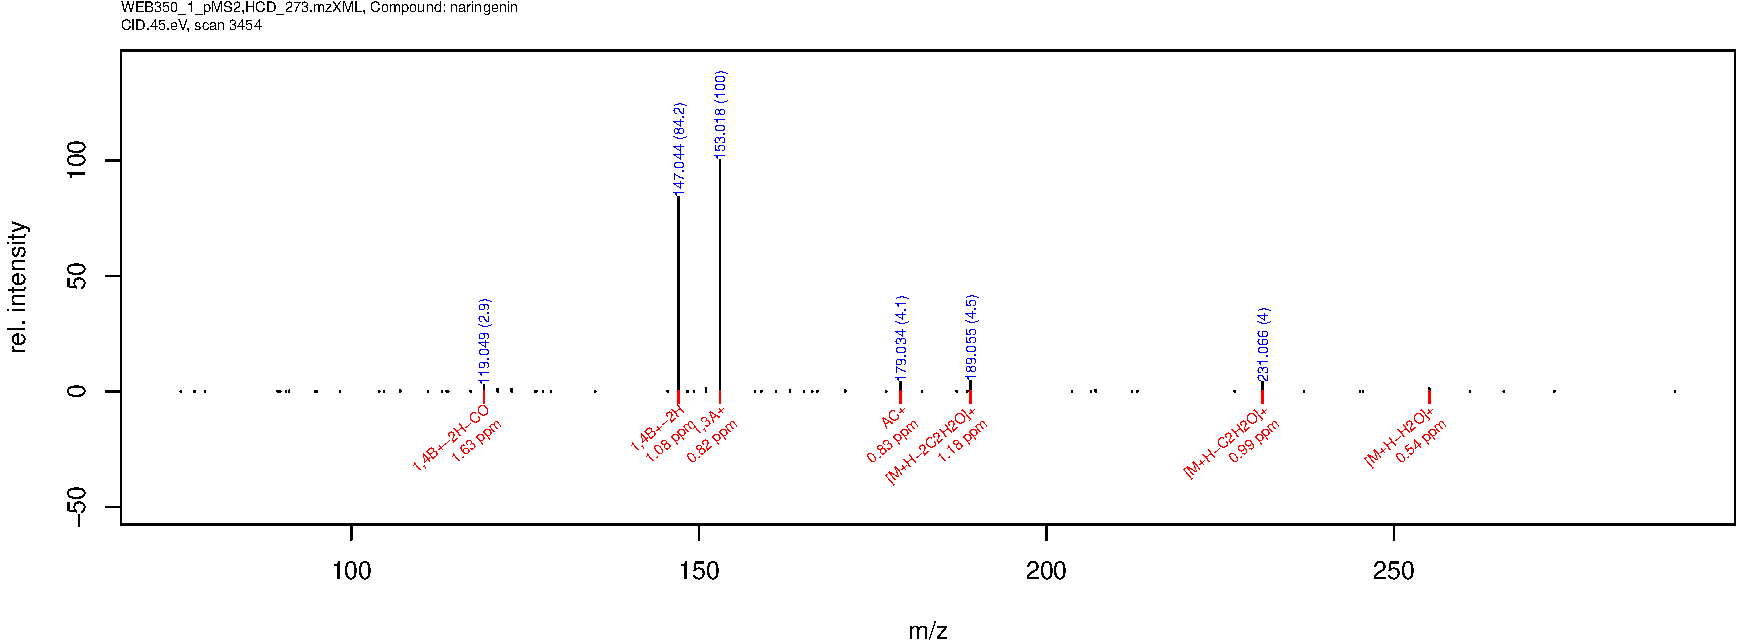
\includegraphics[width=\textwidth]{WEB350_files/figure-latex/unnamed-chunk-3-1}

\begin{table}[ht]
\centering
\begin{tabular}{rrrrl}
  \toprule
 & mz & int & ppm & fragment \\ 
  \midrule
1 & 119.05 & 2.9 & 1.63 & 1,4B+-2H-CO \\ 
  2 & 147.04 & 84.2 & 1.08 & 1,4B+-2H \\ 
  3 & 153.02 & 100.0 & 0.82 & 1,3A+ \\ 
  4 & 179.03 & 4.1 & 0.83 & AC+ \\ 
  5 & 189.05 & 4.5 & 1.18 & [M+H-2C2H2O]+ \\ 
  6 & 231.07 & 4.0 & 0.99 & [M+H-C2H2O]+ \\ 
  7 & 255.07 & 1.3 & 0.54 & [M+H-H2O]+ \\ 
   \bottomrule
\end{tabular}
\end{table}

\clearpage\subsection{naringenin.HCD.75eV}
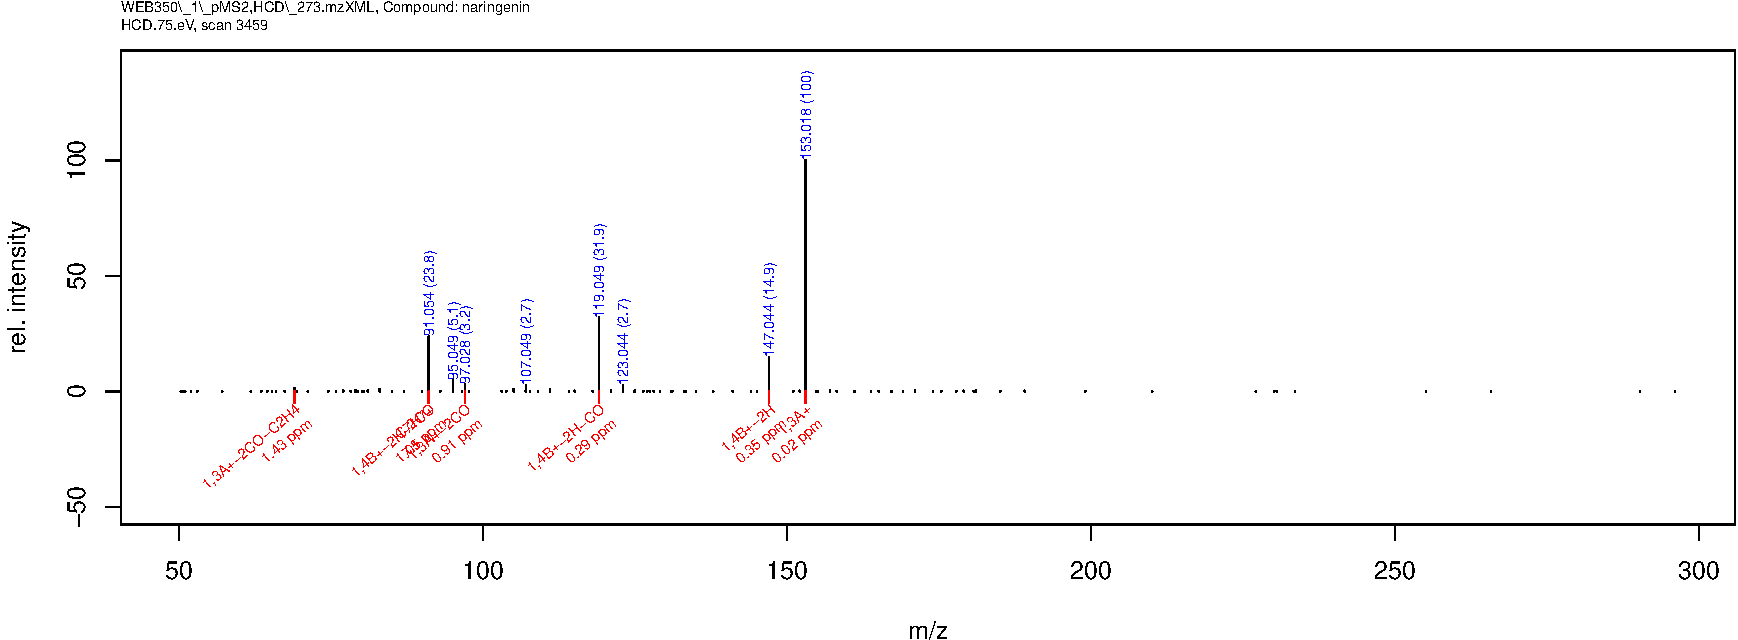
\includegraphics[width=\textwidth]{WEB350_files/figure-latex/unnamed-chunk-3-2}

\begin{table}[ht]
\centering
\begin{tabular}{rrrrl}
  \toprule
 & mz & int & ppm & fragment \\ 
  \midrule
1 & 69.00 & 1.5 & 1.43 & 1,3A+-2CO-C2H4 \\ 
  2 & 91.05 & 23.8 & 1.01 & 1,4B+-2H-2CO \\ 
  3 & 91.05 & 23.8 & 7.50 & C7H7+ \\ 
  4 & 97.03 & 3.2 & 0.91 & 1,3A+-2CO \\ 
  5 & 119.05 & 31.9 & 0.29 & 1,4B+-2H-CO \\ 
  6 & 147.04 & 14.9 & 0.35 & 1,4B+-2H \\ 
  7 & 153.02 & 100.0 & 0.02 & 1,3A+ \\ 
   \bottomrule
\end{tabular}
\end{table}

\clearpage\subsection{naringenin.HCD.100eV}
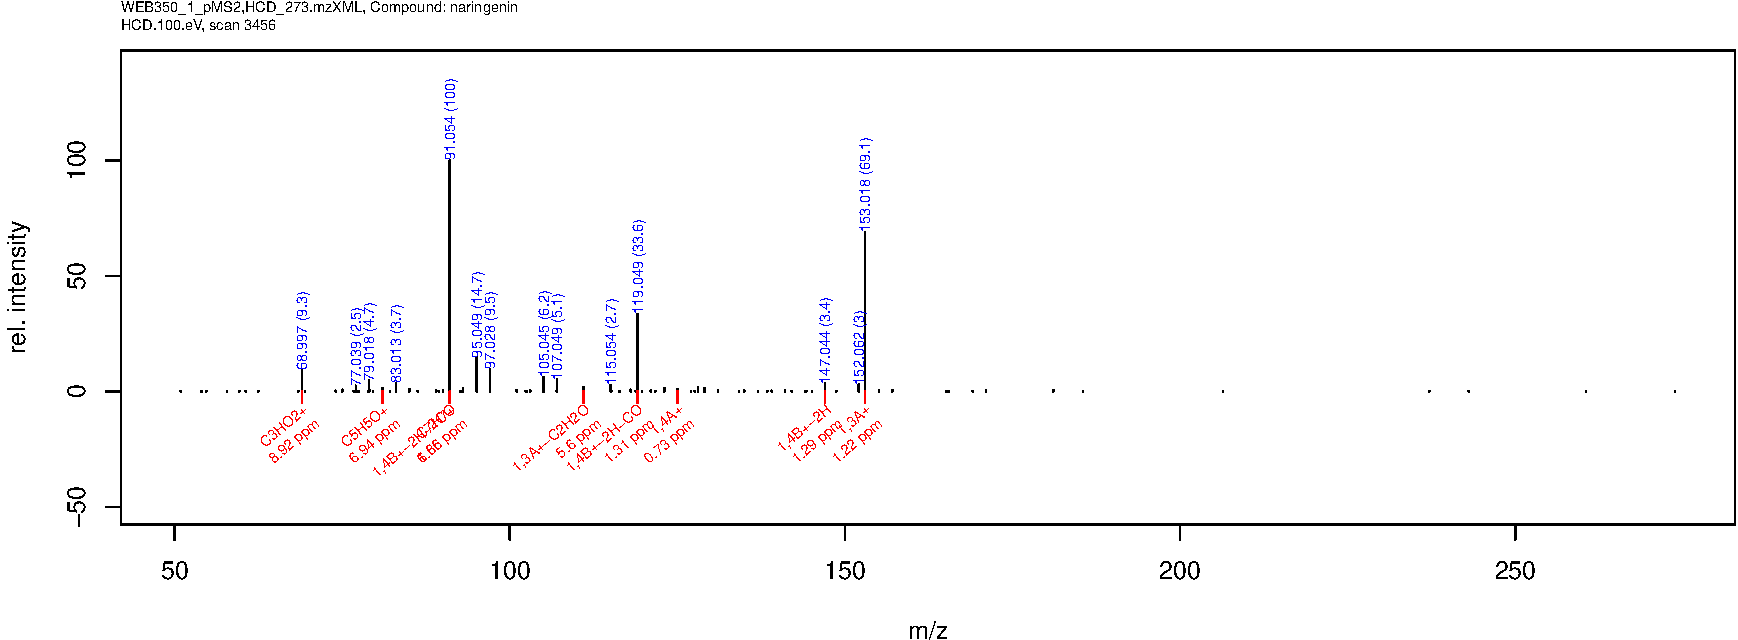
\includegraphics[width=\textwidth]{WEB350_files/figure-latex/unnamed-chunk-3-3}

\begin{table}[ht]
\centering
\begin{tabular}{rrrrl}
  \toprule
 & mz & int & ppm & fragment \\ 
  \midrule
1 & 69.00 & 9.3 & 0.44 & 1,3A+-2CO-C2H4 \\ 
  2 & 81.03 & 1.4 & 6.94 & C5H5O+ \\ 
  3 & 91.05 & 100.0 & 1.85 & 1,4B+-2H-2CO \\ 
  4 & 91.05 & 100.0 & 6.66 & C7H7+ \\ 
  5 & 97.03 & 9.5 & 0.04 & 1,3A+-2CO \\ 
  6 & 111.01 & 1.8 & 5.60 & 1,3A+-C2H2O \\ 
  7 & 119.05 & 33.6 & 1.31 & 1,4B+-2H-CO \\ 
  8 & 125.02 & 1.0 & 0.73 & 1,3A+-CO \\ 
  9 & 125.02 & 1.0 & 0.73 & 1,4A+ \\ 
  10 & 147.04 & 3.4 & 1.29 & 1,4B+-2H \\ 
  11 & 153.02 & 69.1 & 1.22 & 1,3A+ \\ 
   \bottomrule
\end{tabular}
\end{table}

\clearpage\subsection{eriodictyol.CID.45eV}
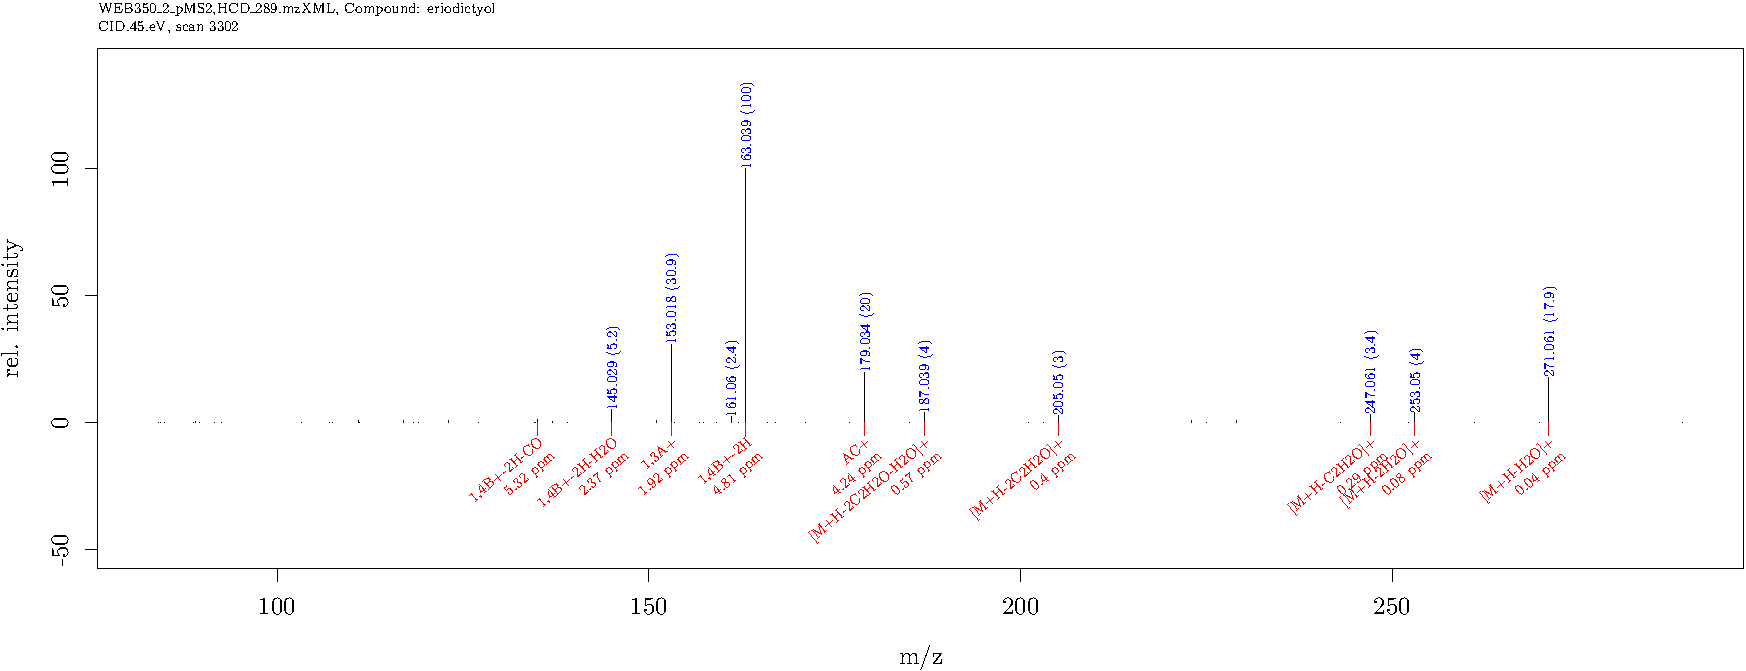
\includegraphics[width=\textwidth]{WEB350_files/figure-latex/unnamed-chunk-3-4}

\begin{table}[ht]
\centering
\begin{tabular}{rrrrl}
  \toprule
 & mz & int & ppm & fragment \\ 
  \midrule
1 & 135.04 & 1.1 & 5.32 & 1,4B+-2H-CO \\ 
  2 & 145.03 & 5.2 & 2.37 & 1,4B+-2H-H2O \\ 
  3 & 153.02 & 30.9 & 1.92 & 1,3A+ \\ 
  4 & 161.06 & 2.4 & 1.31 & [M+H-CH4-4CO]+ \\ 
  5 & 163.04 & 100.0 & 4.81 & 1,4B+-2H \\ 
  6 & 179.03 & 20.0 & 4.24 & AC+ \\ 
  7 & 187.04 & 4.0 & 0.57 & [M+H-2C2H2O-H2O]+ \\ 
  8 & 205.05 & 3.0 & 0.40 & [M+H-2C2H2O]+ \\ 
  9 & 247.06 & 3.4 & 0.29 & [M+H-C2H2O]+ \\ 
  10 & 253.05 & 4.0 & 0.08 & [M+H-2H2O]+ \\ 
  11 & 271.06 & 17.9 & 0.04 & [M+H-H2O]+ \\ 
   \bottomrule
\end{tabular}
\end{table}

\clearpage\subsection{eriodictyol.HCD.75eV}
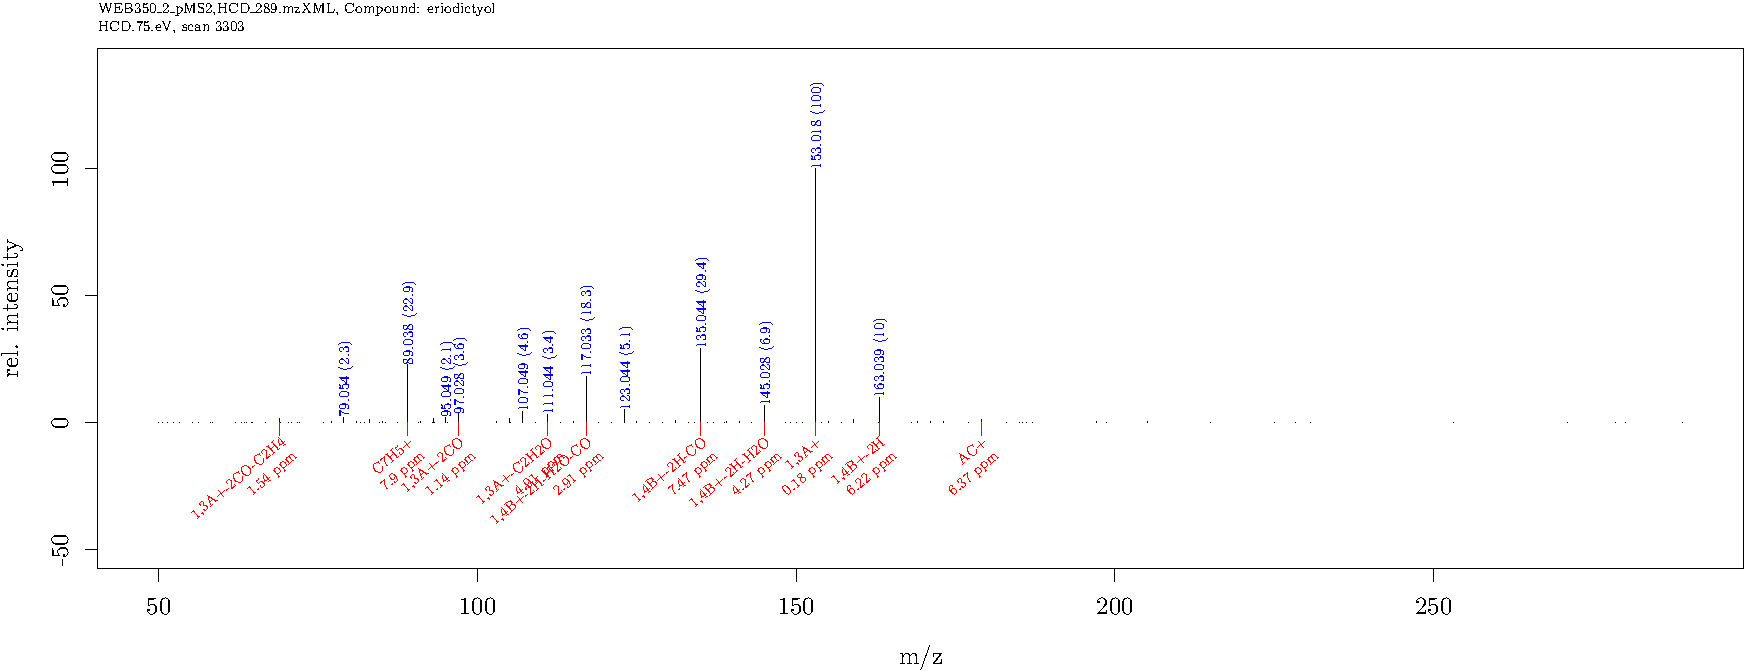
\includegraphics[width=\textwidth]{WEB350_files/figure-latex/unnamed-chunk-3-5}

\begin{table}[ht]
\centering
\begin{tabular}{rrrrl}
  \toprule
 & mz & int & ppm & fragment \\ 
  \midrule
1 & 69.00 & 1.7 & 1.54 & 1,3A+-2CO-C2H4 \\ 
  2 & 89.04 & 22.9 & 7.90 & C7H5+ \\ 
  3 & 97.03 & 3.6 & 1.14 & 1,3A+-2CO \\ 
  4 & 111.01 & 1.8 & 4.91 & 1,3A+-C2H2O \\ 
  5 & 117.03 & 18.3 & 2.91 & 1,4B+-2H-H2O-CO \\ 
  6 & 135.04 & 29.4 & 7.47 & 1,4B+-2H-CO \\ 
  7 & 145.03 & 6.9 & 4.27 & 1,4B+-2H-H2O \\ 
  8 & 153.02 & 100.0 & 0.18 & 1,3A+ \\ 
  9 & 163.04 & 10.0 & 6.22 & 1,4B+-2H \\ 
  10 & 179.03 & 1.1 & 6.37 & AC+ \\ 
   \bottomrule
\end{tabular}
\end{table}

\clearpage\subsection{eriodictyol.HCD.100eV}
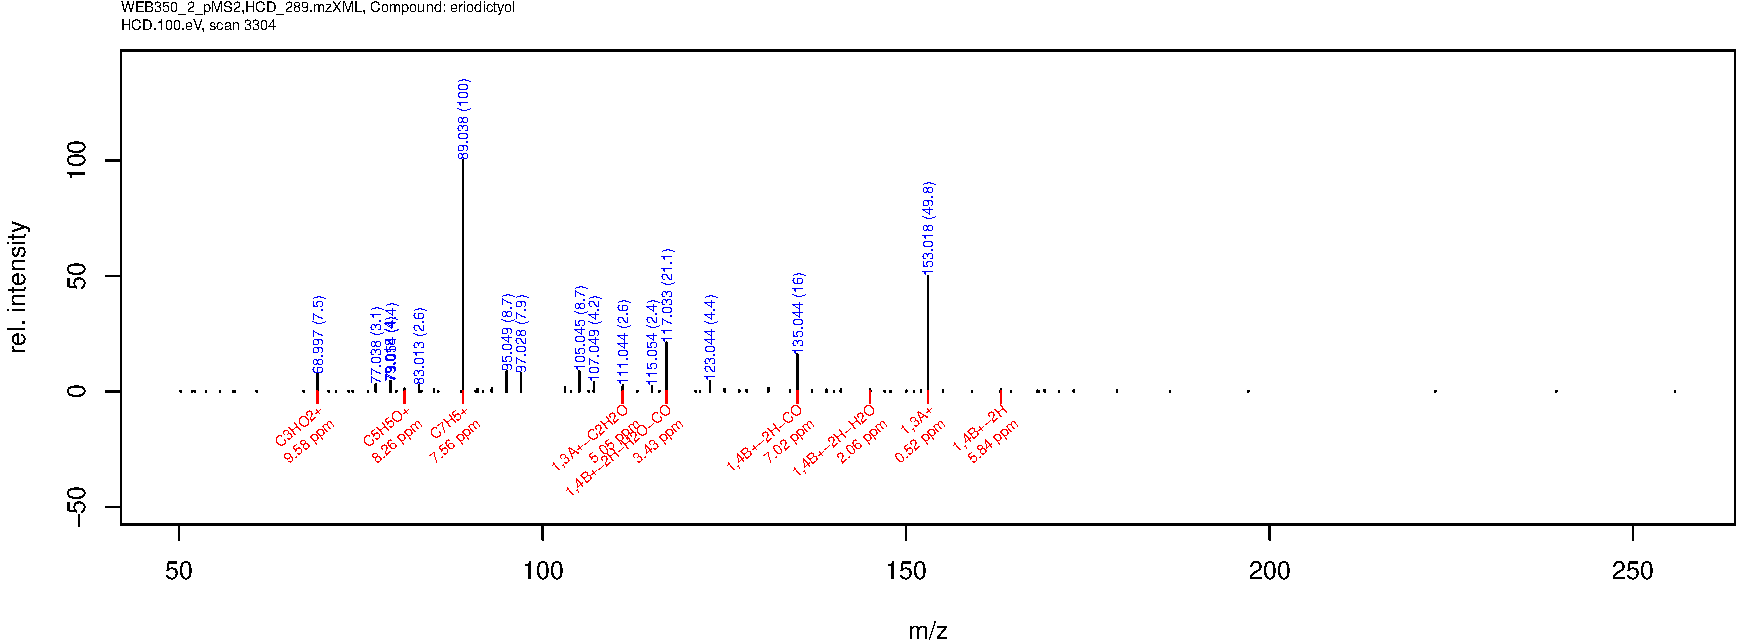
\includegraphics[width=\textwidth]{WEB350_files/figure-latex/unnamed-chunk-3-6}

\begin{table}[ht]
\centering
\begin{tabular}{rrrrl}
  \toprule
 & mz & int & ppm & fragment \\ 
  \midrule
1 & 69.00 & 7.5 & 1.10 & 1,3A+-2CO-C2H4 \\ 
  2 & 81.03 & 1.2 & 8.26 & C5H5O+ \\ 
  3 & 89.04 & 100.0 & 7.56 & C7H5+ \\ 
  4 & 97.03 & 7.9 & 0.75 & 1,3A+-2CO \\ 
  5 & 111.01 & 1.9 & 5.05 & 1,3A+-C2H2O \\ 
  6 & 117.03 & 21.1 & 3.43 & 1,4B+-2H-H2O-CO \\ 
  7 & 135.04 & 16.0 & 7.02 & 1,4B+-2H-CO \\ 
  8 & 145.03 & 1.0 & 2.06 & 1,4B+-2H-H2O \\ 
  9 & 153.02 & 49.8 & 0.52 & 1,3A+ \\ 
  10 & 163.04 & 1.0 & 5.84 & 1,4B+-2H \\ 
   \bottomrule
\end{tabular}
\end{table}

\clearpage\subsection{hesperetin.CID.45eV}
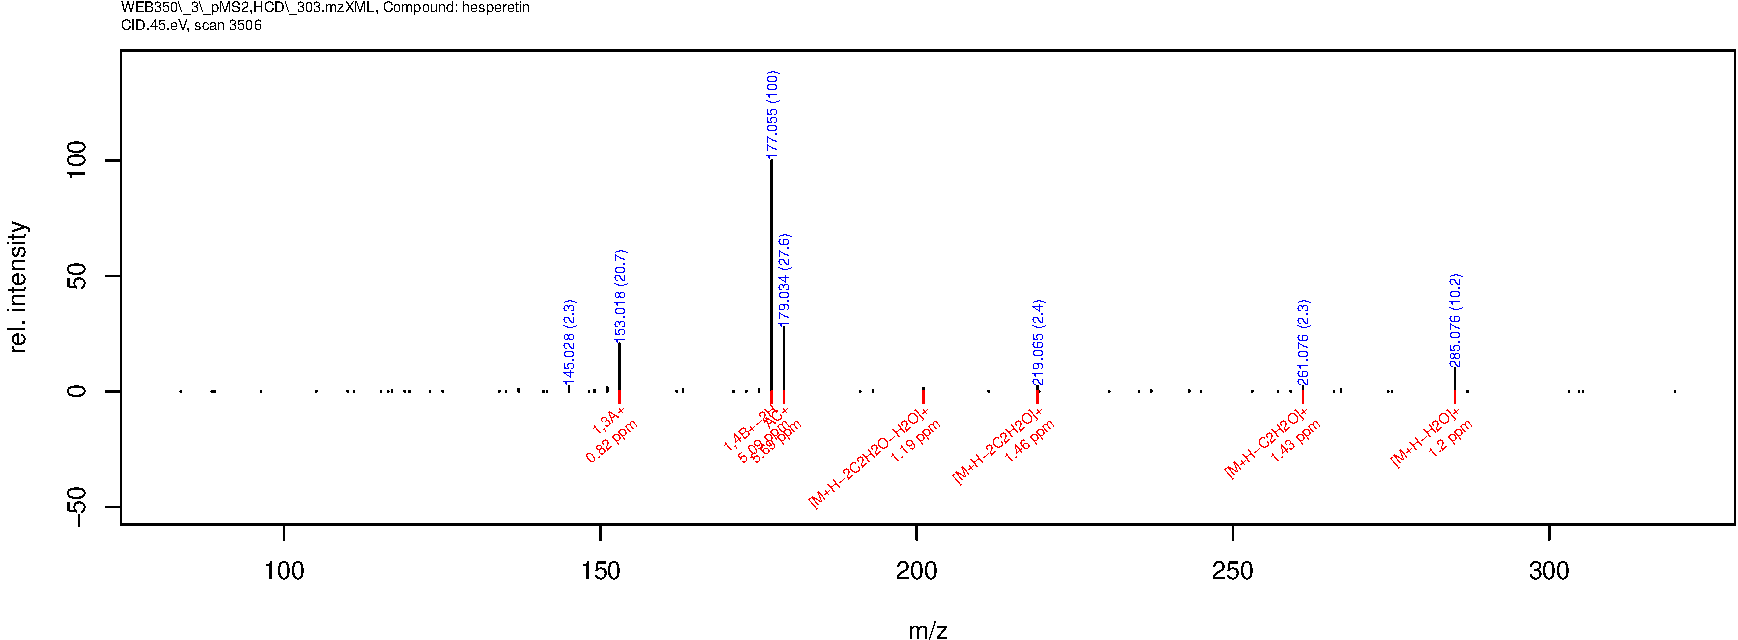
\includegraphics[width=\textwidth]{WEB350_files/figure-latex/unnamed-chunk-3-7}

\begin{table}[ht]
\centering
\begin{tabular}{rrrrl}
  \toprule
 & mz & int & ppm & fragment \\ 
  \midrule
1 & 153.02 & 20.7 & 0.82 & 1,3A+ \\ 
  2 & 177.05 & 100.0 & 5.09 & 1,4B+-2H \\ 
  3 & 179.03 & 27.6 & 5.69 & AC+ \\ 
  4 & 201.05 & 1.3 & 1.19 & [M+H-2C2H2O-H2O]+ \\ 
  5 & 219.07 & 2.4 & 1.46 & [M+H-2C2H2O]+ \\ 
  6 & 261.08 & 2.3 & 1.43 & [M+H-C2H2O]+ \\ 
  7 & 285.08 & 10.2 & 1.20 & [M+H-H2O]+ \\ 
   \bottomrule
\end{tabular}
\end{table}

\clearpage\subsection{hesperetin.HCD.75eV}
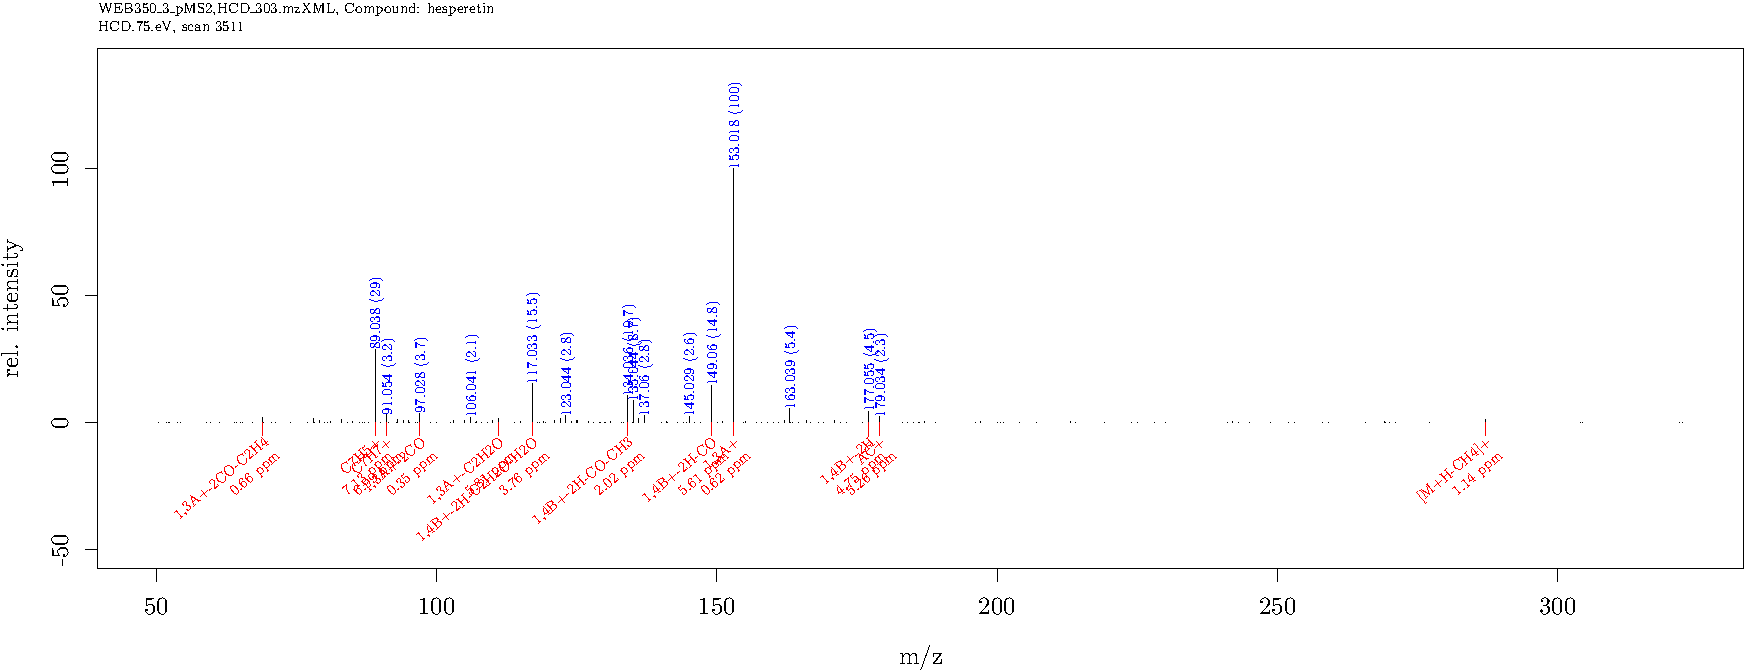
\includegraphics[width=\textwidth]{WEB350_files/figure-latex/unnamed-chunk-3-8}

\begin{table}[ht]
\centering
\begin{tabular}{rrrrl}
  \toprule
 & mz & int & ppm & fragment \\ 
  \midrule
1 & 69.00 & 2.0 & 0.66 & 1,3A+-2CO-C2H4 \\ 
  2 & 89.04 & 29.0 & 7.13 & C7H5+ \\ 
  3 & 91.05 & 3.2 & 6.99 & C7H7+ \\ 
  4 & 97.03 & 3.7 & 0.35 & 1,3A+-2CO \\ 
  5 & 111.01 & 1.4 & 5.81 & 1,3A+-C2H2O \\ 
  6 & 117.03 & 15.5 & 3.76 & 1,4B+-2H-C2H2O-H2O \\ 
  7 & 134.04 & 10.7 & 2.02 & 1,4B+-2H-CO-CH3 \\ 
  8 & 149.06 & 14.8 & 5.61 & 1,4B+-2H-CO \\ 
  9 & 153.02 & 100.0 & 0.62 & 1,3A+ \\ 
  10 & 177.05 & 4.5 & 4.75 & 1,4B+-2H \\ 
  11 & 179.03 & 2.3 & 5.26 & AC+ \\ 
  12 & 287.06 & 1.4 & 1.14 & [M+H-CH4]+ \\ 
   \bottomrule
\end{tabular}
\end{table}

\clearpage\subsection{hesperetin.HCD.100eV}
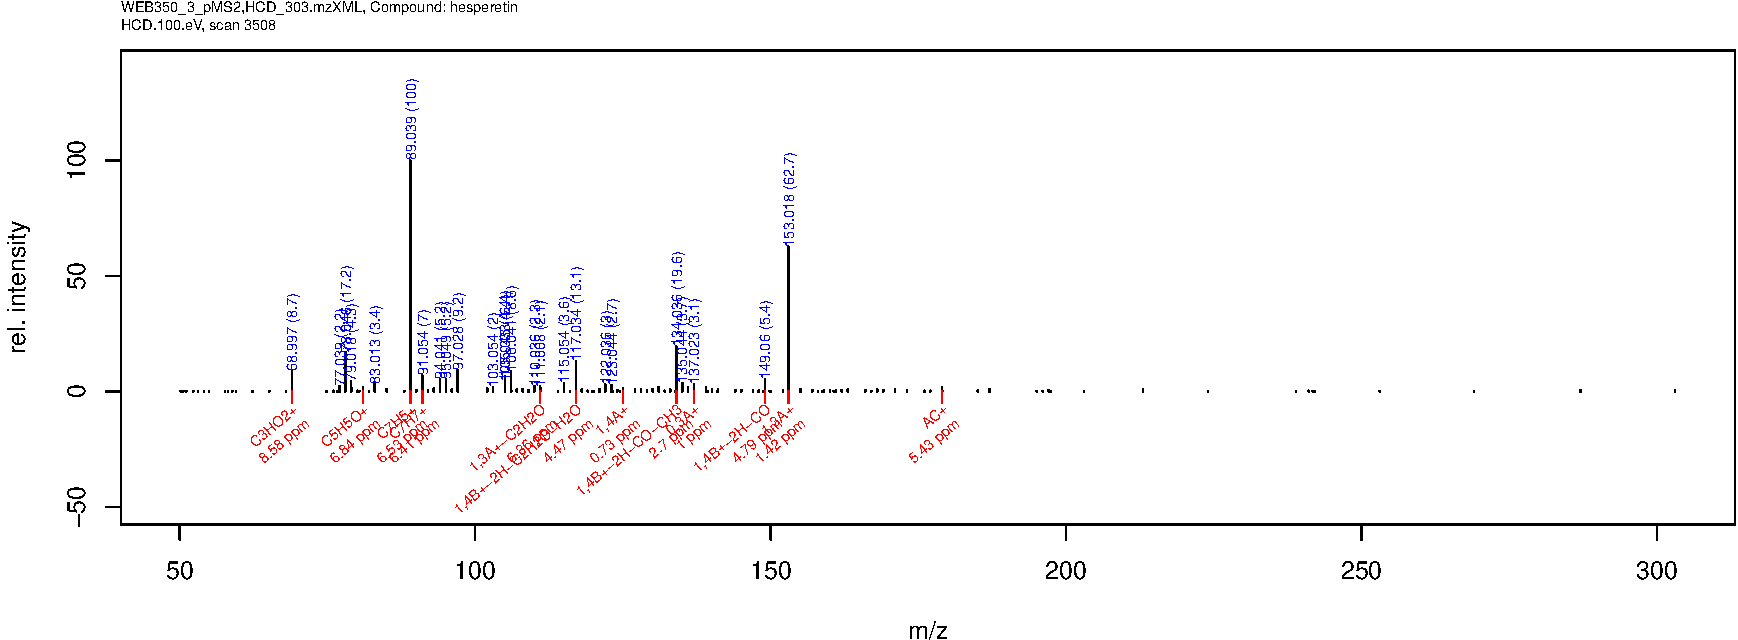
\includegraphics[width=\textwidth]{WEB350_files/figure-latex/unnamed-chunk-3-9}

\begin{table}[ht]
\centering
\begin{tabular}{rrrrl}
  \toprule
 & mz & int & ppm & fragment \\ 
  \midrule
1 & 69.00 & 8.7 & 0.11 & 1,3A+-2CO-C2H4 \\ 
  2 & 81.03 & 1.9 & 6.84 & C5H5O+ \\ 
  3 & 89.04 & 100.0 & 6.53 & C7H5+ \\ 
  4 & 91.05 & 7.0 & 6.41 & C7H7+ \\ 
  5 & 97.03 & 9.2 & 0.35 & 1,3A+-2CO \\ 
  6 & 111.01 & 2.1 & 6.36 & 1,3A+-C2H2O \\ 
  7 & 117.03 & 13.1 & 4.47 & 1,4B+-2H-C2H2O-H2O \\ 
  8 & 125.02 & 1.2 & 0.73 & 1,3A+-CO \\ 
  9 & 125.02 & 1.2 & 0.73 & 1,4A+ \\ 
  10 & 134.04 & 19.6 & 2.70 & 1,4B+-2H-CO-CH3 \\ 
  11 & 137.02 & 3.1 & 1.00 & 0,3A+ \\ 
  12 & 149.06 & 5.4 & 4.79 & 1,4B+-2H-CO \\ 
  13 & 153.02 & 62.7 & 1.42 & 1,3A+ \\ 
  14 & 179.03 & 1.6 & 5.43 & AC+ \\ 
   \bottomrule
\end{tabular}
\end{table}

\clearpage\subsection{homoeriodictyol.CID.45eV}
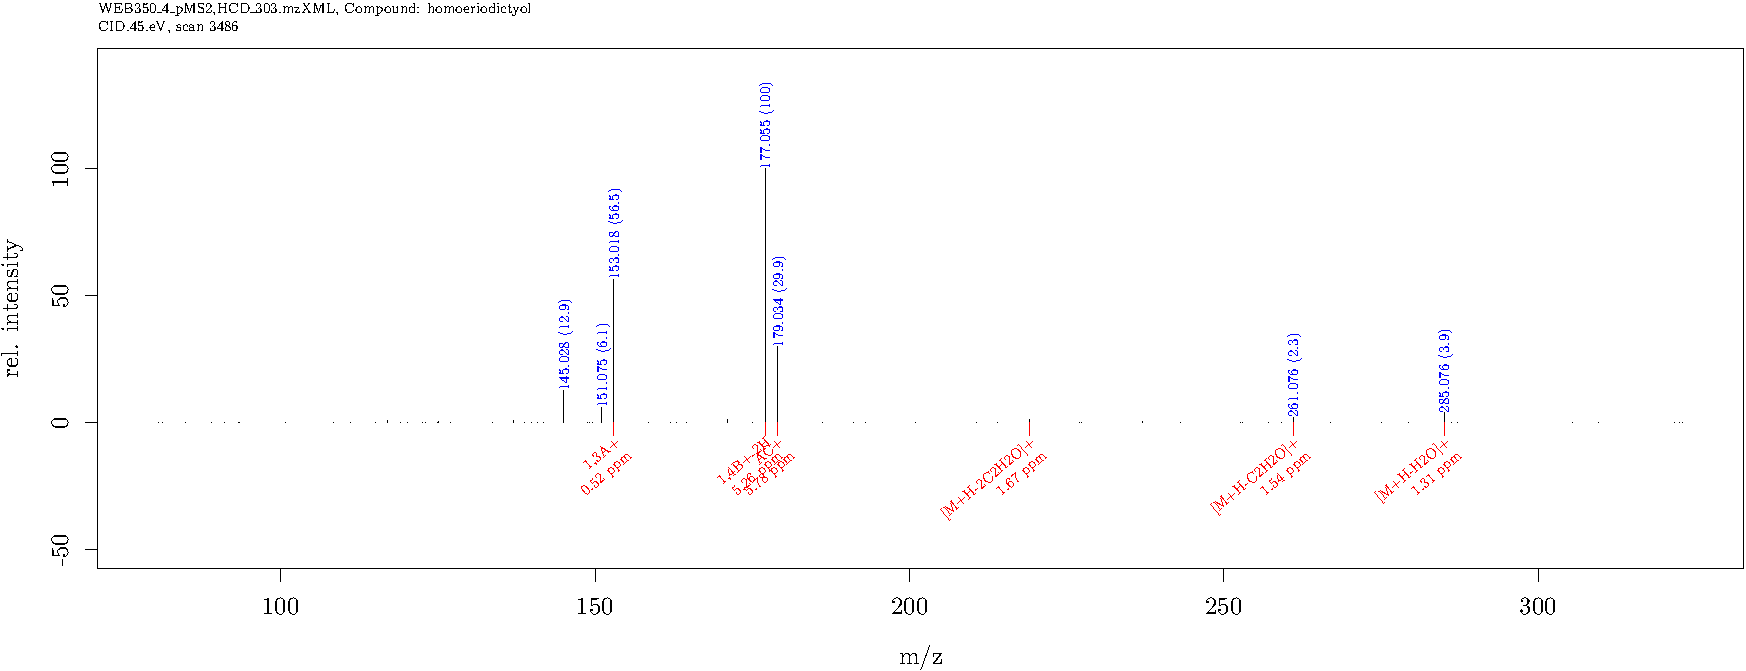
\includegraphics[width=\textwidth]{WEB350_files/figure-latex/unnamed-chunk-3-10}

\begin{table}[ht]
\centering
\begin{tabular}{rrrrl}
  \toprule
 & mz & int & ppm & fragment \\ 
  \midrule
1 & 153.02 & 56.5 & 0.52 & 1,3A+ \\ 
  2 & 177.05 & 100.0 & 5.26 & 1,4B+-2H \\ 
  3 & 179.03 & 29.9 & 5.78 & AC+ \\ 
  4 & 219.07 & 1.4 & 1.67 & [M+H-2C2H2O]+ \\ 
  5 & 261.08 & 2.3 & 1.54 & [M+H-C2H2O]+ \\ 
  6 & 285.08 & 3.9 & 1.31 & [M+H-H2O]+ \\ 
   \bottomrule
\end{tabular}
\end{table}

\clearpage\subsection{homoeriodictyol.HCD.75eV}
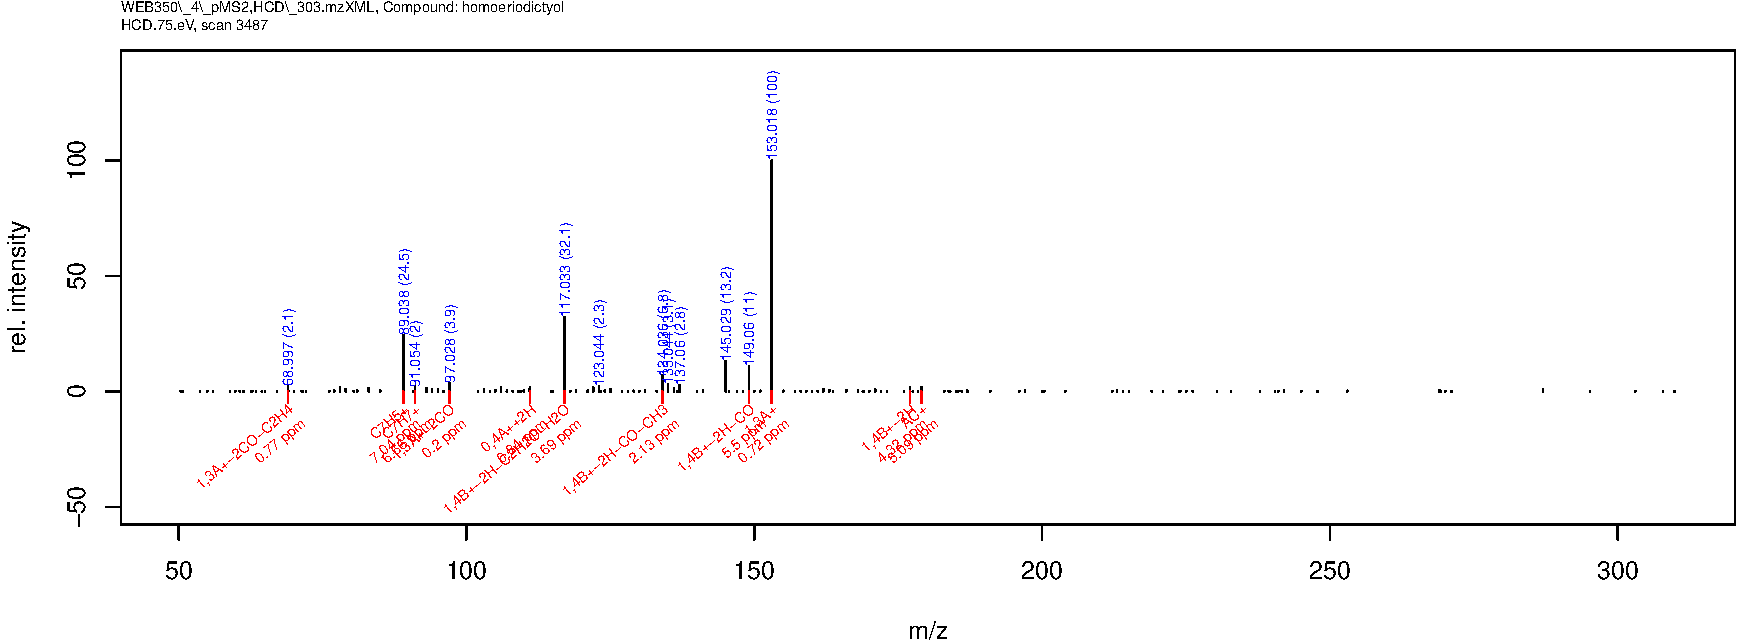
\includegraphics[width=\textwidth]{WEB350_files/figure-latex/unnamed-chunk-3-11}

\begin{table}[ht]
\centering
\begin{tabular}{rrrrl}
  \toprule
 & mz & int & ppm & fragment \\ 
  \midrule
1 & 69.00 & 2.1 & 0.77 & 1,3A+-2CO-C2H4 \\ 
  2 & 89.04 & 24.5 & 7.04 & C7H5+ \\ 
  3 & 91.05 & 2.0 & 6.66 & C7H7+ \\ 
  4 & 97.03 & 3.9 & 0.20 & 1,3A+-2CO \\ 
  5 & 111.04 & 1.8 & 0.84 & 0,4A++2H \\ 
  6 & 117.03 & 32.1 & 3.69 & 1,4B+-2H-C2H2O-H2O \\ 
  7 & 134.04 & 6.8 & 2.13 & 1,4B+-2H-CO-CH3 \\ 
  8 & 149.06 & 11.0 & 5.50 & 1,4B+-2H-CO \\ 
  9 & 153.02 & 100.0 & 0.72 & 1,3A+ \\ 
  10 & 177.05 & 1.8 & 4.32 & 1,4B+-2H \\ 
  11 & 179.03 & 1.8 & 5.09 & AC+ \\ 
   \bottomrule
\end{tabular}
\end{table}

\clearpage\subsection{homoeriodictyol.HCD.100eV}
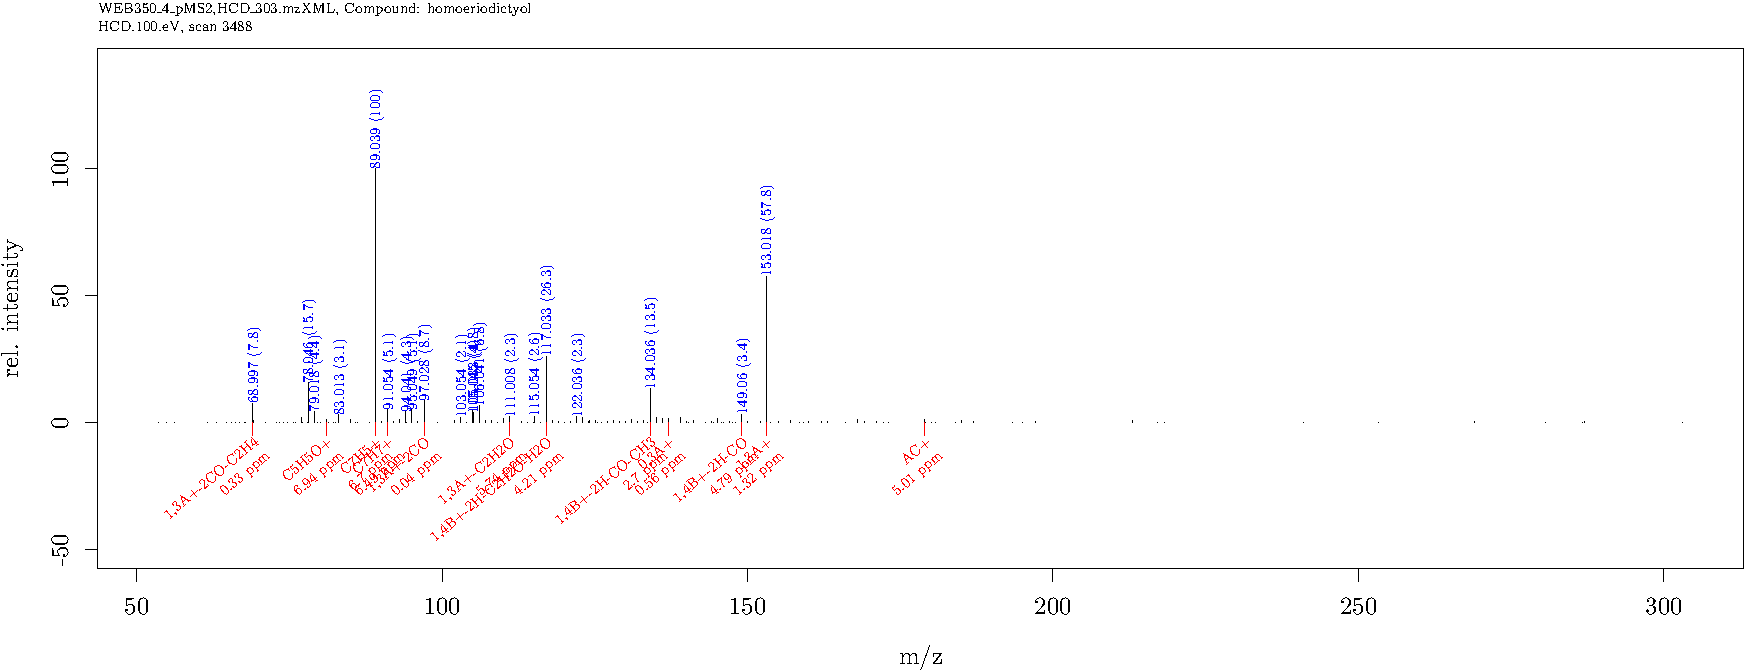
\includegraphics[width=\textwidth]{WEB350_files/figure-latex/unnamed-chunk-3-12}

\begin{table}[ht]
\centering
\begin{tabular}{rrrrl}
  \toprule
 & mz & int & ppm & fragment \\ 
  \midrule
1 & 69.00 & 7.8 & 0.33 & 1,3A+-2CO-C2H4 \\ 
  2 & 81.03 & 1.2 & 6.94 & C5H5O+ \\ 
  3 & 89.04 & 100.0 & 6.70 & C7H5+ \\ 
  4 & 91.05 & 5.1 & 6.49 & C7H7+ \\ 
  5 & 97.03 & 8.7 & 0.04 & 1,3A+-2CO \\ 
  6 & 111.01 & 2.3 & 5.74 & 1,3A+-C2H2O \\ 
  7 & 117.03 & 26.3 & 4.21 & 1,4B+-2H-C2H2O-H2O \\ 
  8 & 134.04 & 13.5 & 2.70 & 1,4B+-2H-CO-CH3 \\ 
  9 & 137.02 & 1.8 & 0.56 & 0,3A+ \\ 
  10 & 149.06 & 3.4 & 4.79 & 1,4B+-2H-CO \\ 
  11 & 153.02 & 57.8 & 1.32 & 1,3A+ \\ 
  12 & 179.03 & 1.1 & 5.01 & AC+ \\ 
   \bottomrule
\end{tabular}
\end{table}

\clearpage\subsection{apigenin.CID.45eV}
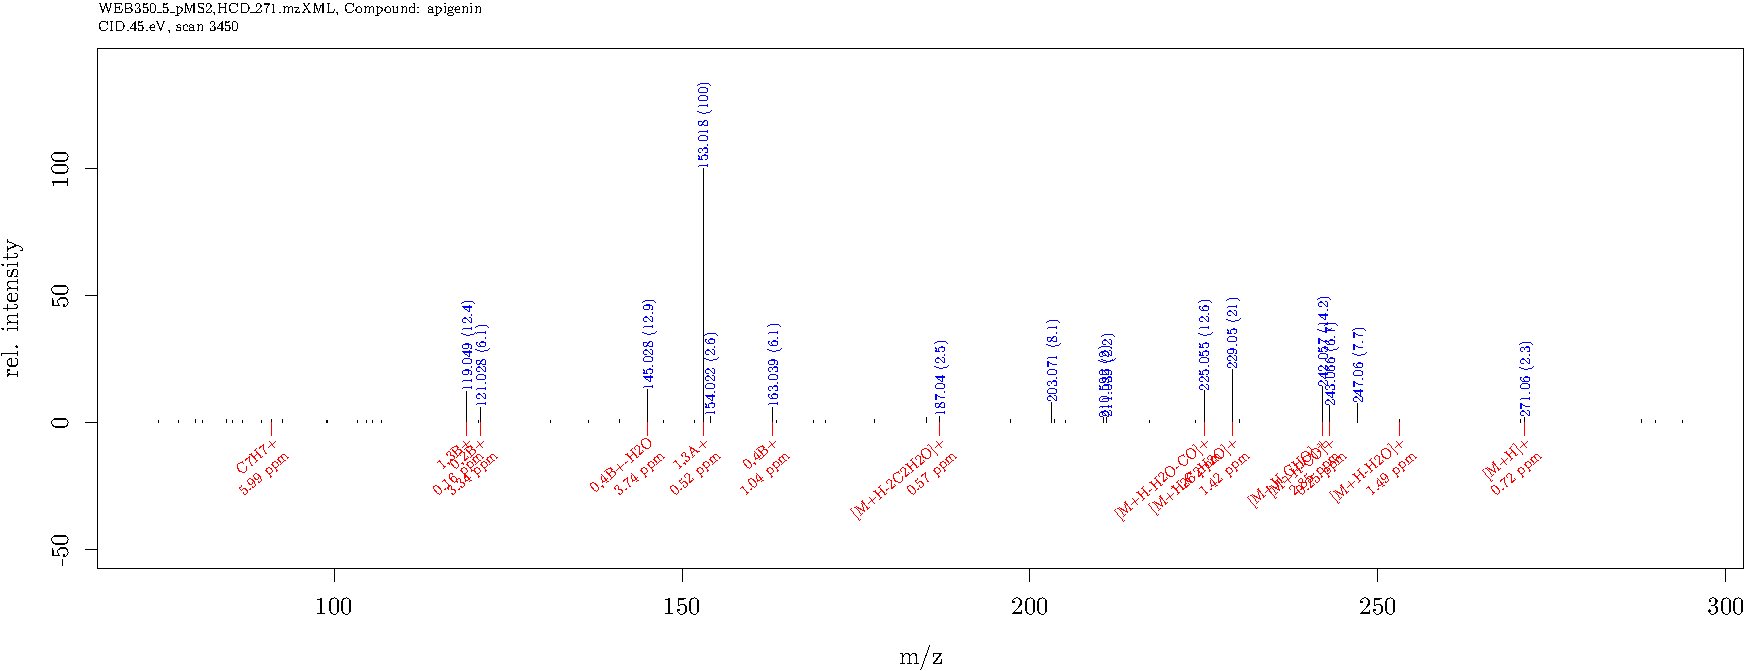
\includegraphics[width=\textwidth]{WEB350_files/figure-latex/unnamed-chunk-3-13}

\begin{table}[ht]
\centering
\begin{tabular}{rrrrl}
  \toprule
 & mz & int & ppm & fragment \\ 
  \midrule
1 & 91.05 & 1.2 & 5.99 & C7H7+ \\ 
  2 & 119.05 & 12.4 & 0.16 & 1,3B+ \\ 
  3 & 121.03 & 6.1 & 3.34 & 0,2B+ \\ 
  4 & 145.03 & 12.9 & 3.74 & 0,4B+-H2O \\ 
  5 & 153.02 & 100.0 & 0.52 & 1,3A+ \\ 
  6 & 163.04 & 6.1 & 1.04 & 0,4B+ \\ 
  7 & 187.04 & 2.5 & 0.57 & [M+H-2C2H2O]+ \\ 
  8 & 225.05 & 12.6 & 1.26 & [M+H-H2O-CO]+ \\ 
  9 & 229.05 & 21.0 & 1.42 & [M+H-C2H2O]+ \\ 
  10 & 242.06 & 14.2 & 2.85 & [M+H-CHO].+ \\ 
  11 & 243.07 & 6.7 & 0.25 & [M+H-CO]+ \\ 
  12 & 253.05 & 1.3 & 1.49 & [M+H-H2O]+ \\ 
  13 & 271.06 & 2.3 & 0.72 & [M+H]+ \\ 
   \bottomrule
\end{tabular}
\end{table}

\clearpage\subsection{apigenin.HCD.75eV}
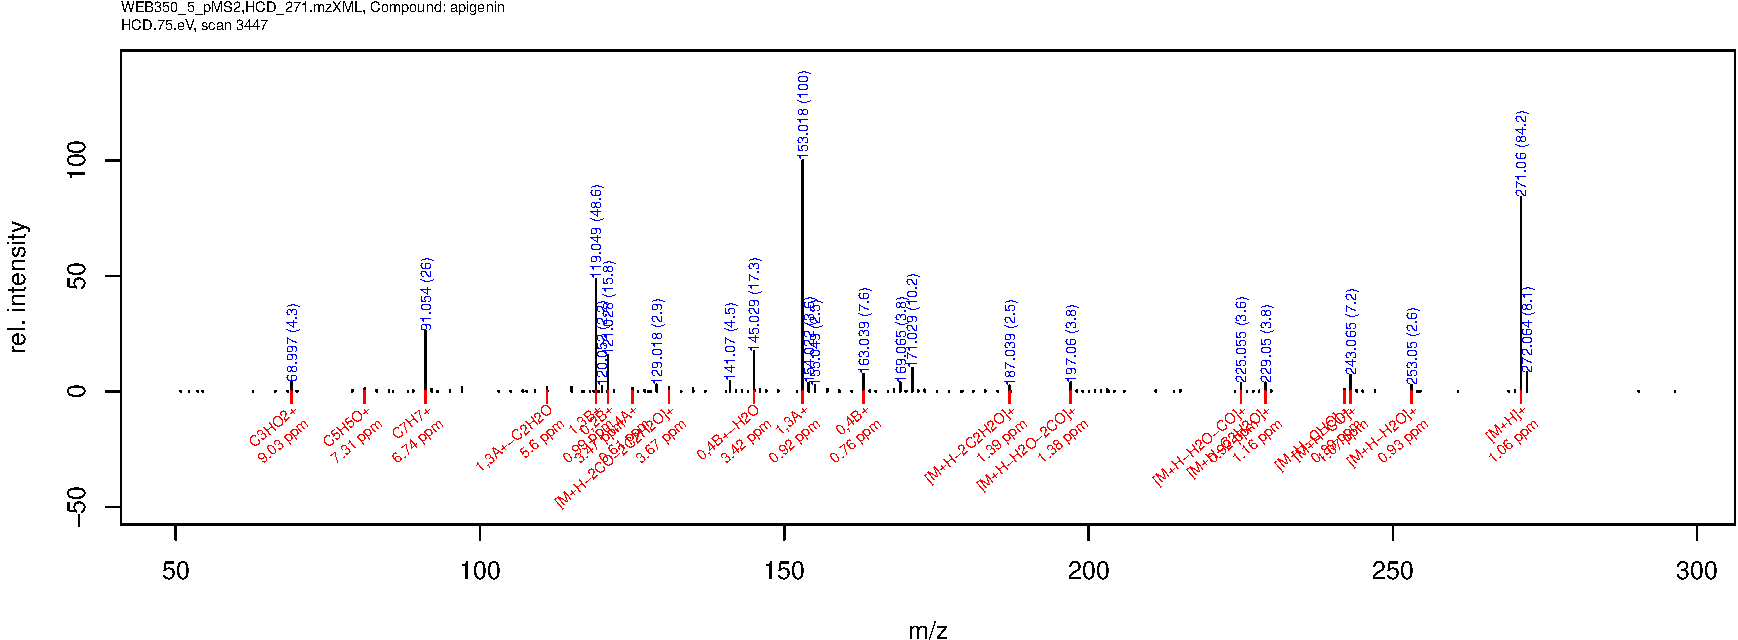
\includegraphics[width=\textwidth]{WEB350_files/figure-latex/unnamed-chunk-3-14}

\begin{table}[ht]
\centering
\begin{tabular}{rrrrl}
  \toprule
 & mz & int & ppm & fragment \\ 
  \midrule
1 & 69.00 & 4.3 & 0.55 & 1,3A+-2CO-C2H4 \\ 
  2 & 81.03 & 1.2 & 7.31 & C5H5O+ \\ 
  3 & 91.05 & 26.0 & 6.74 & C7H7+ \\ 
  4 & 97.03 & 1.8 & 0.43 & 1,3A+-2CO \\ 
  5 & 111.01 & 2.0 & 5.60 & 1,3A+-C2H2O \\ 
  6 & 119.05 & 48.6 & 0.99 & 1,3B+ \\ 
  7 & 121.03 & 15.8 & 3.47 & 0,2B+ \\ 
  8 & 125.02 & 1.5 & 0.61 & 1,3A+-CO \\ 
  9 & 125.02 & 1.5 & 0.61 & 1,4A+ \\ 
  10 & 131.05 & 1.7 & 3.67 & [M+H-2CO-2C2H2O]+ \\ 
  11 & 145.03 & 17.3 & 3.42 & 0,4B+-H2O \\ 
  12 & 153.02 & 100.0 & 0.92 & 1,3A+ \\ 
  13 & 163.04 & 7.6 & 0.76 & 0,4B+ \\ 
  14 & 187.04 & 2.5 & 1.39 & [M+H-2C2H2O]+ \\ 
  15 & 197.06 & 3.8 & 1.38 & [M+H-H2O-2CO]+ \\ 
  16 & 225.05 & 3.6 & 0.92 & [M+H-H2O-CO]+ \\ 
  17 & 229.05 & 3.8 & 1.16 & [M+H-C2H2O]+ \\ 
  18 & 242.06 & 1.0 & 0.89 & [M+H-CHO].+ \\ 
  19 & 243.07 & 7.2 & 1.07 & [M+H-CO]+ \\ 
  20 & 253.05 & 2.6 & 0.93 & [M+H-H2O]+ \\ 
  21 & 271.06 & 84.2 & 1.06 & [M+H]+ \\ 
   \bottomrule
\end{tabular}
\end{table}

\clearpage\subsection{apigenin.HCD.100eV}
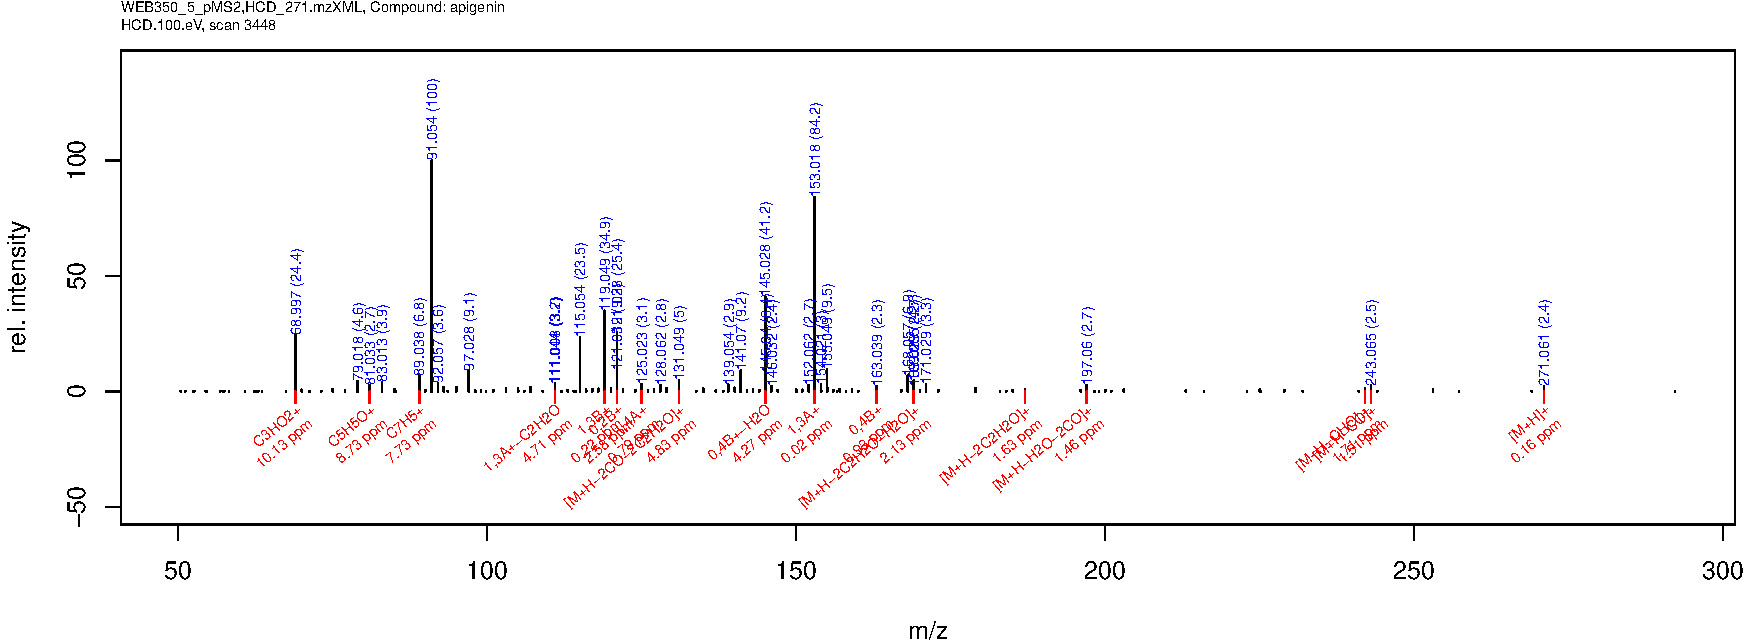
\includegraphics[width=\textwidth]{WEB350_files/figure-latex/unnamed-chunk-3-15}

\begin{table}[ht]
\centering
\begin{tabular}{rrrrl}
  \toprule
 & mz & int & ppm & fragment \\ 
  \midrule
1 & 69.00 & 24.4 & 1.65 & 1,3A+-2CO-C2H4 \\ 
  2 & 81.03 & 2.7 & 8.73 & C5H5O+ \\ 
  3 & 89.04 & 6.8 & 7.73 & C7H5+ \\ 
  4 & 97.03 & 9.1 & 1.06 & 1,3A+-2CO \\ 
  5 & 111.01 & 3.7 & 4.71 & 1,3A+-C2H2O \\ 
  6 & 119.05 & 34.9 & 0.22 & 1,3B+ \\ 
  7 & 121.03 & 25.4 & 2.58 & 0,2B+ \\ 
  8 & 125.02 & 3.1 & 0.79 & 1,3A+-CO \\ 
  9 & 125.02 & 3.1 & 0.79 & 1,4A+ \\ 
  10 & 131.05 & 5.0 & 4.83 & [M+H-2CO-2C2H2O]+ \\ 
  11 & 143.05 & 1.1 & 2.61 & [M+H-CH4-4CO]+ \\ 
  12 & 145.03 & 41.2 & 4.27 & 0,4B+-H2O \\ 
  13 & 153.02 & 84.2 & 0.02 & 1,3A+ \\ 
  14 & 163.04 & 2.3 & 0.93 & 0,4B+ \\ 
  15 & 169.03 & 2.2 & 2.13 & [M+H-2C2H2O-H2O]+ \\ 
  16 & 187.04 & 1.0 & 1.63 & [M+H-2C2H2O]+ \\ 
  17 & 197.06 & 2.7 & 1.46 & [M+H-H2O-2CO]+ \\ 
  18 & 242.06 & 1.5 & 1.71 & [M+H-CHO].+ \\ 
  19 & 243.07 & 2.5 & 1.51 & [M+H-CO]+ \\ 
  20 & 271.06 & 2.4 & 0.16 & [M+H]+ \\ 
   \bottomrule
\end{tabular}
\end{table}

\clearpage\subsection{luteolin.CID.45eV}
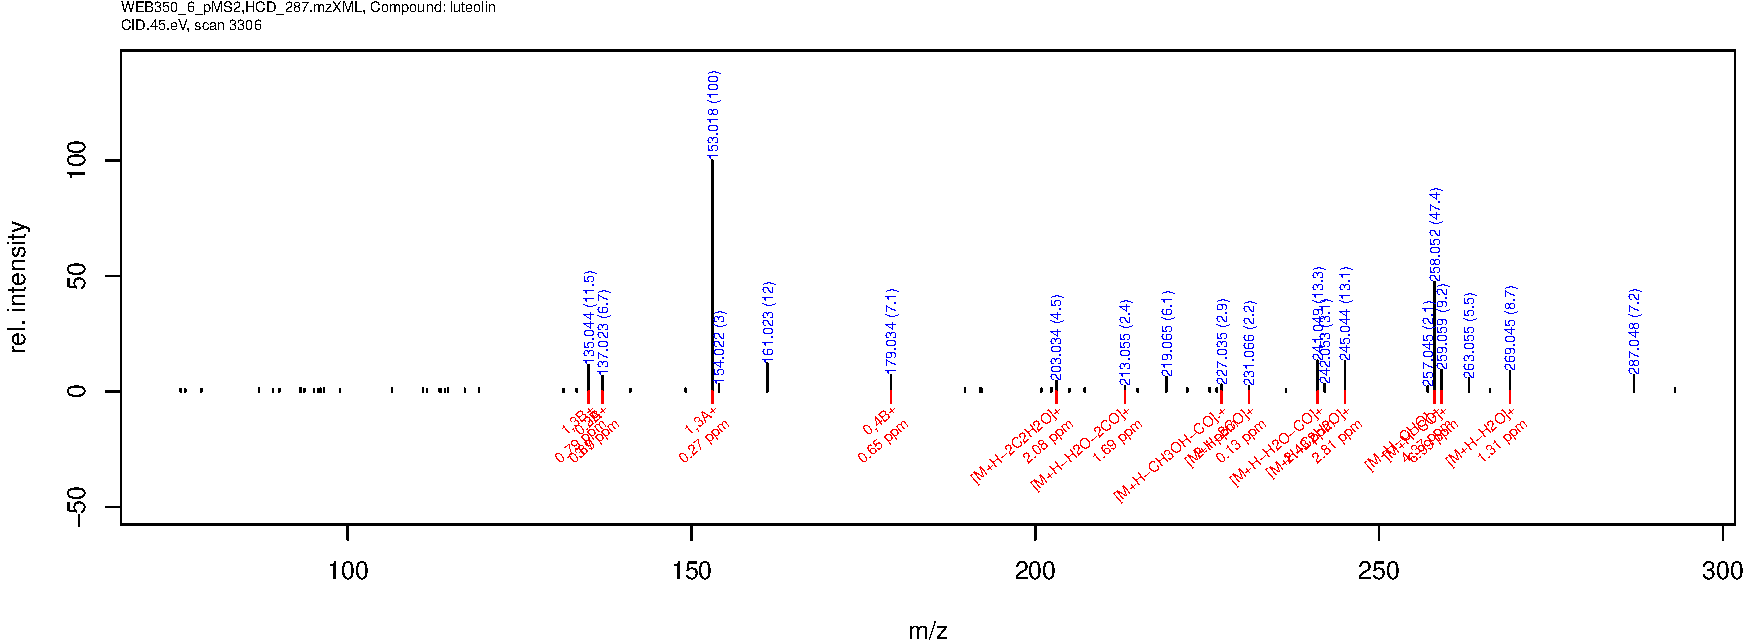
\includegraphics[width=\textwidth]{WEB350_files/figure-latex/unnamed-chunk-3-16}

\begin{table}[ht]
\centering
\begin{tabular}{rrrrl}
  \toprule
 & mz & int & ppm & fragment \\ 
  \midrule
1 & 135.04 & 11.5 & 0.79 & 1,3B+ \\ 
  2 & 137.02 & 6.7 & 3.70 & 0,2B+ \\ 
  3 & 137.02 & 6.7 & 0.89 & 0,3A+ \\ 
  4 & 153.02 & 100.0 & 0.27 & 1,3A+ \\ 
  5 & 179.03 & 7.1 & 0.65 & 0,4B+ \\ 
  6 & 203.03 & 4.5 & 2.08 & [M+H-2C2H2O]+ \\ 
  7 & 213.05 & 2.4 & 1.69 & [M+H-H2O-2CO]+ \\ 
  8 & 227.03 & 2.9 & 2.10 & [M+H-CH3OH-CO].+ \\ 
  9 & 231.07 & 2.2 & 0.13 & [M+H-2CO]+ \\ 
  10 & 241.05 & 13.3 & 2.43 & [M+H-H2O-CO]+ \\ 
  11 & 245.04 & 13.1 & 2.81 & [M+H-C2H2O]+ \\ 
  12 & 258.05 & 47.4 & 4.37 & [M+H-CHO].+ \\ 
  13 & 259.06 & 9.2 & 6.99 & [M+H-CO]+ \\ 
  14 & 269.04 & 8.7 & 1.31 & [M+H-H2O]+ \\ 
   \bottomrule
\end{tabular}
\end{table}

\clearpage\subsection{luteolin.HCD.75eV}
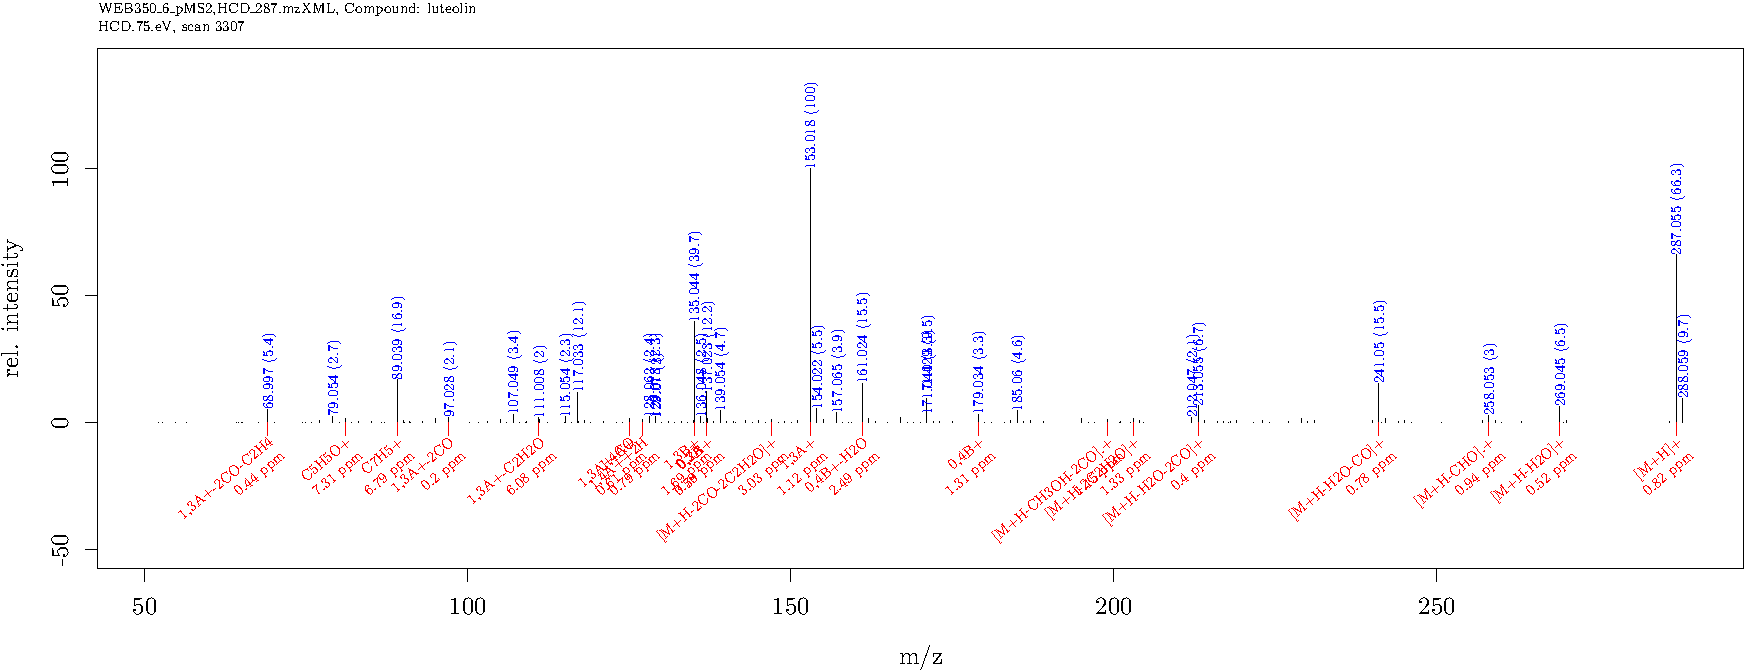
\includegraphics[width=\textwidth]{WEB350_files/figure-latex/unnamed-chunk-3-17}

\begin{table}[ht]
\centering
\begin{tabular}{rrrrl}
  \toprule
 & mz & int & ppm & fragment \\ 
  \midrule
1 & 69.00 & 5.4 & 0.44 & 1,3A+-2CO-C2H4 \\ 
  2 & 81.03 & 1.6 & 7.31 & C5H5O+ \\ 
  3 & 89.04 & 16.9 & 6.79 & C7H5+ \\ 
  4 & 97.03 & 2.1 & 0.20 & 1,3A+-2CO \\ 
  5 & 111.01 & 2.0 & 6.08 & 1,3A+-C2H2O \\ 
  6 & 125.02 & 1.7 & 0.61 & 1,3A+-CO \\ 
  7 & 125.02 & 1.7 & 0.61 & 1,4A+ \\ 
  8 & 127.04 & 1.2 & 0.79 & 1,4A++2H \\ 
  9 & 135.04 & 39.7 & 1.69 & 1,3B+ \\ 
  10 & 137.02 & 12.2 & 3.59 & 0,2B+ \\ 
  11 & 137.02 & 12.2 & 0.78 & 0,3A+ \\ 
  12 & 147.04 & 1.5 & 3.03 & [M+H-2CO-2C2H2O]+ \\ 
  13 & 153.02 & 100.0 & 1.12 & 1,3A+ \\ 
  14 & 161.02 & 15.5 & 2.49 & 0,4B+-H2O \\ 
  15 & 179.03 & 3.3 & 1.31 & 0,4B+ \\ 
  16 & 199.04 & 1.4 & 1.15 & [M+H-CH3OH-2CO].+ \\ 
  17 & 203.03 & 1.7 & 1.33 & [M+H-2C2H2O]+ \\ 
  18 & 213.06 & 6.7 & 0.40 & [M+H-H2O-2CO]+ \\ 
  19 & 241.05 & 15.5 & 0.78 & [M+H-H2O-CO]+ \\ 
  20 & 258.05 & 3.0 & 0.94 & [M+H-CHO].+ \\ 
  21 & 269.04 & 6.5 & 0.52 & [M+H-H2O]+ \\ 
  22 & 287.06 & 66.3 & 0.82 & [M+H]+ \\ 
   \bottomrule
\end{tabular}
\end{table}

\clearpage\subsection{luteolin.HCD.100eV}
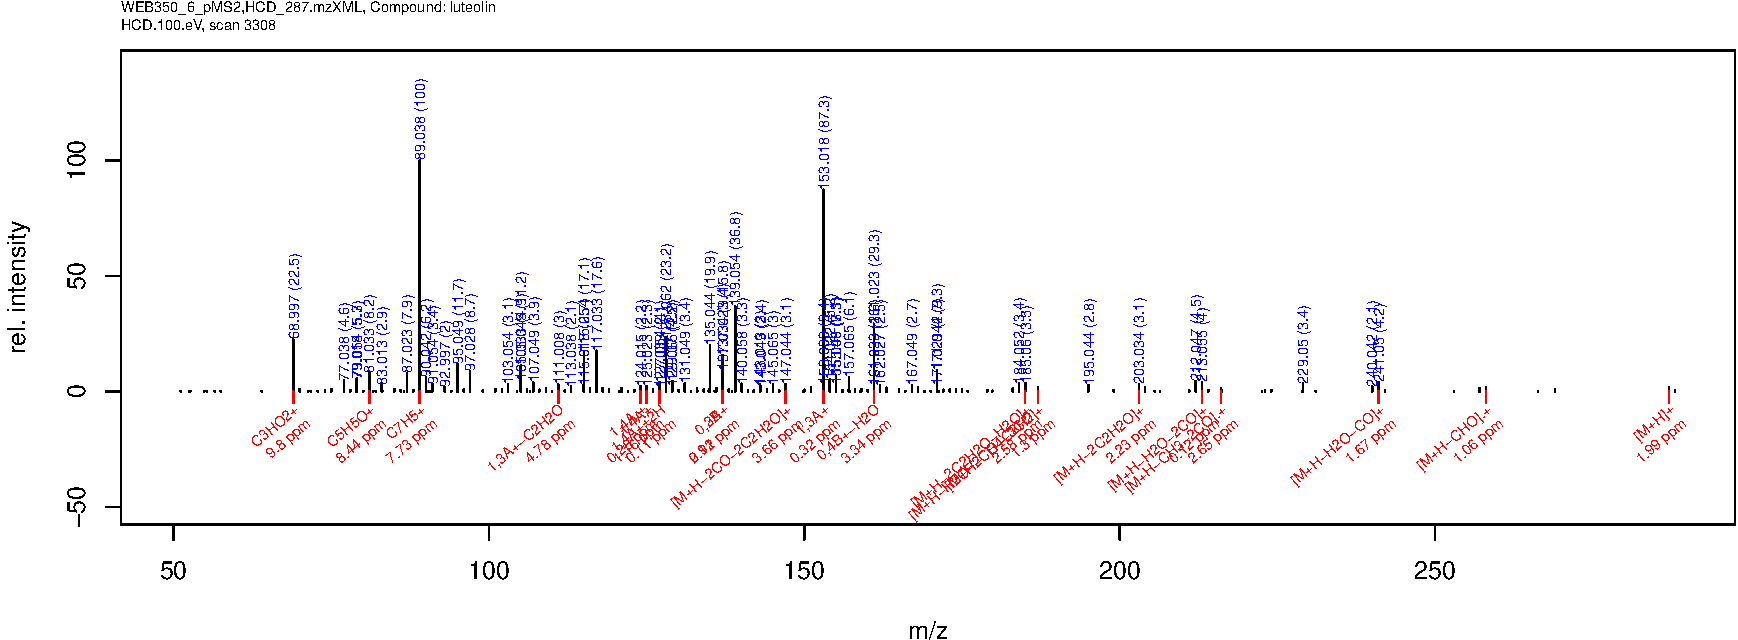
\includegraphics[width=\textwidth]{WEB350_files/figure-latex/unnamed-chunk-3-18}

\begin{table}[ht]
\centering
\begin{tabular}{rrrrl}
  \toprule
 & mz & int & ppm & fragment \\ 
  \midrule
1 & 69.00 & 22.5 & 1.32 & 1,3A+-2CO-C2H4 \\ 
  2 & 81.03 & 8.2 & 8.44 & C5H5O+ \\ 
  3 & 89.04 & 100.0 & 7.73 & C7H5+ \\ 
  4 & 97.03 & 8.7 & 0.83 & 1,3A+-2CO \\ 
  5 & 111.01 & 3.0 & 4.78 & 1,3A+-C2H2O \\ 
  6 & 124.02 & 2.2 & 0.28 & 1,4A.+ \\ 
  7 & 125.02 & 2.3 & 1.16 & 1,3A+-CO \\ 
  8 & 125.02 & 2.3 & 1.16 & 1,4A+ \\ 
  9 & 127.04 & 2.1 & 0.11 & 1,4A++2H \\ 
  10 & 137.02 & 15.8 & 2.92 & 0,2B+ \\ 
  11 & 137.02 & 15.8 & 0.11 & 0,3A+ \\ 
  12 & 147.04 & 3.1 & 3.66 & [M+H-2CO-2C2H2O]+ \\ 
  13 & 153.02 & 87.3 & 0.32 & 1,3A+ \\ 
  14 & 161.02 & 29.3 & 3.34 & 0,4B+-H2O \\ 
  15 & 185.02 & 1.9 & 2.58 & [M+H-2C2H2O-H2O]+ \\ 
  16 & 187.04 & 1.6 & 1.30 & [M+H-CH4-3CO]+ \\ 
  17 & 187.04 & 1.6 & 1.30 & [M+H-H2O-2CO-C2H2]+ \\ 
  18 & 203.03 & 3.1 & 2.23 & [M+H-2C2H2O]+ \\ 
  19 & 213.06 & 4.0 & 0.12 & [M+H-H2O-2CO]+ \\ 
  20 & 216.04 & 1.2 & 2.65 & [M+H-CH3-2CO].+ \\ 
  21 & 241.05 & 4.2 & 1.67 & [M+H-H2O-CO]+ \\ 
  22 & 258.05 & 1.7 & 1.06 & [M+H-CHO].+ \\ 
  23 & 287.05 & 1.6 & 1.99 & [M+H]+ \\ 
   \bottomrule
\end{tabular}
\end{table}

\clearpage\subsection{diosmetin.CID.45eV}
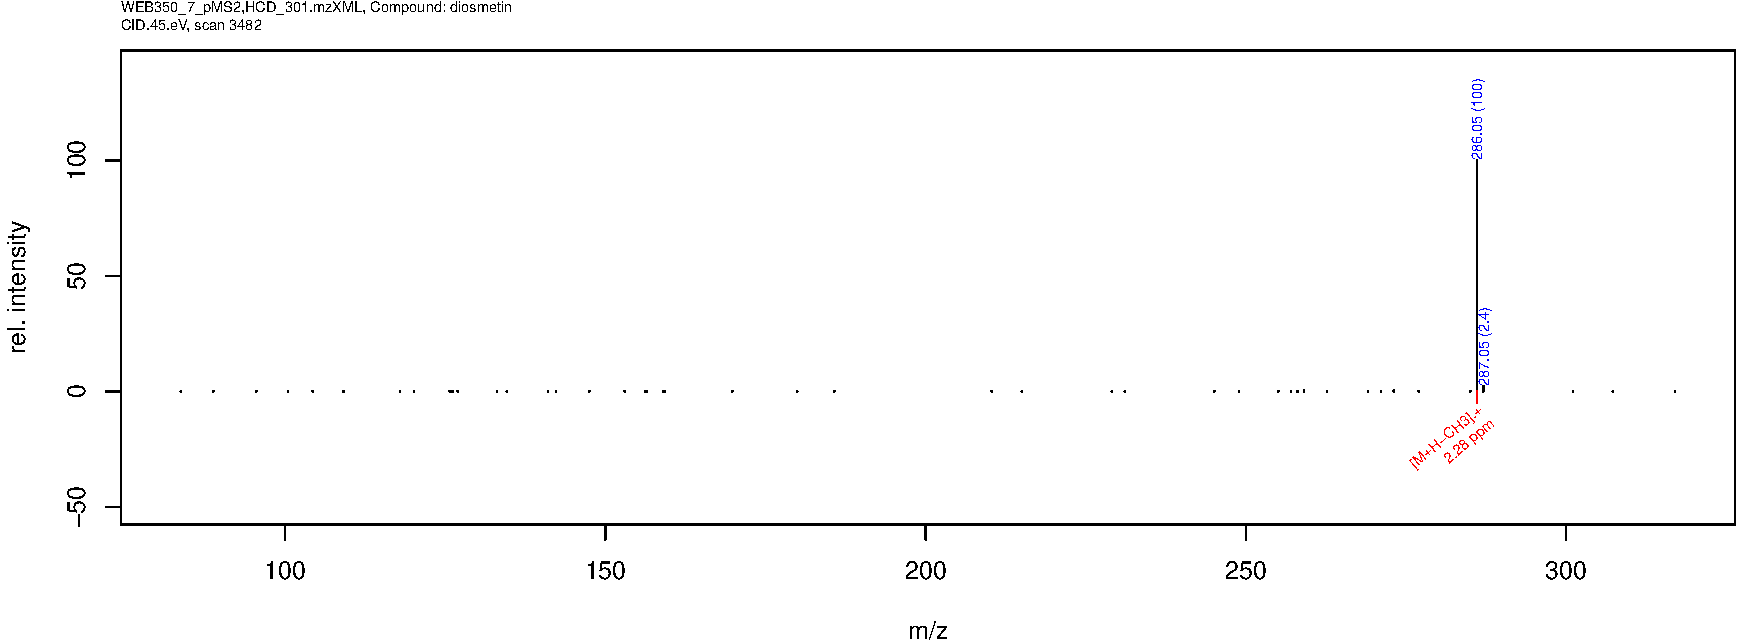
\includegraphics[width=\textwidth]{WEB350_files/figure-latex/unnamed-chunk-3-19}

\begin{table}[ht]
\centering
\begin{tabular}{rrrrl}
  \toprule
 & mz & int & ppm & fragment \\ 
  \midrule
1 & 286.05 & 100.0 & 2.28 & [M+H-CH3].+ \\ 
   \bottomrule
\end{tabular}
\end{table}

\clearpage\subsection{diosmetin.HCD.75eV}
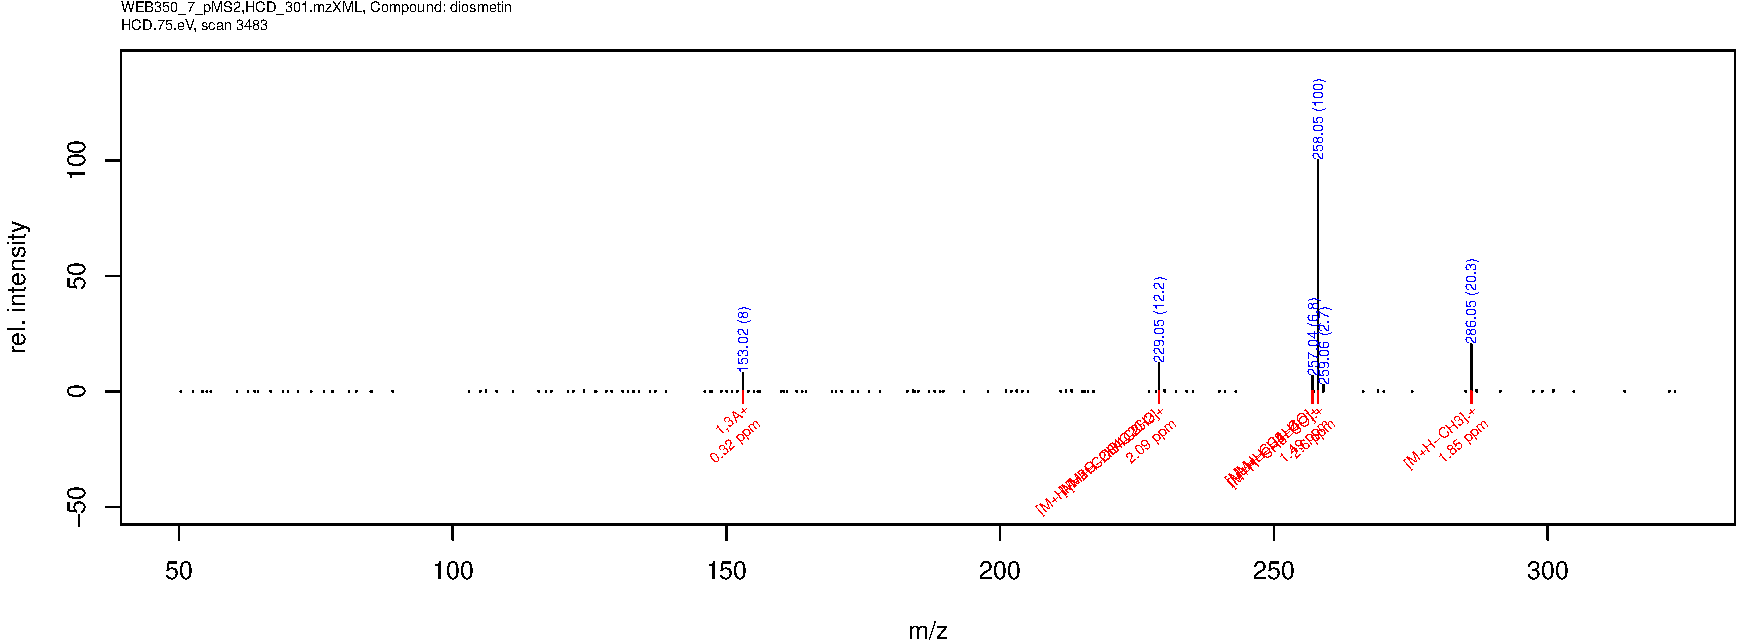
\includegraphics[width=\textwidth]{WEB350_files/figure-latex/unnamed-chunk-3-20}

\begin{table}[ht]
\centering
\begin{tabular}{rrrrl}
  \toprule
 & mz & int & ppm & fragment \\ 
  \midrule
1 & 153.02 & 8.0 & 0.32 & 1,3A+ \\ 
  2 & 229.05 & 12.2 & 2.09 & [M+H-CH4-2CO]+ \\ 
  3 & 229.05 & 12.2 & 2.09 & [M+H-H2O-CO-C2H2]+ \\ 
  4 & 257.04 & 6.8 & 1.49 & [M+H-CH4-CO]+ \\ 
  5 & 258.05 & 100.0 & 2.60 & [M+H-CH3-CO].+ \\ 
  6 & 286.05 & 20.3 & 1.85 & [M+H-CH3].+ \\ 
   \bottomrule
\end{tabular}
\end{table}

\clearpage\subsection{diosmetin.HCD.100eV}
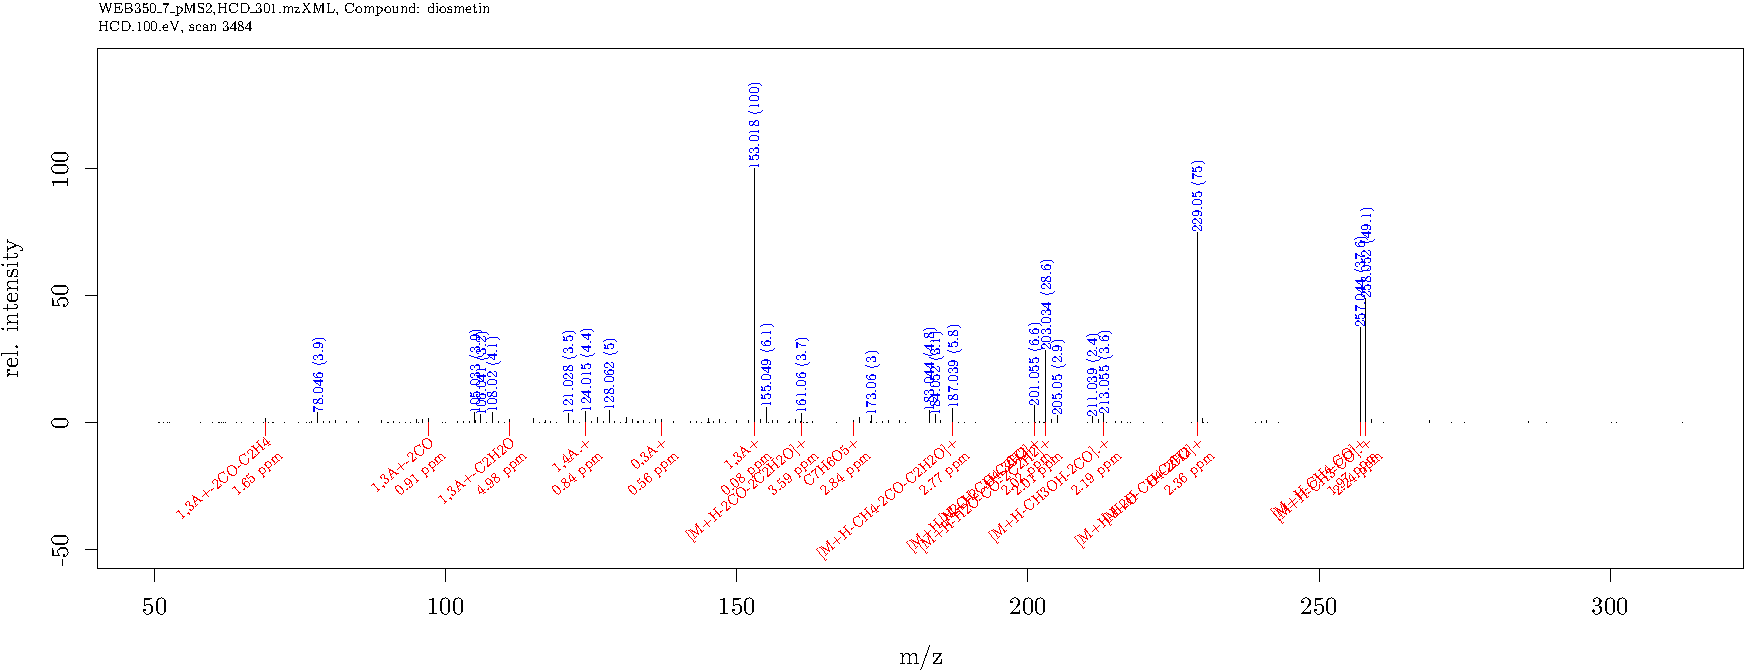
\includegraphics[width=\textwidth]{WEB350_files/figure-latex/unnamed-chunk-3-21}

\begin{table}[ht]
\centering
\begin{tabular}{rrrrl}
  \toprule
 & mz & int & ppm & fragment \\ 
  \midrule
1 & 69.00 & 1.8 & 1.65 & 1,3A+-2CO-C2H4 \\ 
  2 & 97.03 & 1.7 & 0.91 & 1,3A+-2CO \\ 
  3 & 111.01 & 1.3 & 4.98 & 1,3A+-C2H2O \\ 
  4 & 124.02 & 4.4 & 0.84 & 1,4A.+ \\ 
  5 & 137.02 & 1.5 & 0.56 & 0,3A+ \\ 
  6 & 153.02 & 100.0 & 0.08 & 1,3A+ \\ 
  7 & 161.06 & 3.7 & 3.59 & [M+H-2CO-2C2H2O]+ \\ 
  8 & 170.02 & 1.1 & 2.84 & C7H6O5+ \\ 
  9 & 173.06 & 3.0 & 2.46 & [M+H-CH4-4CO]+ \\ 
  10 & 187.04 & 5.8 & 2.77 & [M+H-CH4-2CO-C2H2O]+ \\ 
  11 & 201.05 & 6.6 & 2.02 & [M+H-CH4-3CO]+ \\ 
  12 & 201.05 & 6.6 & 2.02 & [M+H-H2O-2CO-C2H2]+ \\ 
  13 & 203.03 & 28.6 & 2.01 & [M+H-H2O-CO-2C2H2]+ \\ 
  14 & 213.05 & 3.6 & 2.19 & [M+H-CH3OH-2CO].+ \\ 
  15 & 229.05 & 75.0 & 2.36 & [M+H-CH4-2CO]+ \\ 
  16 & 229.05 & 75.0 & 2.36 & [M+H-H2O-CO-C2H2]+ \\ 
  17 & 257.04 & 37.6 & 1.97 & [M+H-CH4-CO]+ \\ 
  18 & 258.05 & 49.1 & 2.24 & [M+H-CH3-CO].+ \\ 
   \bottomrule
\end{tabular}
\end{table}

\clearpage\subsection{chrysoeriol.CID.45eV}
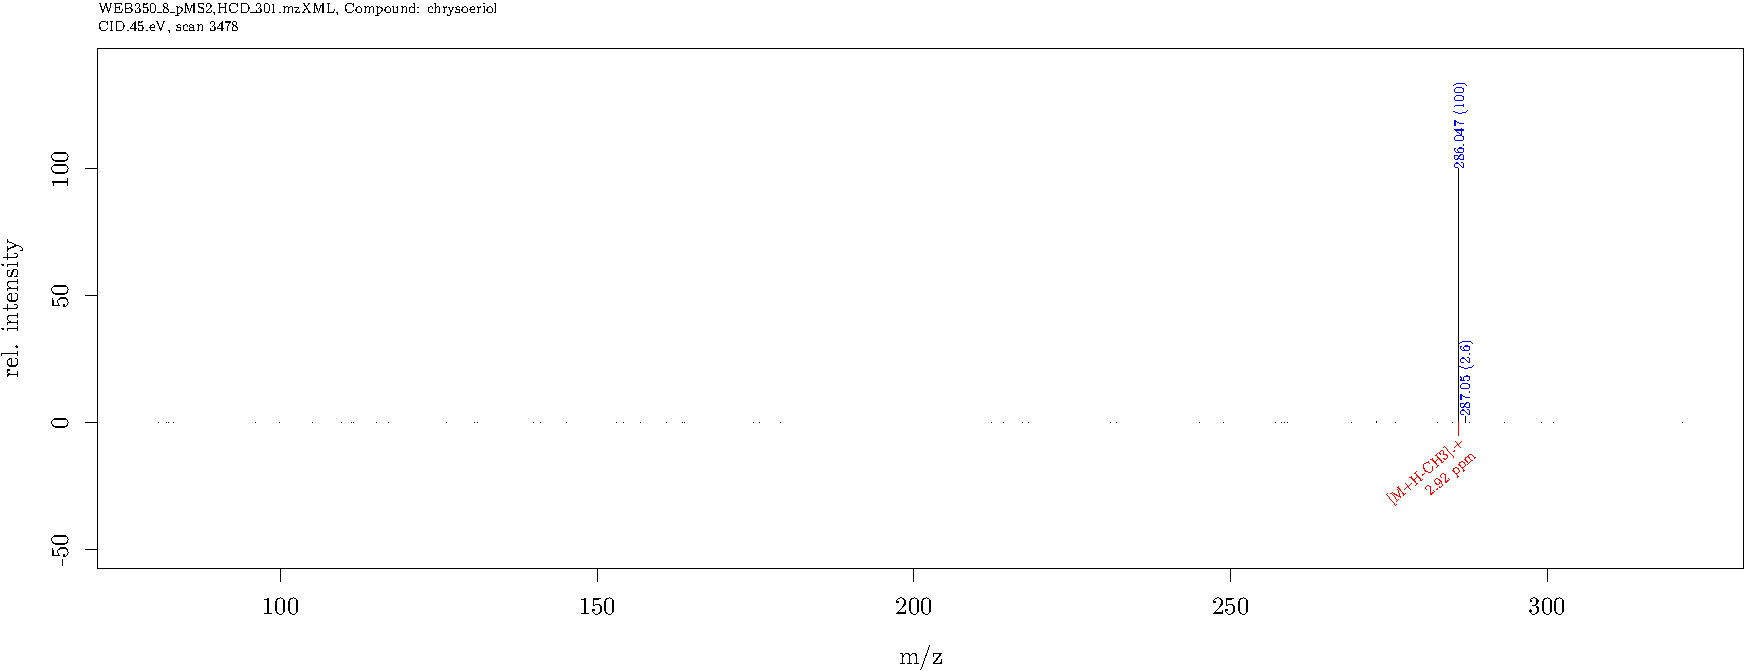
\includegraphics[width=\textwidth]{WEB350_files/figure-latex/unnamed-chunk-3-22}

\begin{table}[ht]
\centering
\begin{tabular}{rrrrl}
  \toprule
 & mz & int & ppm & fragment \\ 
  \midrule
1 & 286.05 & 100.0 & 2.92 & [M+H-CH3].+ \\ 
   \bottomrule
\end{tabular}
\end{table}

\clearpage\subsection{chrysoeriol.HCD.75eV}
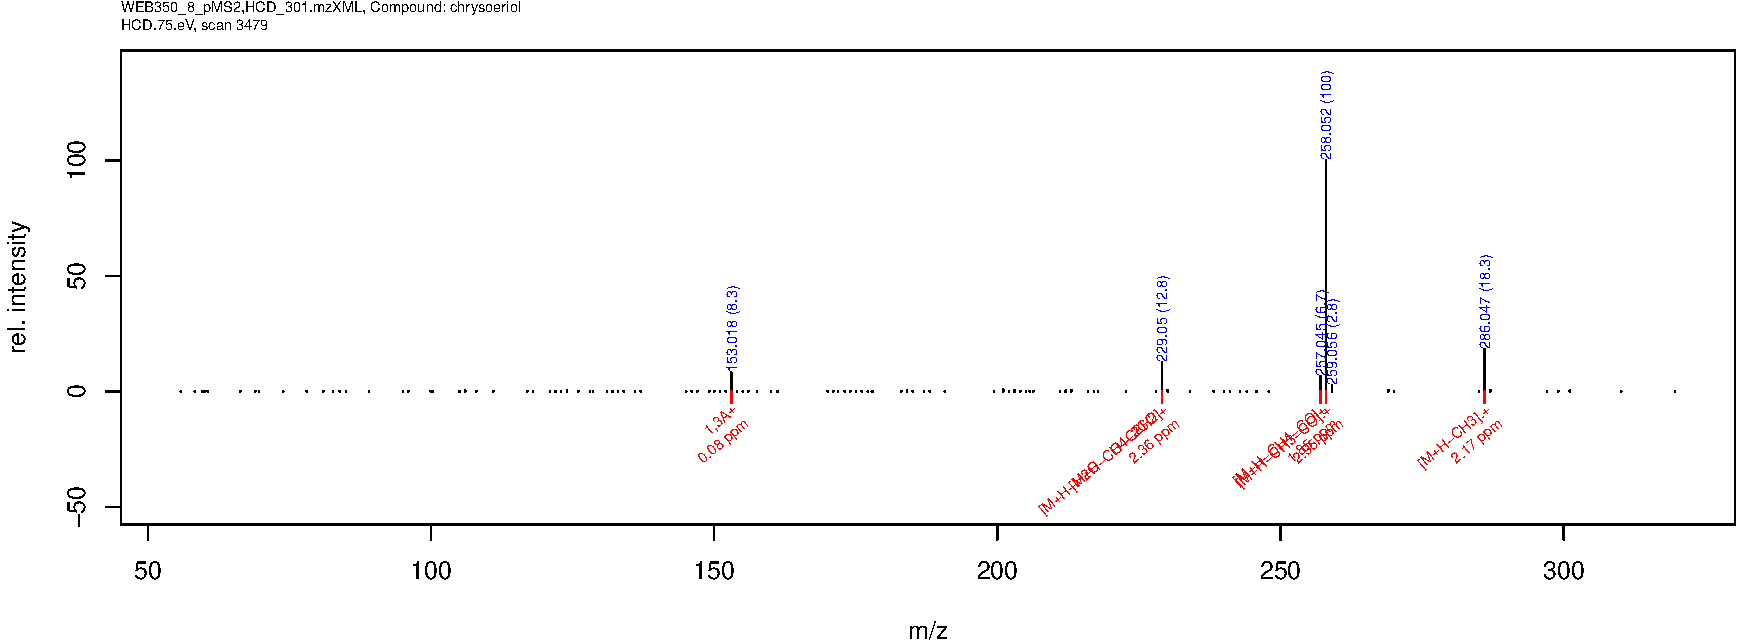
\includegraphics[width=\textwidth]{WEB350_files/figure-latex/unnamed-chunk-3-23}

\begin{table}[ht]
\centering
\begin{tabular}{rrrrl}
  \toprule
 & mz & int & ppm & fragment \\ 
  \midrule
1 & 153.02 & 8.3 & 0.08 & 1,3A+ \\ 
  2 & 229.05 & 12.8 & 2.36 & [M+H-CH4-2CO]+ \\ 
  3 & 229.05 & 12.8 & 2.36 & [M+H-H2O-CO-C2H2]+ \\ 
  4 & 257.04 & 6.7 & 1.85 & [M+H-CH4-CO]+ \\ 
  5 & 258.05 & 100.0 & 2.95 & [M+H-CH3-CO].+ \\ 
  6 & 286.05 & 18.3 & 2.17 & [M+H-CH3].+ \\ 
   \bottomrule
\end{tabular}
\end{table}

\clearpage\subsection{chrysoeriol.HCD.100eV}
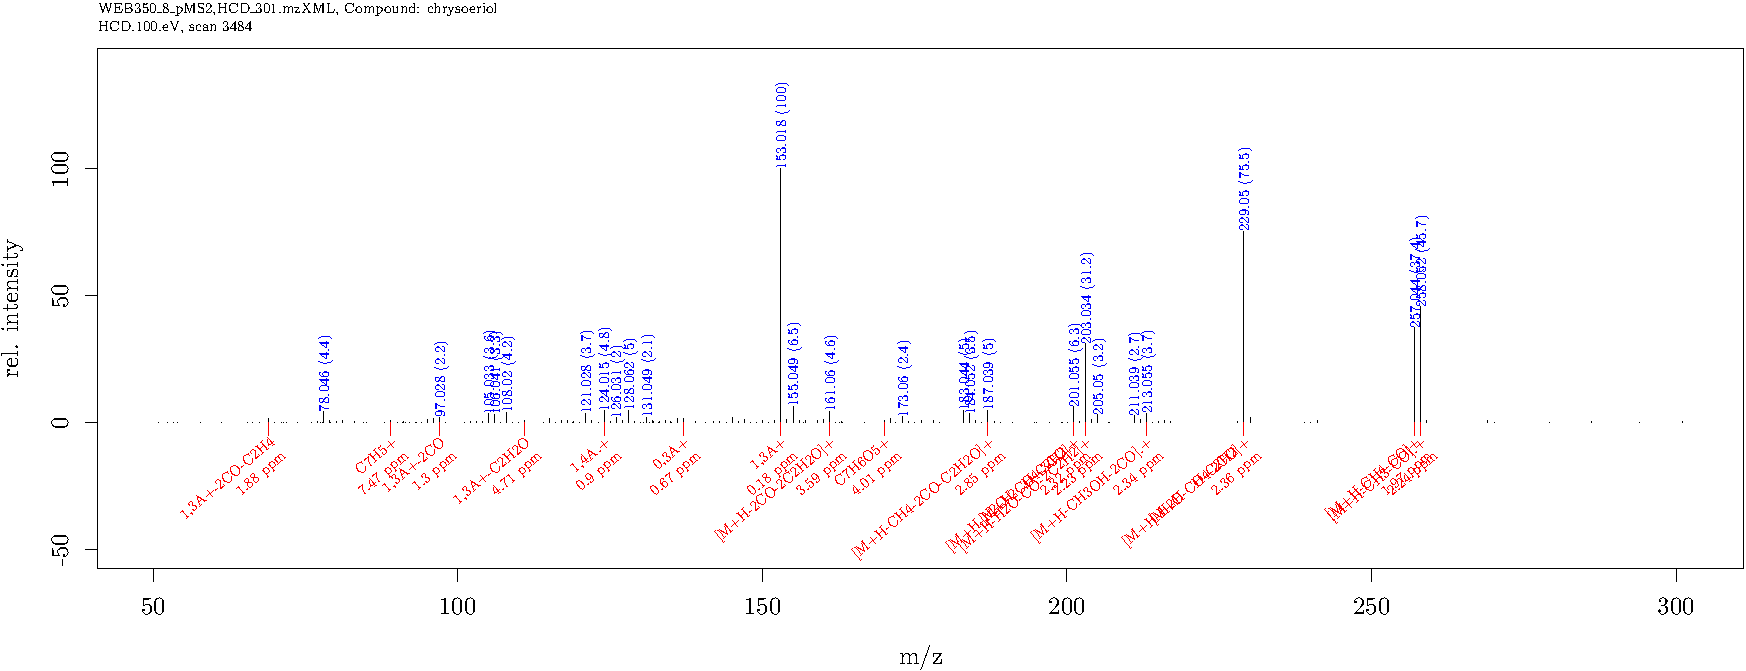
\includegraphics[width=\textwidth]{WEB350_files/figure-latex/unnamed-chunk-3-24}

\begin{table}[ht]
\centering
\begin{tabular}{rrrrl}
  \toprule
 & mz & int & ppm & fragment \\ 
  \midrule
1 & 69.00 & 1.9 & 1.88 & 1,3A+-2CO-C2H4 \\ 
  2 & 89.04 & 1.0 & 7.47 & C7H5+ \\ 
  3 & 97.03 & 2.2 & 1.30 & 1,3A+-2CO \\ 
  4 & 111.01 & 1.1 & 4.71 & 1,3A+-C2H2O \\ 
  5 & 124.02 & 4.8 & 0.90 & 1,4A.+ \\ 
  6 & 137.02 & 1.6 & 0.67 & 0,3A+ \\ 
  7 & 153.02 & 100.0 & 0.18 & 1,3A+ \\ 
  8 & 161.06 & 4.6 & 3.59 & [M+H-2CO-2C2H2O]+ \\ 
  9 & 170.02 & 1.1 & 4.01 & C7H6O5+ \\ 
  10 & 173.06 & 2.4 & 3.07 & [M+H-CH4-4CO]+ \\ 
  11 & 187.04 & 5.0 & 2.85 & [M+H-CH4-2CO-C2H2O]+ \\ 
  12 & 201.05 & 6.3 & 2.32 & [M+H-CH4-3CO]+ \\ 
  13 & 201.05 & 6.3 & 2.32 & [M+H-H2O-2CO-C2H2]+ \\ 
  14 & 203.03 & 31.2 & 2.23 & [M+H-H2O-CO-2C2H2]+ \\ 
  15 & 213.05 & 3.7 & 2.34 & [M+H-CH3OH-2CO].+ \\ 
  16 & 229.05 & 75.5 & 2.36 & [M+H-CH4-2CO]+ \\ 
  17 & 229.05 & 75.5 & 2.36 & [M+H-H2O-CO-C2H2]+ \\ 
  18 & 257.04 & 37.4 & 1.97 & [M+H-CH4-CO]+ \\ 
  19 & 258.05 & 45.7 & 2.24 & [M+H-CH3-CO].+ \\ 
   \bottomrule
\end{tabular}
\end{table}

\clearpage\subsection{kaempferol.CID.45eV}
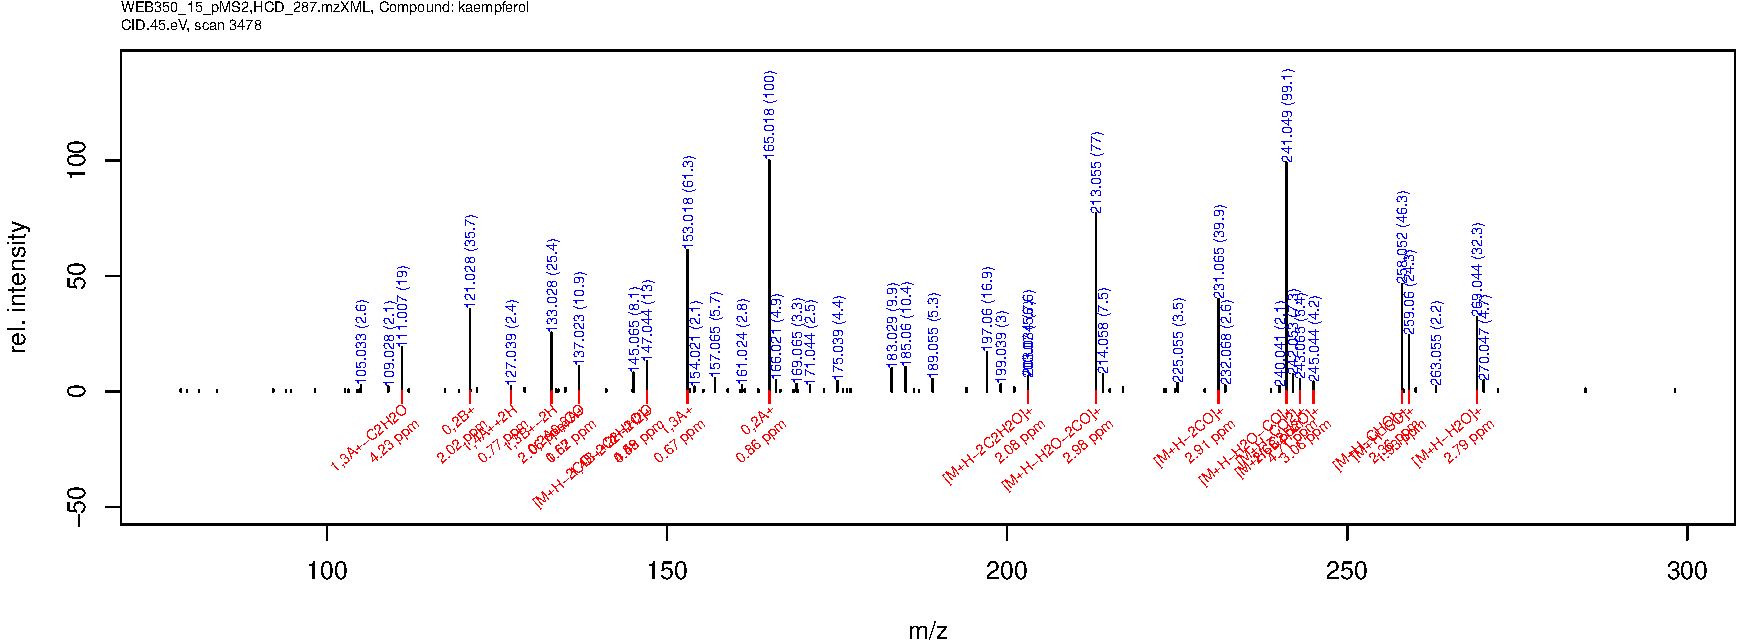
\includegraphics[width=\textwidth]{WEB350_files/figure-latex/unnamed-chunk-3-25}

\begin{table}[ht]
\centering
\begin{tabular}{rrrrl}
  \toprule
 & mz & int & ppm & fragment \\ 
  \midrule
1 & 111.01 & 19.0 & 4.23 & 1,3A+-C2H2O \\ 
  2 & 121.03 & 35.7 & 2.02 & 0,2B+ \\ 
  3 & 127.04 & 2.4 & 0.77 & 1,4A++2H \\ 
  4 & 133.03 & 25.4 & 2.06 & 1,3B+-2H \\ 
  5 & 137.02 & 10.9 & 1.52 & 0,2A+-CO \\ 
  6 & 137.02 & 10.9 & 0.67 & 0,3A+ \\ 
  7 & 147.04 & 13.0 & 0.48 & 1,4B++2H-H2O \\ 
  8 & 147.04 & 13.0 & 4.59 & [M+H-2CO-2C2H2O]+ \\ 
  9 & 153.02 & 61.3 & 0.67 & 1,3A+ \\ 
  10 & 165.02 & 100.0 & 0.86 & 0,2A+ \\ 
  11 & 199.04 & 3.0 & 4.45 & [M+H-CH3OH-2CO].+ \\ 
  12 & 203.03 & 6.6 & 2.08 & [M+H-2C2H2O]+ \\ 
  13 & 213.05 & 77.0 & 2.98 & [M+H-H2O-2CO]+ \\ 
  14 & 231.07 & 39.9 & 2.91 & [M+H-2CO]+ \\ 
  15 & 241.05 & 99.1 & 2.68 & [M+H-H2O-CO]+ \\ 
  16 & 243.06 & 5.4 & 4.71 & [M+H-CO2]+ \\ 
  17 & 245.04 & 4.2 & 3.06 & [M+H-C2H2O]+ \\ 
  18 & 258.05 & 46.3 & 2.36 & [M+H-CHO].+ \\ 
  19 & 259.06 & 24.3 & 1.93 & [M+H-CO]+ \\ 
  20 & 269.04 & 32.3 & 2.79 & [M+H-H2O]+ \\ 
   \bottomrule
\end{tabular}
\end{table}

\clearpage\subsection{kaempferol.HCD.75eV}
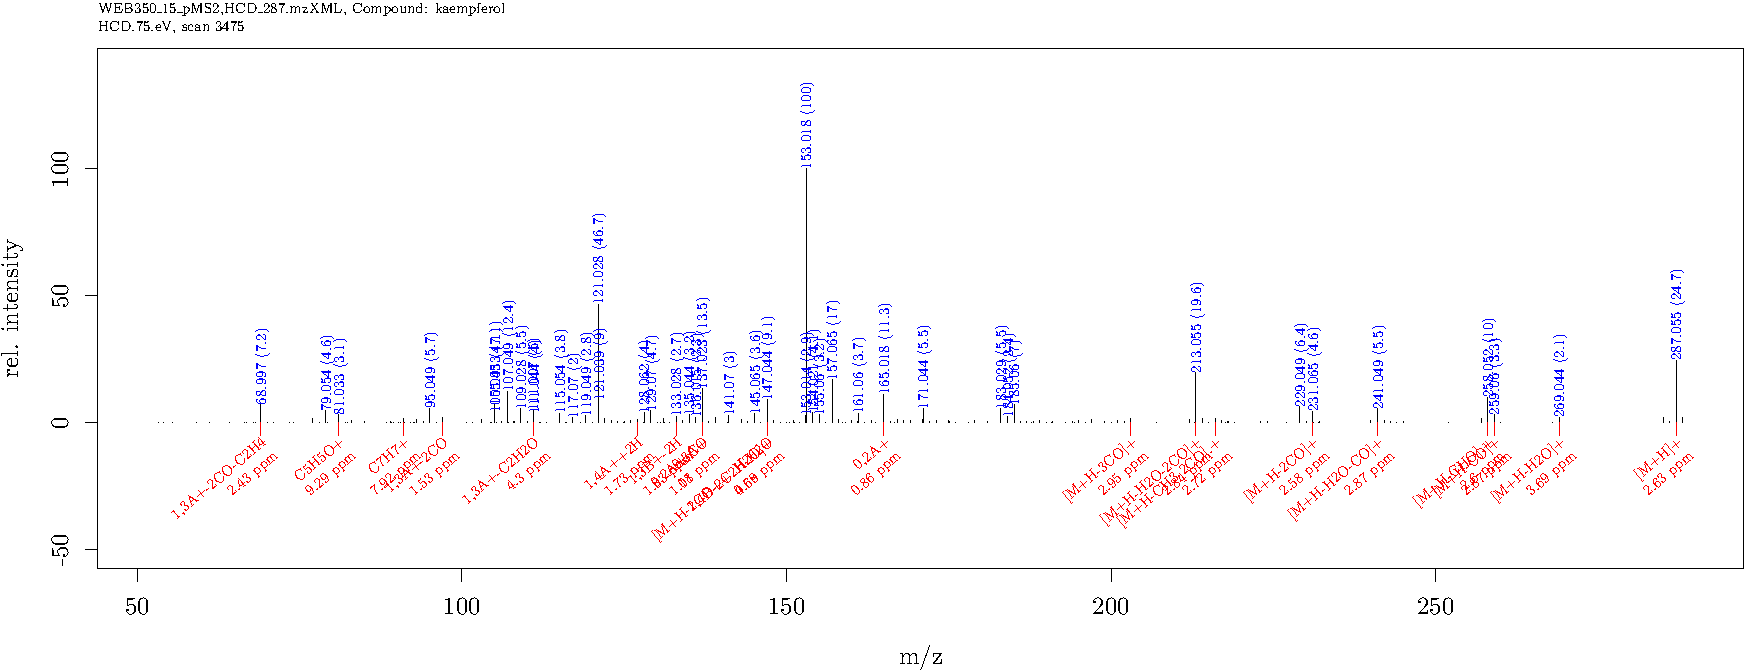
\includegraphics[width=\textwidth]{WEB350_files/figure-latex/unnamed-chunk-3-26}

\begin{table}[ht]
\centering
\begin{tabular}{rrrrl}
  \toprule
 & mz & int & ppm & fragment \\ 
  \midrule
1 & 69.00 & 7.2 & 2.43 & 1,3A+-2CO-C2H4 \\ 
  2 & 81.03 & 3.1 & 9.29 & C5H5O+ \\ 
  3 & 91.05 & 1.9 & 7.92 & C7H7+ \\ 
  4 & 97.03 & 1.9 & 1.53 & 1,3A+-2CO \\ 
  5 & 111.01 & 5.0 & 4.30 & 1,3A+-C2H2O \\ 
  6 & 127.04 & 1.4 & 1.73 & 1,4A++2H \\ 
  7 & 133.03 & 2.7 & 1.83 & 1,3B+-2H \\ 
  8 & 137.02 & 13.5 & 1.08 & 0,2A+-CO \\ 
  9 & 137.02 & 13.5 & 1.11 & 0,3A+ \\ 
  10 & 147.04 & 9.1 & 0.58 & 1,4B++2H-H2O \\ 
  11 & 147.04 & 9.1 & 4.69 & [M+H-2CO-2C2H2O]+ \\ 
  12 & 165.02 & 11.3 & 0.86 & 0,2A+ \\ 
  13 & 203.07 & 1.5 & 2.95 & [M+H-3CO]+ \\ 
  14 & 213.05 & 19.6 & 2.84 & [M+H-H2O-2CO]+ \\ 
  15 & 216.04 & 1.8 & 2.72 & [M+H-CH3-2CO].+ \\ 
  16 & 231.07 & 4.6 & 2.58 & [M+H-2CO]+ \\ 
  17 & 241.05 & 5.5 & 2.87 & [M+H-H2O-CO]+ \\ 
  18 & 258.05 & 10.0 & 2.60 & [M+H-CHO].+ \\ 
  19 & 259.06 & 3.3 & 2.87 & [M+H-CO]+ \\ 
  20 & 269.04 & 2.1 & 3.69 & [M+H-H2O]+ \\ 
  21 & 287.05 & 24.7 & 2.63 & [M+H]+ \\ 
   \bottomrule
\end{tabular}
\end{table}

\clearpage\subsection{kaempferol.HCD.100eV}
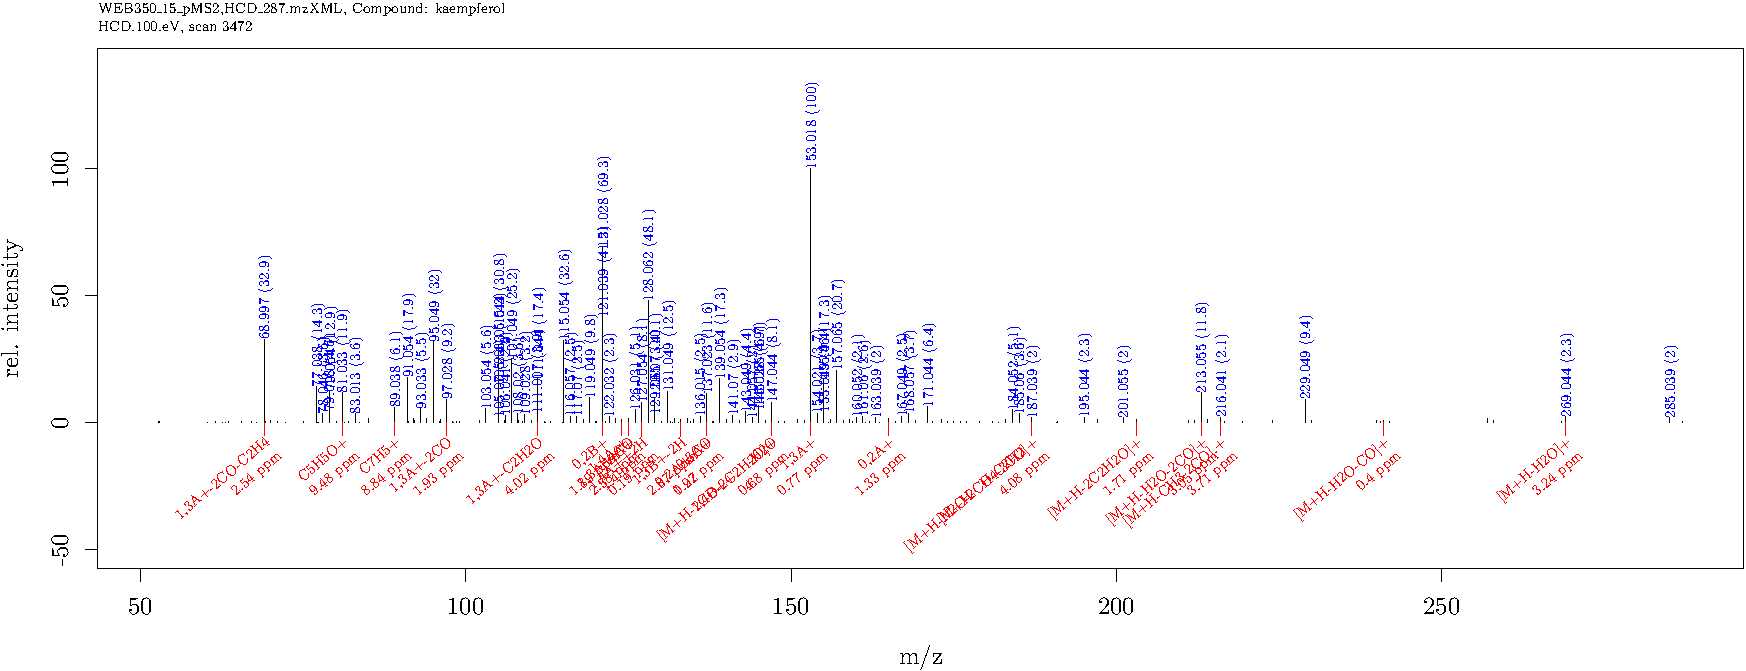
\includegraphics[width=\textwidth]{WEB350_files/figure-latex/unnamed-chunk-3-27}

\begin{table}[ht]
\centering
\begin{tabular}{rrrrl}
  \toprule
 & mz & int & ppm & fragment \\ 
  \midrule
1 & 69.00 & 32.9 & 2.54 & 1,3A+-2CO-C2H4 \\ 
  2 & 81.03 & 11.9 & 9.48 & C5H5O+ \\ 
  3 & 89.04 & 6.1 & 8.84 & C7H5+ \\ 
  4 & 97.03 & 9.2 & 1.93 & 1,3A+-2CO \\ 
  5 & 111.01 & 3.9 & 4.02 & 1,3A+-C2H2O \\ 
  6 & 121.03 & 69.3 & 1.89 & 0,2B+ \\ 
  7 & 124.02 & 1.3 & 2.38 & 1,4A.+ \\ 
  8 & 125.02 & 1.6 & 1.40 & 1,3A+-CO \\ 
  9 & 125.02 & 1.6 & 1.40 & 1,4A+ \\ 
  10 & 127.04 & 1.6 & 0.19 & 1,4A++2H \\ 
  11 & 133.03 & 1.2 & 2.87 & 1,3B+-2H \\ 
  12 & 137.02 & 11.6 & 0.97 & 0,2A+-CO \\ 
  13 & 137.02 & 11.6 & 1.22 & 0,3A+ \\ 
  14 & 147.04 & 8.1 & 0.68 & 1,4B++2H-H2O \\ 
  15 & 147.04 & 8.1 & 4.80 & [M+H-2CO-2C2H2O]+ \\ 
  16 & 153.02 & 100.0 & 0.77 & 1,3A+ \\ 
  17 & 159.04 & 1.3 & 2.80 & [M+H-CH4-4CO]+ \\ 
  18 & 165.02 & 1.9 & 1.33 & 0,2A+ \\ 
  19 & 187.04 & 2.0 & 4.08 & [M+H-CH4-3CO]+ \\ 
  20 & 187.04 & 2.0 & 4.08 & [M+H-H2O-2CO-C2H2]+ \\ 
  21 & 203.03 & 1.3 & 1.71 & [M+H-2C2H2O]+ \\ 
  22 & 213.05 & 11.8 & 3.05 & [M+H-H2O-2CO]+ \\ 
  23 & 216.04 & 2.1 & 3.71 & [M+H-CH3-2CO].+ \\ 
  24 & 241.05 & 1.0 & 0.40 & [M+H-H2O-CO]+ \\ 
  25 & 269.04 & 2.3 & 3.24 & [M+H-H2O]+ \\ 
   \bottomrule
\end{tabular}
\end{table}

\clearpage\subsection{quercetin.CID.45eV}
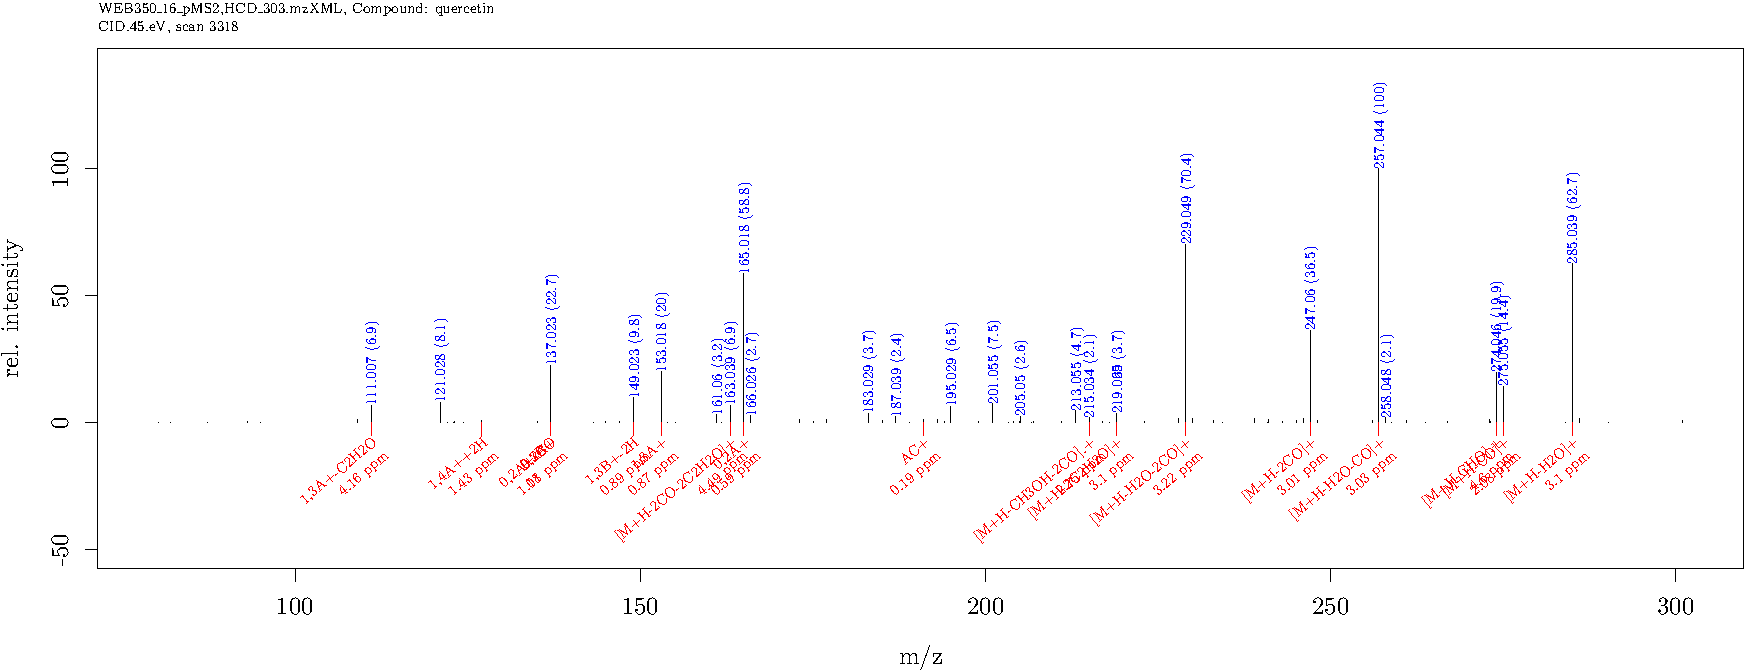
\includegraphics[width=\textwidth]{WEB350_files/figure-latex/unnamed-chunk-3-28}

\begin{table}[ht]
\centering
\begin{tabular}{rrrrl}
  \toprule
 & mz & int & ppm & fragment \\ 
  \midrule
1 & 111.01 & 6.9 & 4.16 & 1,3A+-C2H2O \\ 
  2 & 127.04 & 1.0 & 1.43 & 1,4A++2H \\ 
  3 & 137.02 & 22.7 & 1.08 & 0,2A+-CO \\ 
  4 & 137.02 & 22.7 & 1.08 & 0,2B+ \\ 
  5 & 137.02 & 22.7 & 1.11 & 0,3A+ \\ 
  6 & 149.02 & 9.8 & 0.89 & 1,3B+-2H \\ 
  7 & 153.02 & 20.0 & 0.87 & 1,3A+ \\ 
  8 & 163.04 & 6.9 & 4.49 & [M+H-2CO-2C2H2O]+ \\ 
  9 & 165.02 & 58.8 & 0.59 & 0,2A+ \\ 
  10 & 191.03 & 1.2 & 0.19 & AC+ \\ 
  11 & 215.03 & 2.1 & 2.75 & [M+H-CH3OH-2CO].+ \\ 
  12 & 219.03 & 3.7 & 3.10 & [M+H-2C2H2O]+ \\ 
  13 & 229.05 & 70.4 & 3.22 & [M+H-H2O-2CO]+ \\ 
  14 & 247.06 & 36.5 & 3.01 & [M+H-2CO]+ \\ 
  15 & 257.04 & 100.0 & 3.03 & [M+H-H2O-CO]+ \\ 
  16 & 274.05 & 19.9 & 4.60 & [M+H-CHO].+ \\ 
  17 & 275.05 & 14.4 & 2.08 & [M+H-CO]+ \\ 
  18 & 285.04 & 62.7 & 3.10 & [M+H-H2O]+ \\ 
   \bottomrule
\end{tabular}
\end{table}

\clearpage\subsection{quercetin.HCD.75eV}
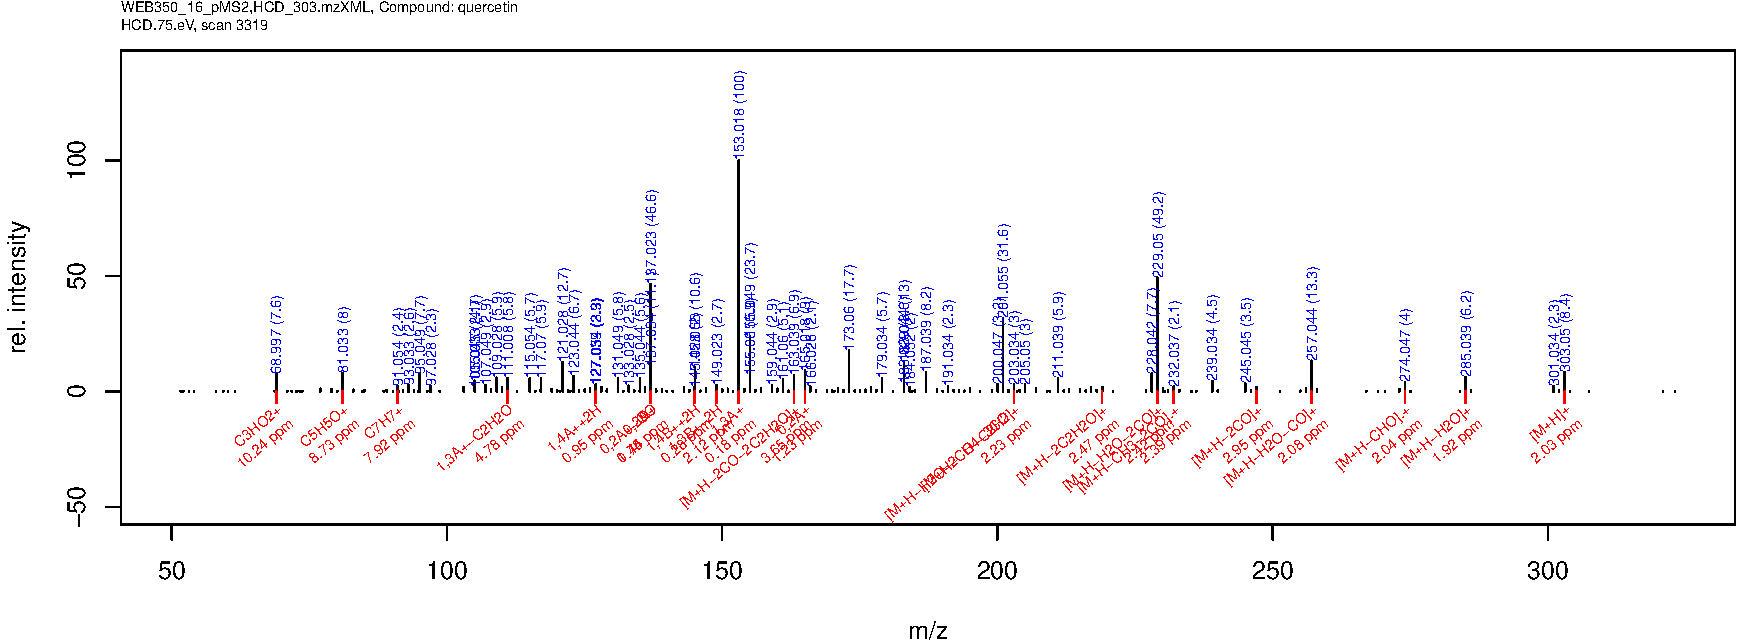
\includegraphics[width=\textwidth]{WEB350_files/figure-latex/unnamed-chunk-3-29}

\begin{table}[ht]
\centering
\begin{tabular}{rrrrl}
  \toprule
 & mz & int & ppm & fragment \\ 
  \midrule
1 & 69.00 & 7.6 & 1.76 & 1,3A+-2CO-C2H4 \\ 
  2 & 81.03 & 8.0 & 8.73 & C5H5O+ \\ 
  3 & 91.05 & 2.4 & 7.92 & C7H7+ \\ 
  4 & 97.03 & 2.3 & 1.14 & 1,3A+-2CO \\ 
  5 & 111.01 & 5.8 & 4.78 & 1,3A+-C2H2O \\ 
  6 & 127.04 & 2.9 & 0.95 & 1,4A++2H \\ 
  7 & 137.02 & 46.6 & 1.75 & 0,2A+-CO \\ 
  8 & 137.02 & 46.6 & 1.75 & 0,2B+ \\ 
  9 & 137.02 & 46.6 & 0.44 & 0,3A+ \\ 
  10 & 145.03 & 2.0 & 0.28 & 1,4B++2H \\ 
  11 & 149.02 & 2.7 & 2.12 & 1,3B+-2H \\ 
  12 & 153.02 & 100.0 & 0.18 & 1,3A+ \\ 
  13 & 163.04 & 6.9 & 3.65 & [M+H-2CO-2C2H2O]+ \\ 
  14 & 165.02 & 9.0 & 1.23 & 0,2A+ \\ 
  15 & 191.03 & 2.3 & 0.03 & AC+ \\ 
  16 & 203.03 & 3.0 & 2.23 & [M+H-CH4-3CO]+ \\ 
  17 & 203.03 & 3.0 & 2.23 & [M+H-H2O-2CO-C2H2]+ \\ 
  18 & 219.03 & 1.1 & 2.47 & [M+H-2C2H2O]+ \\ 
  19 & 229.05 & 49.2 & 2.42 & [M+H-H2O-2CO]+ \\ 
  20 & 232.04 & 2.1 & 2.39 & [M+H-CH3-2CO].+ \\ 
  21 & 247.06 & 1.9 & 2.95 & [M+H-2CO]+ \\ 
  22 & 257.04 & 13.3 & 2.08 & [M+H-H2O-CO]+ \\ 
  23 & 274.05 & 4.0 & 2.04 & [M+H-CHO].+ \\ 
  24 & 285.04 & 6.2 & 1.92 & [M+H-H2O]+ \\ 
  25 & 303.05 & 8.4 & 2.03 & [M+H]+ \\ 
   \bottomrule
\end{tabular}
\end{table}

\clearpage\subsection{quercetin.HCD.100eV}
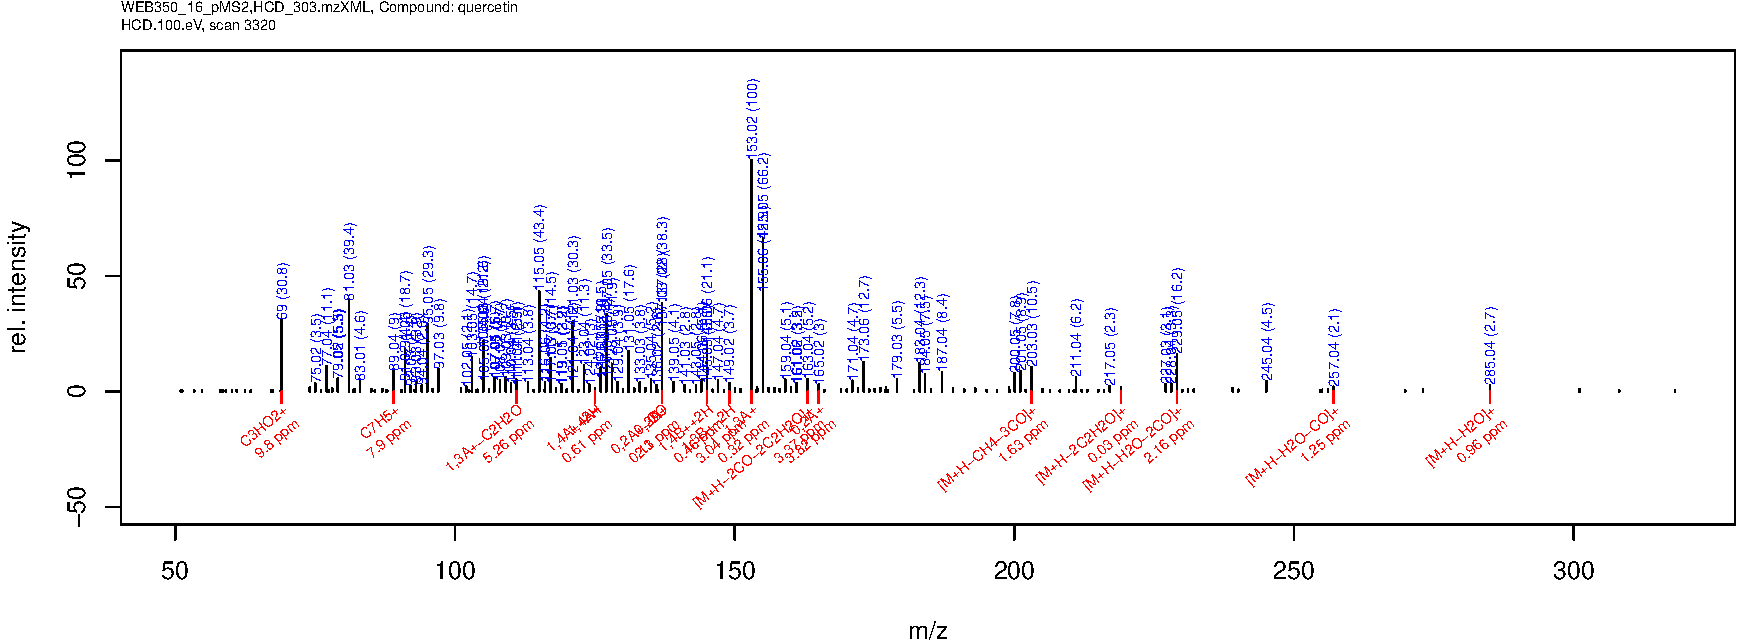
\includegraphics[width=\textwidth]{WEB350_files/figure-latex/unnamed-chunk-3-30}

\begin{table}[ht]
\centering
\begin{tabular}{rrrrl}
  \toprule
 & mz & int & ppm & fragment \\ 
  \midrule
1 & 69.00 & 30.8 & 1.32 & 1,3A+-2CO-C2H4 \\ 
  2 & 81.03 & 39.4 & 8.35 & C5H5O+ \\ 
  3 & 89.04 & 9.0 & 7.90 & C7H5+ \\ 
  4 & 97.03 & 9.8 & 1.14 & 1,3A+-2CO \\ 
  5 & 111.01 & 5.1 & 5.26 & 1,3A+-C2H2O \\ 
  6 & 124.02 & 3.0 & 0.47 & 1,4A.+ \\ 
  7 & 125.02 & 1.4 & 0.61 & 1,3A+-CO \\ 
  8 & 125.02 & 1.4 & 0.61 & 1,4A+ \\ 
  9 & 127.04 & 6.4 & 0.05 & 1,4A++2H \\ 
  10 & 137.02 & 38.3 & 2.30 & 0,2A+-CO \\ 
  11 & 137.02 & 38.3 & 2.30 & 0,2B+ \\ 
  12 & 137.02 & 38.3 & 0.11 & 0,3A+ \\ 
  13 & 145.03 & 3.6 & 0.46 & 1,4B++2H \\ 
  14 & 149.02 & 3.7 & 3.04 & 1,3B+-2H \\ 
  15 & 153.02 & 100.0 & 0.32 & 1,3A+ \\ 
  16 & 163.04 & 5.2 & 3.37 & [M+H-2CO-2C2H2O]+ \\ 
  17 & 165.02 & 3.0 & 3.82 & 0,2A+ \\ 
  18 & 175.04 & 1.2 & 1.04 & [M+H-CH4-4CO]+ \\ 
  19 & 203.03 & 10.5 & 1.63 & [M+H-CH4-3CO]+ \\ 
  20 & 203.03 & 10.5 & 1.63 & [M+H-H2O-2CO-C2H2]+ \\ 
  21 & 219.03 & 1.6 & 0.03 & [M+H-2C2H2O]+ \\ 
  22 & 229.05 & 16.2 & 2.16 & [M+H-H2O-2CO]+ \\ 
  23 & 257.04 & 2.1 & 1.25 & [M+H-H2O-CO]+ \\ 
  24 & 285.04 & 2.7 & 0.96 & [M+H-H2O]+ \\ 
   \bottomrule
\end{tabular}
\end{table}

\clearpage\subsection{myricetin.CID.45eV}
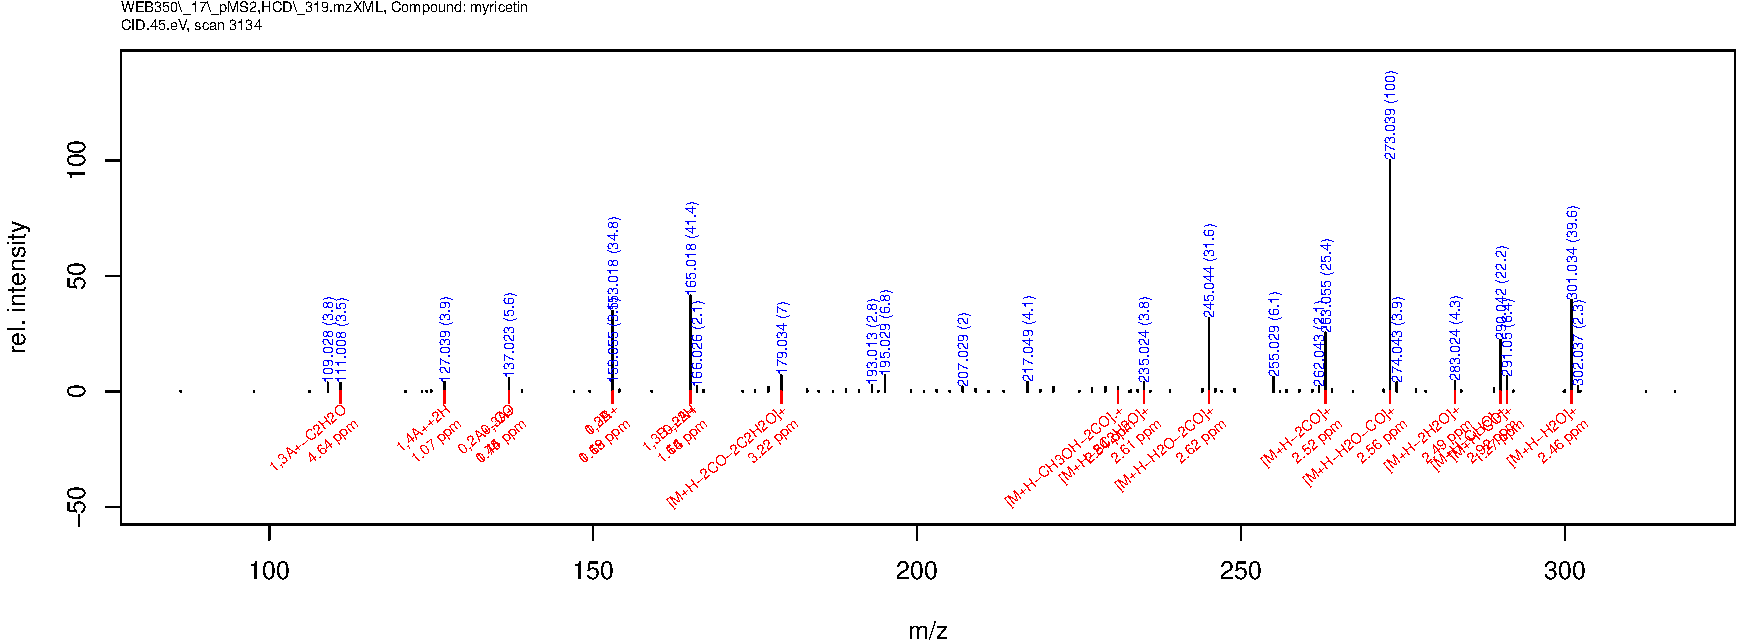
\includegraphics[width=\textwidth]{WEB350_files/figure-latex/unnamed-chunk-3-31}

\begin{table}[ht]
\centering
\begin{tabular}{rrrrl}
  \toprule
 & mz & int & ppm & fragment \\ 
  \midrule
1 & 111.01 & 3.5 & 4.64 & 1,3A+-C2H2O \\ 
  2 & 127.04 & 3.9 & 1.07 & 1,4A++2H \\ 
  3 & 137.02 & 5.6 & 1.75 & 0,2A+-CO \\ 
  4 & 137.02 & 5.6 & 0.44 & 0,3A+ \\ 
  5 & 153.02 & 34.8 & 1.69 & 0,2B+ \\ 
  6 & 153.02 & 34.8 & 0.18 & 1,3A+ \\ 
  7 & 165.02 & 41.4 & 1.14 & 0,2A+ \\ 
  8 & 165.02 & 41.4 & 1.66 & 1,3B+-2H \\ 
  9 & 179.03 & 7.0 & 3.22 & [M+H-2CO-2C2H2O]+ \\ 
  10 & 231.03 & 1.8 & 2.54 & [M+H-CH3OH-2CO].+ \\ 
  11 & 235.02 & 3.8 & 2.61 & [M+H-2C2H2O]+ \\ 
  12 & 245.04 & 31.6 & 2.62 & [M+H-H2O-2CO]+ \\ 
  13 & 263.05 & 25.4 & 2.52 & [M+H-2CO]+ \\ 
  14 & 273.04 & 100.0 & 2.56 & [M+H-H2O-CO]+ \\ 
  15 & 283.02 & 4.3 & 2.49 & [M+H-2H2O]+ \\ 
  16 & 290.04 & 22.2 & 2.92 & [M+H-CHO].+ \\ 
  17 & 291.05 & 6.4 & 1.27 & [M+H-CO]+ \\ 
  18 & 301.03 & 39.6 & 2.46 & [M+H-H2O]+ \\ 
   \bottomrule
\end{tabular}
\end{table}

\clearpage\subsection{myricetin.HCD.75eV}
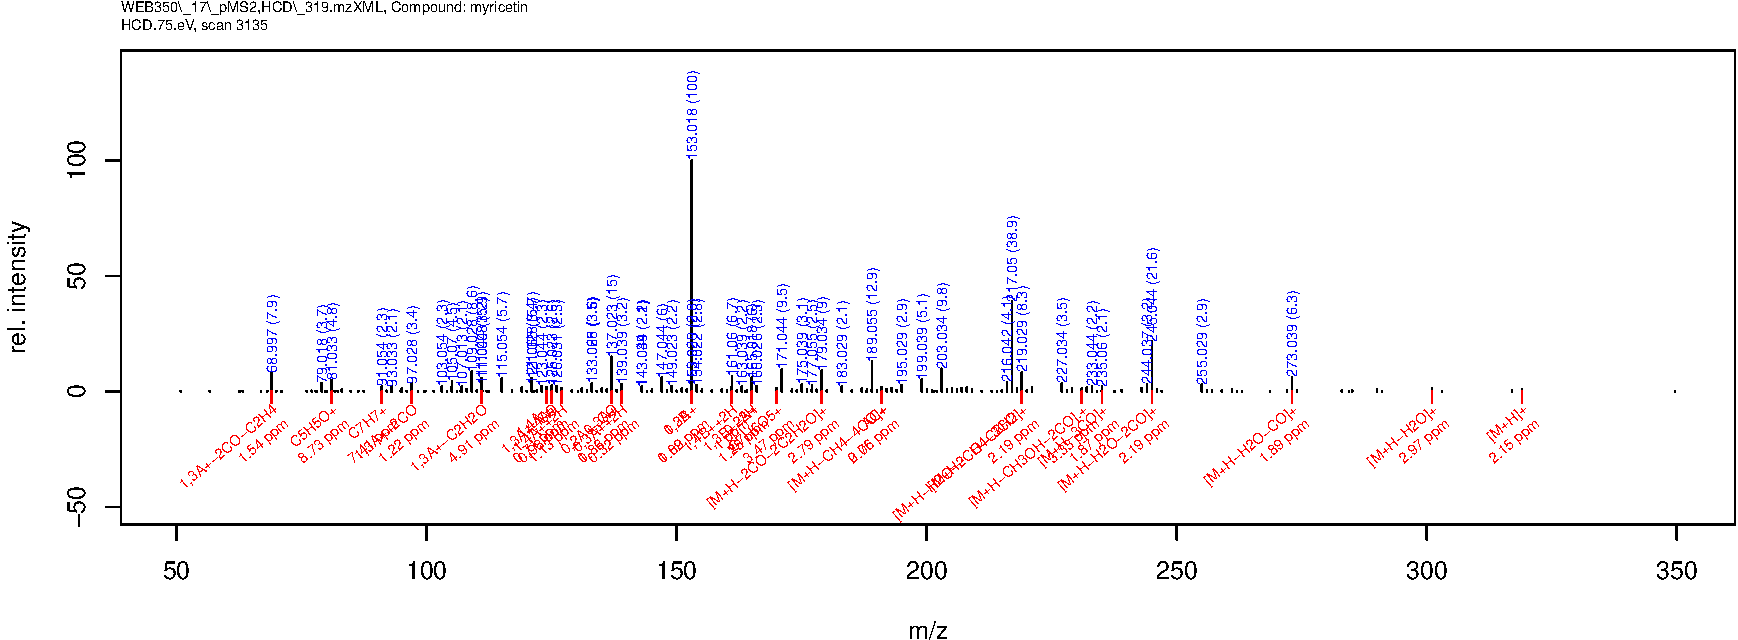
\includegraphics[width=\textwidth]{WEB350_files/figure-latex/unnamed-chunk-3-32}

\begin{table}[ht]
\centering
\begin{tabular}{rrrrl}
  \toprule
 & mz & int & ppm & fragment \\ 
  \midrule
1 & 69.00 & 7.9 & 1.54 & 1,3A+-2CO-C2H4 \\ 
  2 & 81.03 & 4.8 & 8.73 & C5H5O+ \\ 
  3 & 91.05 & 2.3 & 7.41 & C7H7+ \\ 
  4 & 97.03 & 3.4 & 1.22 & 1,3A+-2CO \\ 
  5 & 111.01 & 5.9 & 4.91 & 1,3A+-C2H2O \\ 
  6 & 124.02 & 2.0 & 0.71 & 1,4A.+ \\ 
  7 & 125.02 & 2.6 & 0.98 & 1,3A+-CO \\ 
  8 & 125.02 & 2.6 & 0.98 & 1,4A+ \\ 
  9 & 127.04 & 1.6 & 1.13 & 1,4A++2H \\ 
  10 & 137.02 & 15.0 & 1.86 & 0,2A+-CO \\ 
  11 & 137.02 & 15.0 & 0.33 & 0,3A+ \\ 
  12 & 139.04 & 3.2 & 0.32 & 0,3A++2H \\ 
  13 & 153.02 & 100.0 & 1.89 & 0,2B+ \\ 
  14 & 153.02 & 100.0 & 0.02 & 1,3A+ \\ 
  15 & 161.02 & 1.9 & 1.00 & 1,4B++2H \\ 
  16 & 165.02 & 6.0 & 1.23 & 0,2A+ \\ 
  17 & 165.02 & 6.0 & 1.75 & 1,3B+-2H \\ 
  18 & 170.02 & 1.4 & 3.47 & C7H6O5+ \\ 
  19 & 179.03 & 9.0 & 2.79 & [M+H-2CO-2C2H2O]+ \\ 
  20 & 191.03 & 1.9 & 0.75 & AC+ \\ 
  21 & 191.03 & 1.9 & 2.06 & [M+H-CH4-4CO]+ \\ 
  22 & 219.03 & 8.3 & 2.19 & [M+H-CH4-3CO]+ \\ 
  23 & 219.03 & 8.3 & 2.19 & [M+H-H2O-2CO-C2H2]+ \\ 
  24 & 231.03 & 1.4 & 3.33 & [M+H-CH3OH-2CO].+ \\ 
  25 & 235.06 & 2.1 & 1.87 & [M+H-3CO]+ \\ 
  26 & 245.04 & 21.6 & 2.19 & [M+H-H2O-2CO]+ \\ 
  27 & 273.04 & 6.3 & 1.89 & [M+H-H2O-CO]+ \\ 
  28 & 301.03 & 1.4 & 2.97 & [M+H-H2O]+ \\ 
  29 & 319.04 & 1.1 & 2.15 & [M+H]+ \\ 
   \bottomrule
\end{tabular}
\end{table}

\clearpage\subsection{myricetin.HCD.100eV}
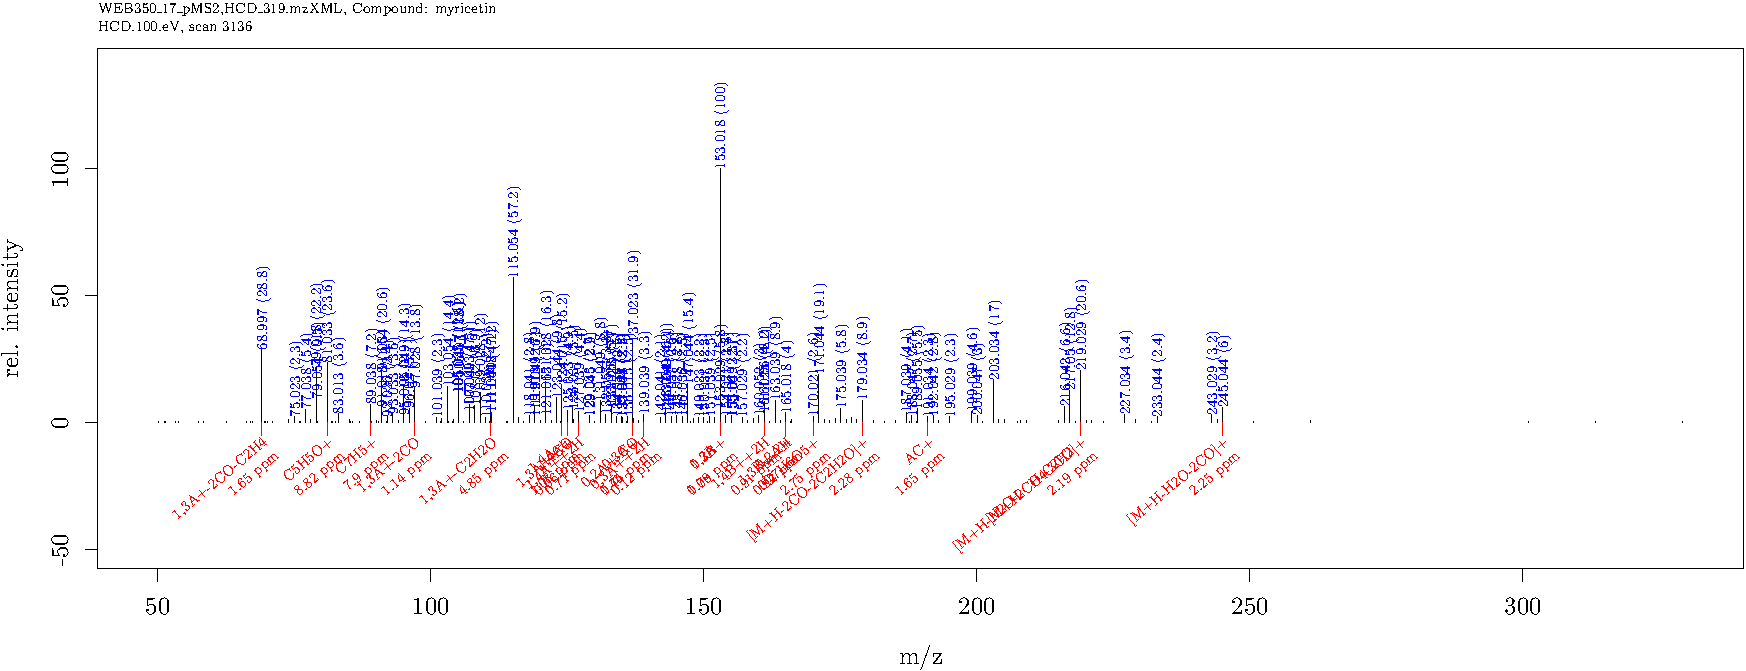
\includegraphics[width=\textwidth]{WEB350_files/figure-latex/unnamed-chunk-3-33}

\begin{table}[ht]
\centering
\begin{tabular}{rrrrl}
  \toprule
 & mz & int & ppm & fragment \\ 
  \midrule
1 & 69.00 & 28.8 & 1.65 & 1,3A+-2CO-C2H4 \\ 
  2 & 81.03 & 23.6 & 8.82 & C5H5O+ \\ 
  3 & 89.04 & 7.2 & 7.90 & C7H5+ \\ 
  4 & 97.03 & 13.8 & 1.14 & 1,3A+-2CO \\ 
  5 & 111.01 & 7.2 & 4.85 & 1,3A+-C2H2O \\ 
  6 & 124.02 & 15.2 & 1.08 & 1,4A.+ \\ 
  7 & 125.02 & 4.9 & 0.06 & 1,3A+-CO \\ 
  8 & 125.02 & 4.9 & 0.06 & 1,4A+ \\ 
  9 & 127.04 & 4.4 & 0.71 & 1,4A++2H \\ 
  10 & 137.02 & 31.9 & 1.75 & 0,2A+-CO \\ 
  11 & 137.02 & 31.9 & 0.44 & 0,3A+ \\ 
  12 & 139.04 & 3.3 & 0.12 & 0,3A++2H \\ 
  13 & 153.02 & 100.0 & 1.79 & 0,2B+ \\ 
  14 & 153.02 & 100.0 & 0.08 & 1,3A+ \\ 
  15 & 161.02 & 4.1 & 0.91 & 1,4B++2H \\ 
  16 & 165.02 & 4.0 & 0.40 & 0,2A+ \\ 
  17 & 165.02 & 4.0 & 0.92 & 1,3B+-2H \\ 
  18 & 170.02 & 2.6 & 2.75 & C7H6O5+ \\ 
  19 & 179.03 & 8.9 & 2.28 & [M+H-2CO-2C2H2O]+ \\ 
  20 & 191.03 & 2.3 & 1.65 & AC+ \\ 
  21 & 191.03 & 2.3 & 4.45 & [M+H-CH4-4CO]+ \\ 
  22 & 219.03 & 20.6 & 2.19 & [M+H-CH4-3CO]+ \\ 
  23 & 219.03 & 20.6 & 2.19 & [M+H-H2O-2CO-C2H2]+ \\ 
  24 & 245.04 & 6.0 & 2.25 & [M+H-H2O-2CO]+ \\ 
   \bottomrule
\end{tabular}
\end{table}

\clearpage\subsection{ponciretin.CID.45eV}
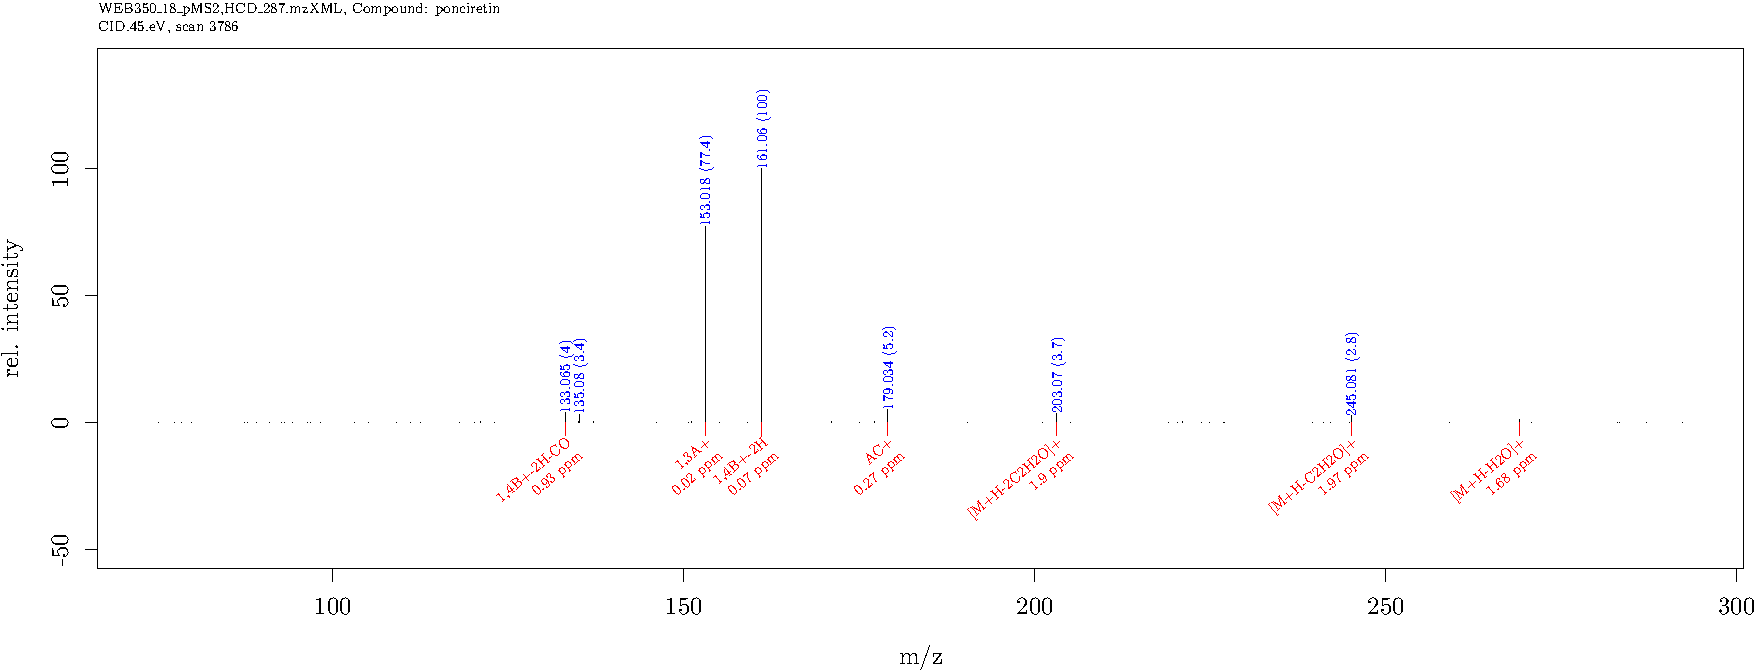
\includegraphics[width=\textwidth]{WEB350_files/figure-latex/unnamed-chunk-3-34}

\begin{table}[ht]
\centering
\begin{tabular}{rrrrl}
  \toprule
 & mz & int & ppm & fragment \\ 
  \midrule
1 & 133.06 & 4.0 & 0.93 & 1,4B+-2H-CO \\ 
  2 & 153.02 & 77.4 & 0.02 & 1,3A+ \\ 
  3 & 161.06 & 100.0 & 0.07 & 1,4B+-2H \\ 
  4 & 179.03 & 5.2 & 0.27 & AC+ \\ 
  5 & 203.07 & 3.7 & 1.90 & [M+H-2C2H2O]+ \\ 
  6 & 245.08 & 2.8 & 1.97 & [M+H-C2H2O]+ \\ 
  7 & 269.08 & 1.3 & 1.68 & [M+H-H2O]+ \\ 
   \bottomrule
\end{tabular}
\end{table}

\clearpage\subsection{ponciretin.HCD.75eV}
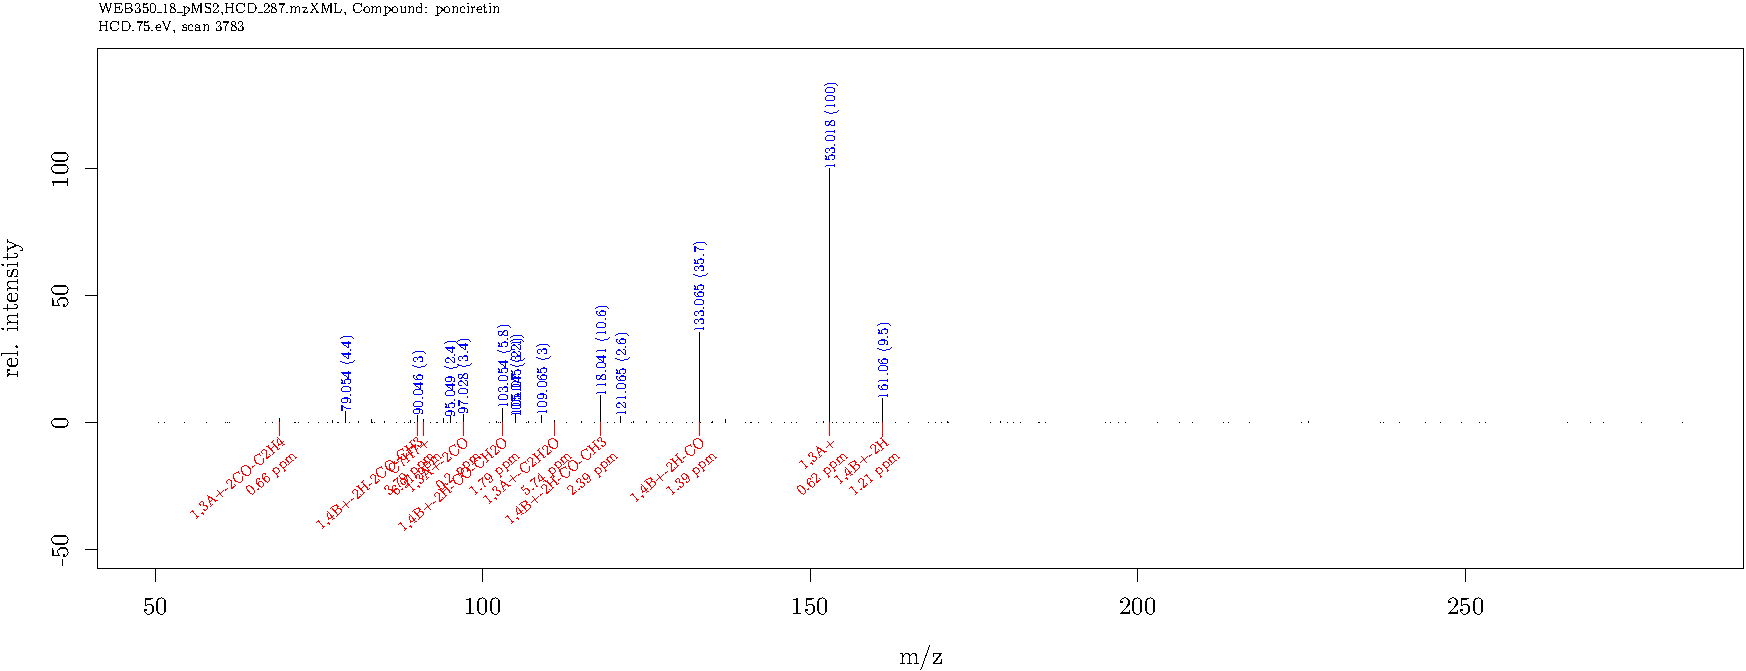
\includegraphics[width=\textwidth]{WEB350_files/figure-latex/unnamed-chunk-3-35}

\begin{table}[ht]
\centering
\begin{tabular}{rrrrl}
  \toprule
 & mz & int & ppm & fragment \\ 
  \midrule
1 & 69.00 & 1.6 & 0.66 & 1,3A+-2CO-C2H4 \\ 
  2 & 90.05 & 3.0 & 3.79 & 1,4B+-2H-2CO-CH3 \\ 
  3 & 91.05 & 1.1 & 6.91 & C7H7+ \\ 
  4 & 97.03 & 3.4 & 0.20 & 1,3A+-2CO \\ 
  5 & 103.05 & 5.8 & 1.79 & 1,4B+-2H-CO-CH2O \\ 
  6 & 111.01 & 1.1 & 5.74 & 1,3A+-C2H2O \\ 
  7 & 118.04 & 10.6 & 2.39 & 1,4B+-2H-CO-CH3 \\ 
  8 & 133.06 & 35.7 & 1.39 & 1,4B+-2H-CO \\ 
  9 & 153.02 & 100.0 & 0.62 & 1,3A+ \\ 
  10 & 161.06 & 9.5 & 1.21 & 1,4B+-2H \\ 
   \bottomrule
\end{tabular}
\end{table}

\clearpage\subsection{ponciretin.HCD.100eV}
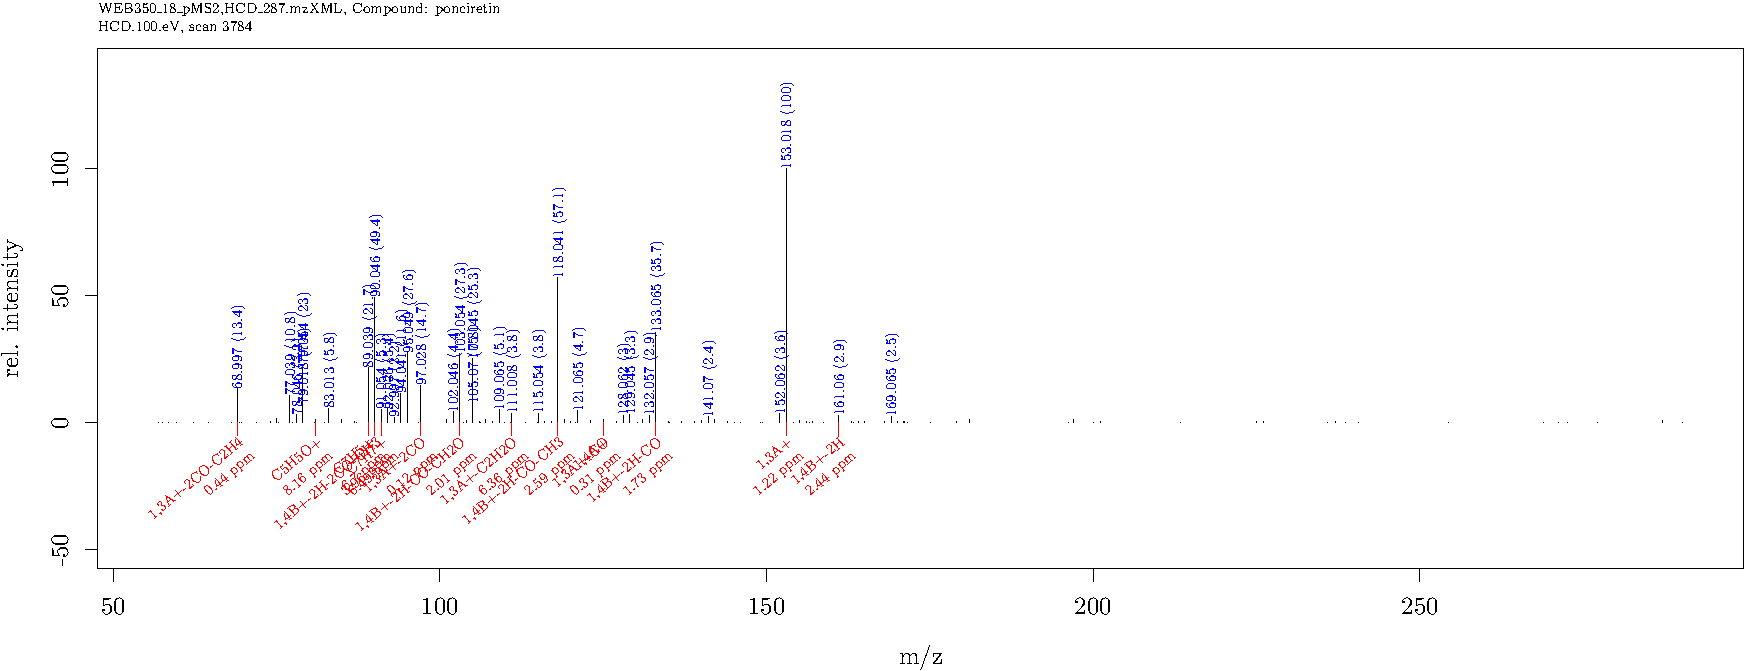
\includegraphics[width=\textwidth]{WEB350_files/figure-latex/unnamed-chunk-3-36}

\begin{table}[ht]
\centering
\begin{tabular}{rrrrl}
  \toprule
 & mz & int & ppm & fragment \\ 
  \midrule
1 & 69.00 & 13.4 & 0.44 & 1,3A+-2CO-C2H4 \\ 
  2 & 81.03 & 1.3 & 8.16 & C5H5O+ \\ 
  3 & 89.04 & 21.7 & 6.70 & C7H5+ \\ 
  4 & 90.05 & 49.4 & 3.96 & 1,4B+-2H-2CO-CH3 \\ 
  5 & 91.05 & 5.3 & 6.49 & C7H7+ \\ 
  6 & 97.03 & 14.7 & 0.12 & 1,3A+-2CO \\ 
  7 & 103.05 & 27.3 & 2.01 & 1,4B+-2H-CO-CH2O \\ 
  8 & 111.01 & 3.8 & 6.36 & 1,3A+-C2H2O \\ 
  9 & 118.04 & 57.1 & 2.59 & 1,4B+-2H-CO-CH3 \\ 
  10 & 125.02 & 1.3 & 0.31 & 1,3A+-CO \\ 
  11 & 125.02 & 1.3 & 0.31 & 1,4A+ \\ 
  12 & 133.06 & 35.7 & 1.73 & 1,4B+-2H-CO \\ 
  13 & 153.02 & 100.0 & 1.22 & 1,3A+ \\ 
  14 & 161.06 & 2.9 & 2.44 & 1,4B+-2H \\ 
   \bottomrule
\end{tabular}
\end{table}

\clearpage\subsection{acacetin.CID.45eV}
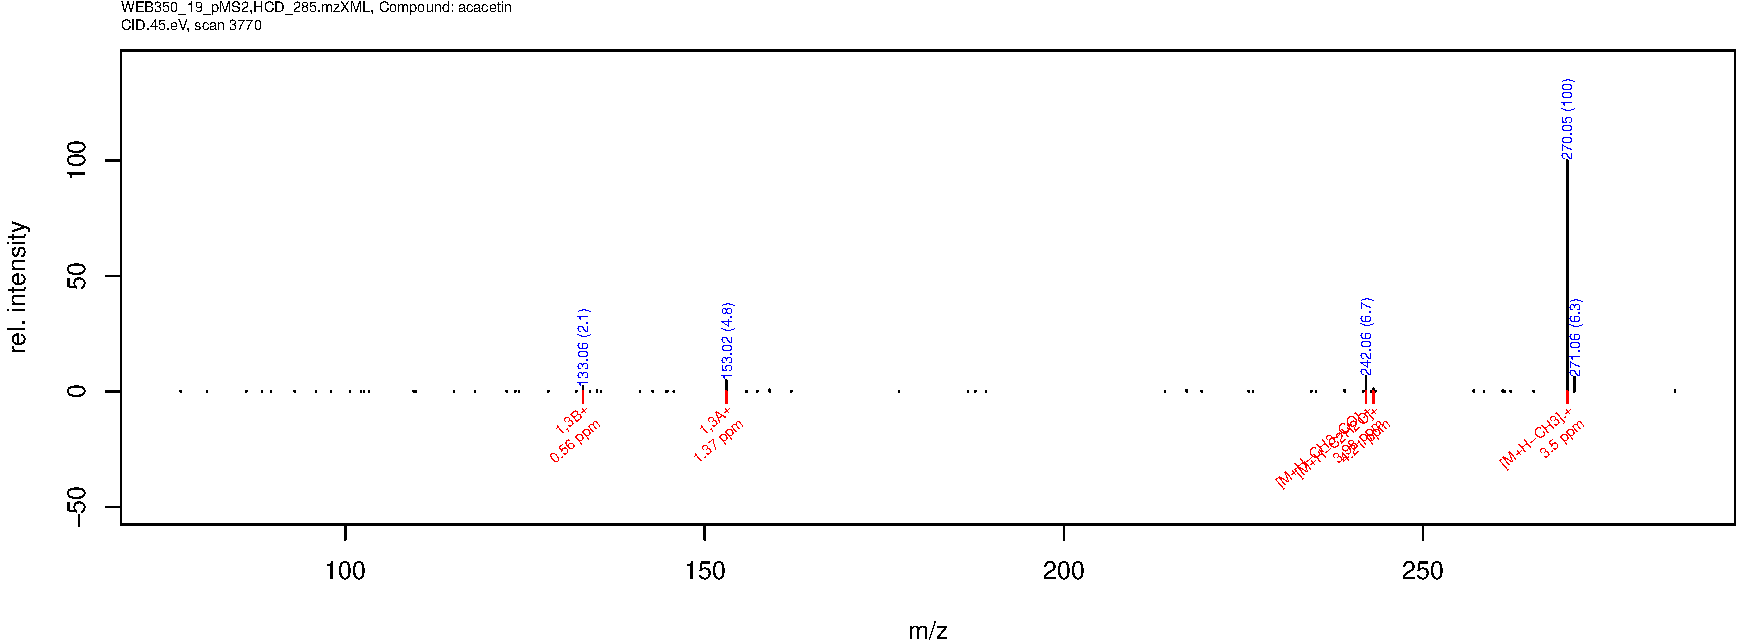
\includegraphics[width=\textwidth]{WEB350_files/figure-latex/unnamed-chunk-3-37}

\begin{table}[ht]
\centering
\begin{tabular}{rrrrl}
  \toprule
 & mz & int & ppm & fragment \\ 
  \midrule
1 & 133.06 & 2.1 & 0.56 & 1,3B+ \\ 
  2 & 153.02 & 4.8 & 1.37 & 1,3A+ \\ 
  3 & 242.06 & 6.7 & 3.98 & [M+H-CH3-CO].+ \\ 
  4 & 243.06 & 1.2 & 4.21 & [M+H-C2H2O]+ \\ 
  5 & 270.05 & 100.0 & 3.50 & [M+H-CH3].+ \\ 
   \bottomrule
\end{tabular}
\end{table}

\clearpage\subsection{acacetin.HCD.75eV}
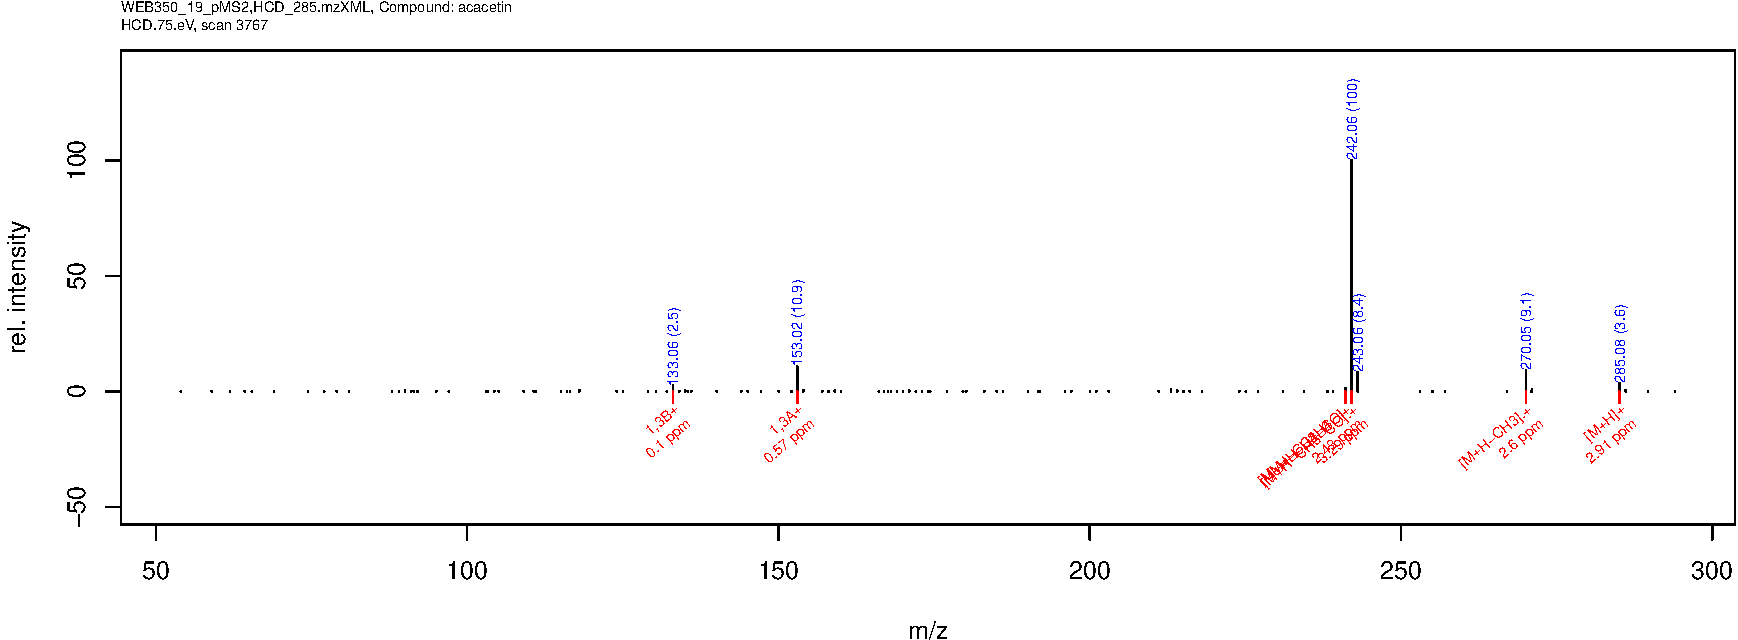
\includegraphics[width=\textwidth]{WEB350_files/figure-latex/unnamed-chunk-3-38}

\begin{table}[ht]
\centering
\begin{tabular}{rrrrl}
  \toprule
 & mz & int & ppm & fragment \\ 
  \midrule
1 & 133.06 & 2.5 & 0.10 & 1,3B+ \\ 
  2 & 153.02 & 10.9 & 0.57 & 1,3A+ \\ 
  3 & 241.05 & 1.4 & 2.43 & [M+H-CH4-CO]+ \\ 
  4 & 242.06 & 100.0 & 3.29 & [M+H-CH3-CO].+ \\ 
  5 & 270.05 & 9.1 & 2.60 & [M+H-CH3].+ \\ 
  6 & 285.08 & 3.6 & 2.91 & [M+H]+ \\ 
   \bottomrule
\end{tabular}
\end{table}

\clearpage\subsection{acacetin.HCD.100eV}
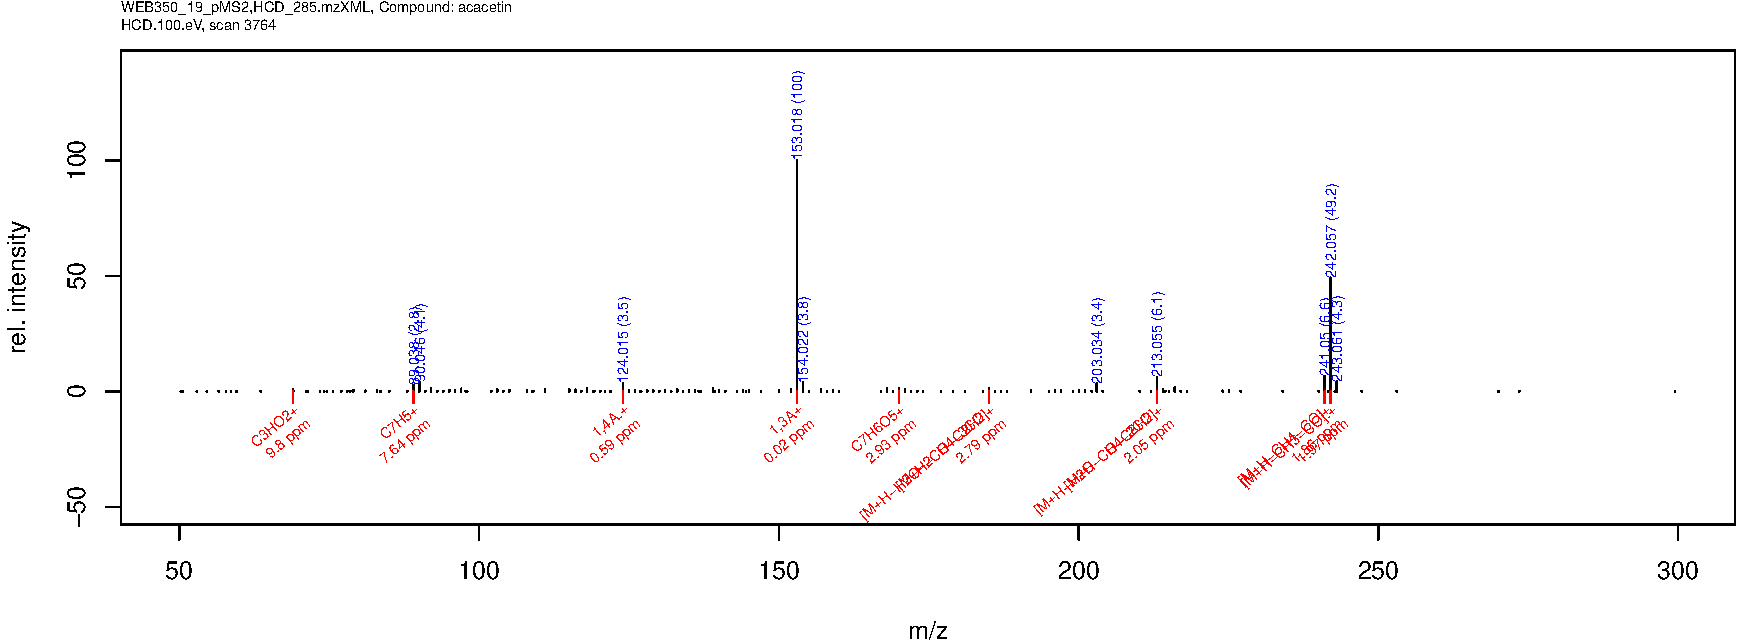
\includegraphics[width=\textwidth]{WEB350_files/figure-latex/unnamed-chunk-3-39}

\begin{table}[ht]
\centering
\begin{tabular}{rrrrl}
  \toprule
 & mz & int & ppm & fragment \\ 
  \midrule
1 & 69.00 & 1.1 & 1.32 & 1,3A+-2CO-C2H4 \\ 
  2 & 89.04 & 2.8 & 7.64 & C7H5+ \\ 
  3 & 97.03 & 1.2 & 0.91 & 1,3A+-2CO \\ 
  4 & 124.02 & 3.5 & 0.59 & 1,4A.+ \\ 
  5 & 153.02 & 100.0 & 0.02 & 1,3A+ \\ 
  6 & 170.02 & 1.3 & 2.93 & C7H6O5+ \\ 
  7 & 185.06 & 1.3 & 2.79 & [M+H-CH4-3CO]+ \\ 
  8 & 185.06 & 1.3 & 2.79 & [M+H-H2O-2CO-C2H2]+ \\ 
  9 & 213.05 & 6.1 & 2.05 & [M+H-CH4-2CO]+ \\ 
  10 & 213.05 & 6.1 & 2.05 & [M+H-H2O-CO-C2H2]+ \\ 
  11 & 241.05 & 6.6 & 1.86 & [M+H-CH4-CO]+ \\ 
  12 & 242.06 & 49.2 & 1.97 & [M+H-CH3-CO].+ \\ 
   \bottomrule
\end{tabular}
\end{table}

\clearpage\subsection{isorhamnetin.CID.45eV}
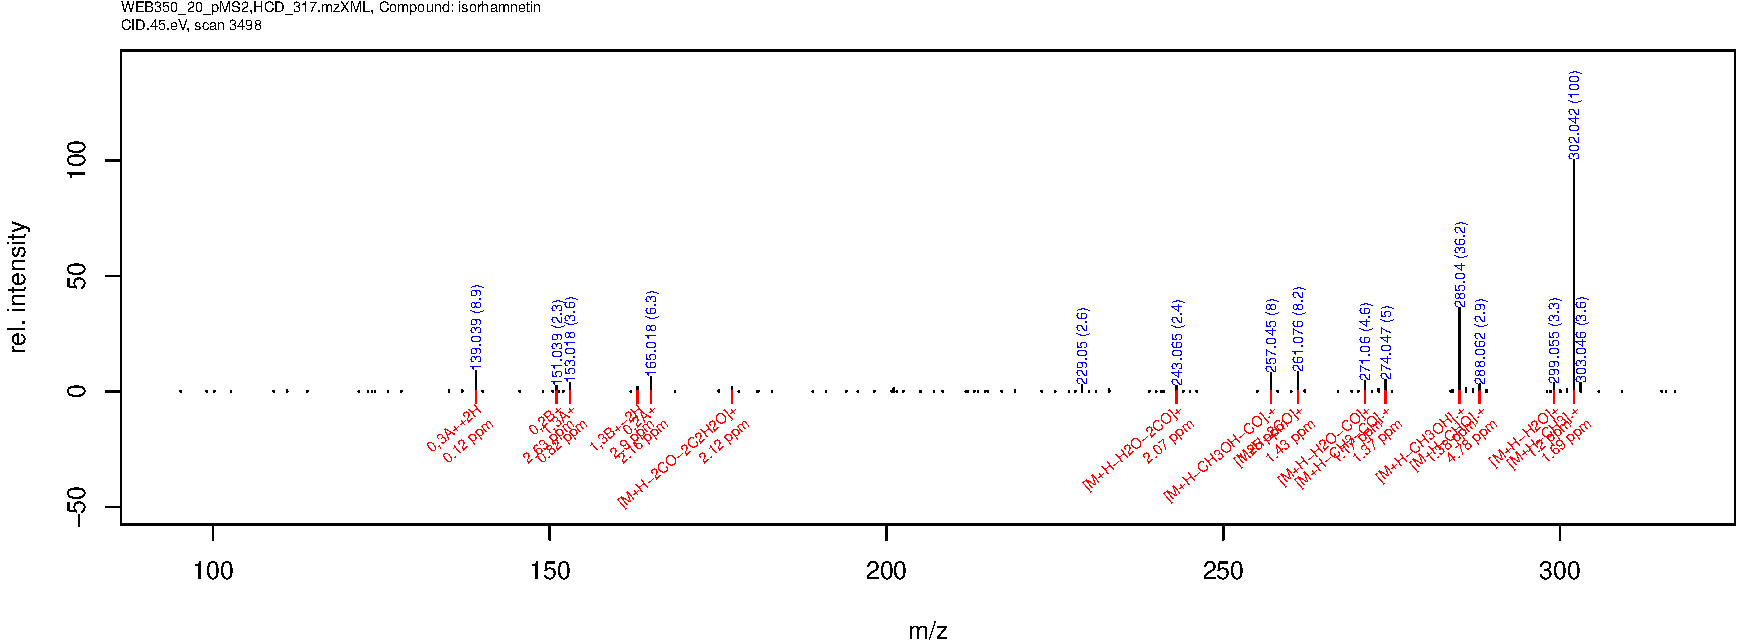
\includegraphics[width=\textwidth]{WEB350_files/figure-latex/unnamed-chunk-3-40}

\begin{table}[ht]
\centering
\begin{tabular}{rrrrl}
  \toprule
 & mz & int & ppm & fragment \\ 
  \midrule
1 & 139.04 & 8.9 & 0.12 & 0,3A++2H \\ 
  2 & 151.04 & 2.3 & 2.63 & 0,2B+ \\ 
  3 & 153.02 & 3.6 & 0.82 & 1,3A+ \\ 
  4 & 163.04 & 2.0 & 2.90 & 1,3B+-2H \\ 
  5 & 165.02 & 6.3 & 2.16 & 0,2A+ \\ 
  6 & 177.05 & 1.8 & 2.12 & [M+H-2CO-2C2H2O]+ \\ 
  7 & 229.05 & 2.6 & 1.82 & [M+H-CH3OH-2CO].+ \\ 
  8 & 243.07 & 2.4 & 2.07 & [M+H-H2O-2CO]+ \\ 
  9 & 257.04 & 8.0 & 1.25 & [M+H-CH3OH-CO].+ \\ 
  10 & 261.08 & 8.2 & 1.43 & [M+H-2CO]+ \\ 
  11 & 271.06 & 4.6 & 1.17 & [M+H-H2O-CO]+ \\ 
  12 & 274.05 & 5.0 & 1.37 & [M+H-CH3-CO].+ \\ 
  13 & 285.04 & 36.2 & 1.38 & [M+H-CH3OH].+ \\ 
  14 & 288.06 & 2.9 & 4.78 & [M+H-CHO].+ \\ 
  15 & 299.06 & 3.3 & 1.20 & [M+H-H2O]+ \\ 
  16 & 302.04 & 100.0 & 1.69 & [M+H-CH3].+ \\ 
   \bottomrule
\end{tabular}
\end{table}

\clearpage\subsection{isorhamnetin.HCD.75eV}
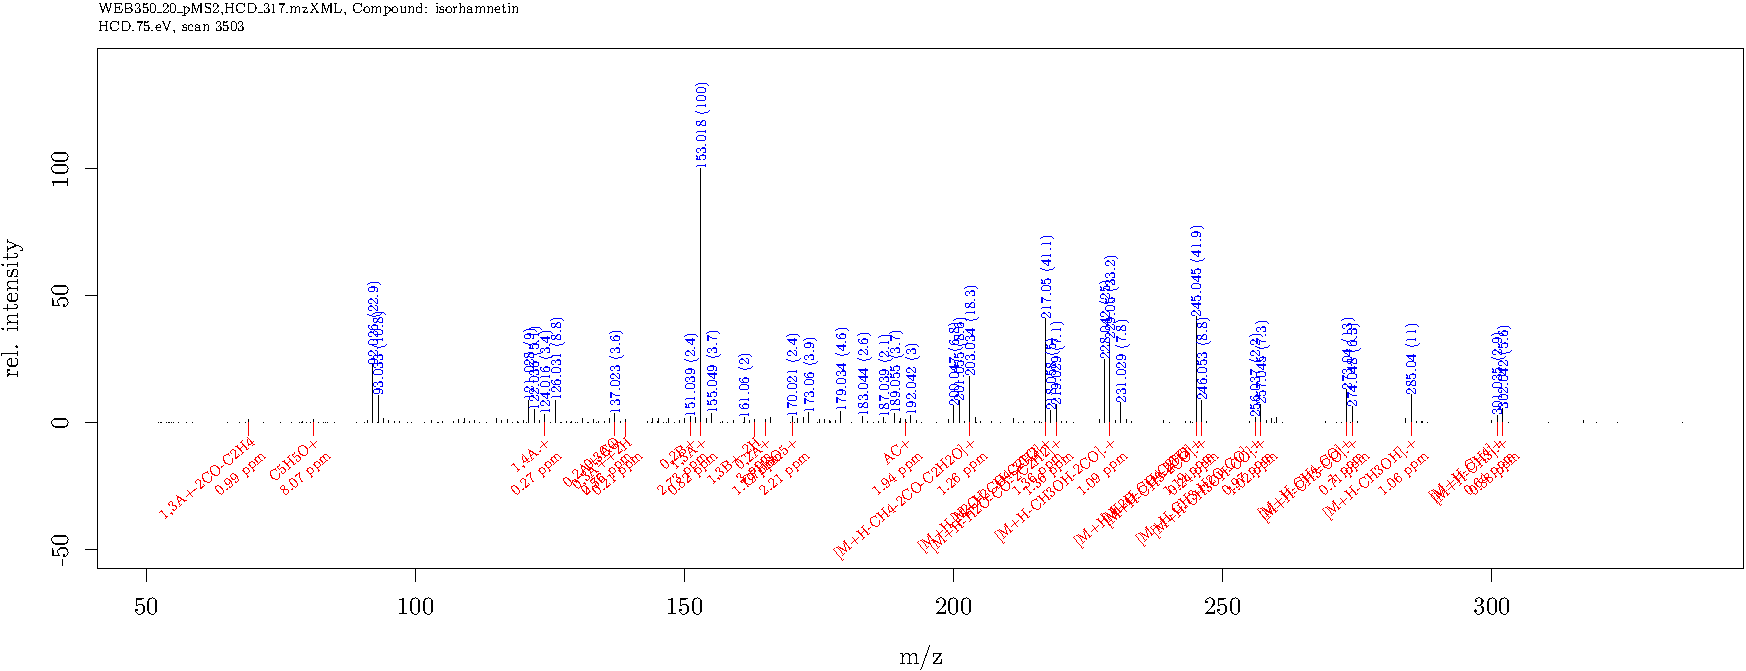
\includegraphics[width=\textwidth]{WEB350_files/figure-latex/unnamed-chunk-3-41}

\begin{table}[ht]
\centering
\begin{tabular}{rrrrl}
  \toprule
 & mz & int & ppm & fragment \\ 
  \midrule
1 & 69.00 & 1.5 & 0.99 & 1,3A+-2CO-C2H4 \\ 
  2 & 81.03 & 1.1 & 8.07 & C5H5O+ \\ 
  3 & 124.02 & 3.4 & 0.27 & 1,4A.+ \\ 
  4 & 137.02 & 3.6 & 2.75 & 0,2A+-CO \\ 
  5 & 137.02 & 3.6 & 0.56 & 0,3A+ \\ 
  6 & 139.04 & 1.3 & 0.21 & 0,3A++2H \\ 
  7 & 151.04 & 2.4 & 2.73 & 0,2B+ \\ 
  8 & 153.02 & 100.0 & 0.82 & 1,3A+ \\ 
  9 & 163.04 & 1.2 & 3.00 & 1,3B+-2H \\ 
  10 & 165.02 & 1.3 & 1.79 & 0,2A+ \\ 
  11 & 170.02 & 2.4 & 2.21 & C7H6O5+ \\ 
  12 & 189.05 & 3.7 & 1.58 & [M+H-CH4-4CO]+ \\ 
  13 & 191.03 & 1.1 & 1.94 & AC+ \\ 
  14 & 203.03 & 18.3 & 1.26 & [M+H-CH4-2CO-C2H2O]+ \\ 
  15 & 217.05 & 41.1 & 1.36 & [M+H-CH4-3CO]+ \\ 
  16 & 217.05 & 41.1 & 1.36 & [M+H-H2O-2CO-C2H2]+ \\ 
  17 & 219.03 & 7.1 & 1.36 & [M+H-H2O-CO-2C2H2]+ \\ 
  18 & 229.05 & 33.2 & 1.09 & [M+H-CH3OH-2CO].+ \\ 
  19 & 245.04 & 41.9 & 1.19 & [M+H-CH4-2CO]+ \\ 
  20 & 245.04 & 41.9 & 1.19 & [M+H-H2O-CO-C2H2]+ \\ 
  21 & 246.05 & 8.8 & 0.24 & [M+H-CH3-2CO].+ \\ 
  22 & 256.04 & 2.2 & 0.97 & [M+H-CH3-H2O-CO].+ \\ 
  23 & 257.04 & 7.3 & 1.02 & [M+H-CH3OH-CO].+ \\ 
  24 & 273.04 & 13.0 & 1.00 & [M+H-CH4-CO]+ \\ 
  25 & 274.05 & 6.3 & 0.71 & [M+H-CH3-CO].+ \\ 
  26 & 285.04 & 11.0 & 1.06 & [M+H-CH3OH].+ \\ 
  27 & 301.03 & 2.9 & 0.64 & [M+H-CH4]+ \\ 
  28 & 302.04 & 5.6 & 0.88 & [M+H-CH3].+ \\ 
   \bottomrule
\end{tabular}
\end{table}

\clearpage\subsection{isorhamnetin.HCD.100eV}
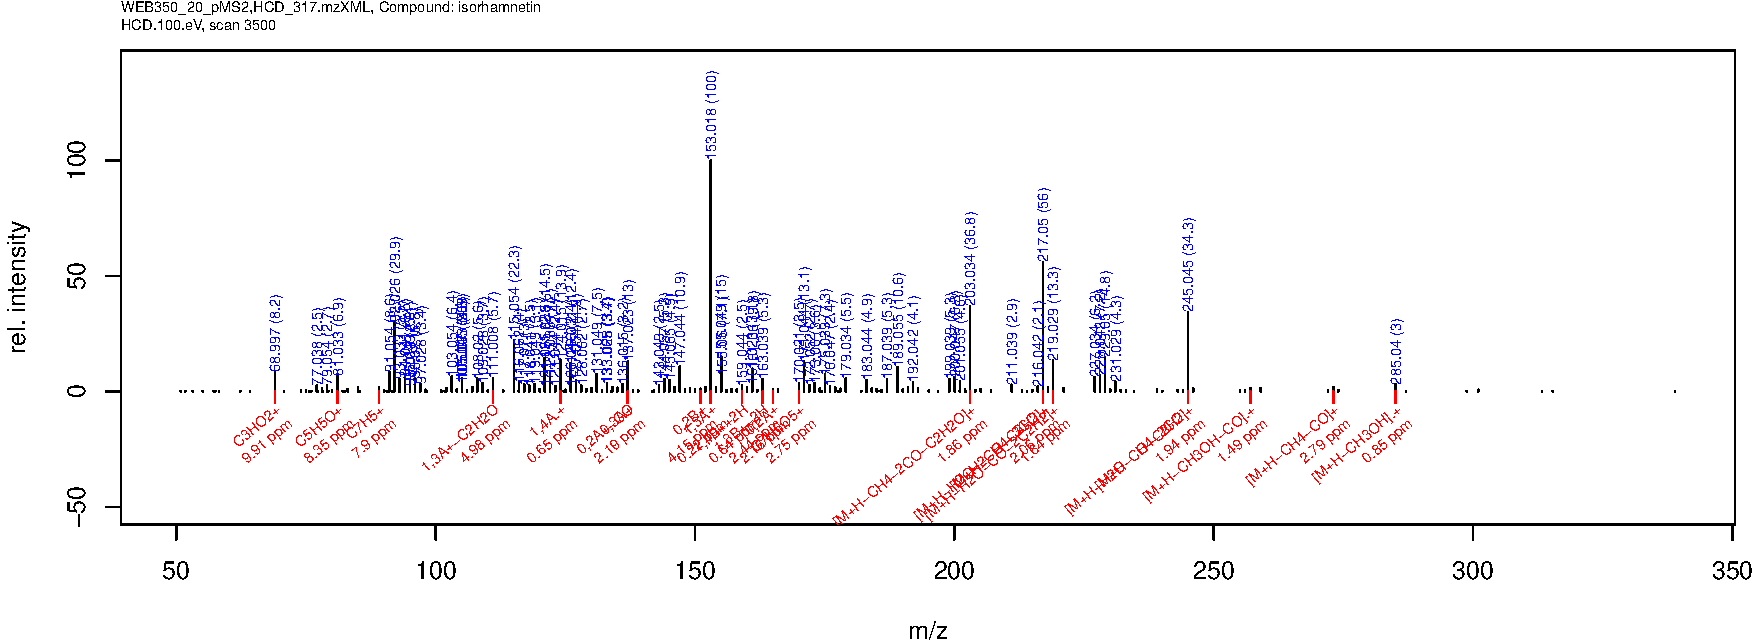
\includegraphics[width=\textwidth]{WEB350_files/figure-latex/unnamed-chunk-3-42}

\begin{table}[ht]
\centering
\begin{tabular}{rrrrl}
  \toprule
 & mz & int & ppm & fragment \\ 
  \midrule
1 & 69.00 & 8.2 & 1.43 & 1,3A+-2CO-C2H4 \\ 
  2 & 81.03 & 6.9 & 8.35 & C5H5O+ \\ 
  3 & 89.04 & 1.9 & 7.90 & C7H5+ \\ 
  4 & 97.03 & 3.4 & 0.83 & 1,3A+-2CO \\ 
  5 & 111.01 & 5.7 & 4.98 & 1,3A+-C2H2O \\ 
  6 & 124.02 & 13.9 & 0.65 & 1,4A.+ \\ 
  7 & 137.02 & 13.0 & 2.19 & 0,2A+-CO \\ 
  8 & 137.02 & 13.0 & 0.00 & 0,3A+ \\ 
  9 & 151.04 & 1.2 & 4.15 & 0,2B+ \\ 
  10 & 153.02 & 100.0 & 0.22 & 1,3A+ \\ 
  11 & 159.04 & 2.5 & 0.64 & 1,4B++2H \\ 
  12 & 163.04 & 5.3 & 2.44 & 1,3B+-2H \\ 
  13 & 165.02 & 1.0 & 2.16 & 0,2A+ \\ 
  14 & 170.02 & 3.5 & 2.75 & C7H6O5+ \\ 
  15 & 189.05 & 10.6 & 2.23 & [M+H-CH4-4CO]+ \\ 
  16 & 191.03 & 1.9 & 1.22 & AC+ \\ 
  17 & 203.03 & 36.8 & 1.86 & [M+H-CH4-2CO-C2H2O]+ \\ 
  18 & 217.05 & 56.0 & 2.06 & [M+H-CH4-3CO]+ \\ 
  19 & 217.05 & 56.0 & 2.06 & [M+H-H2O-2CO-C2H2]+ \\ 
  20 & 219.03 & 13.3 & 1.64 & [M+H-H2O-CO-2C2H2]+ \\ 
  21 & 229.05 & 14.8 & 2.02 & [M+H-CH3OH-2CO].+ \\ 
  22 & 245.04 & 34.3 & 1.94 & [M+H-CH4-2CO]+ \\ 
  23 & 245.04 & 34.3 & 1.94 & [M+H-H2O-CO-C2H2]+ \\ 
  24 & 257.04 & 1.6 & 1.49 & [M+H-CH3OH-CO].+ \\ 
  25 & 273.04 & 1.9 & 2.79 & [M+H-CH4-CO]+ \\ 
  26 & 285.04 & 3.0 & 0.85 & [M+H-CH3OH].+ \\ 
   \bottomrule
\end{tabular}
\end{table}

\clearpage\subsection{kaempferide.CID.45eV}
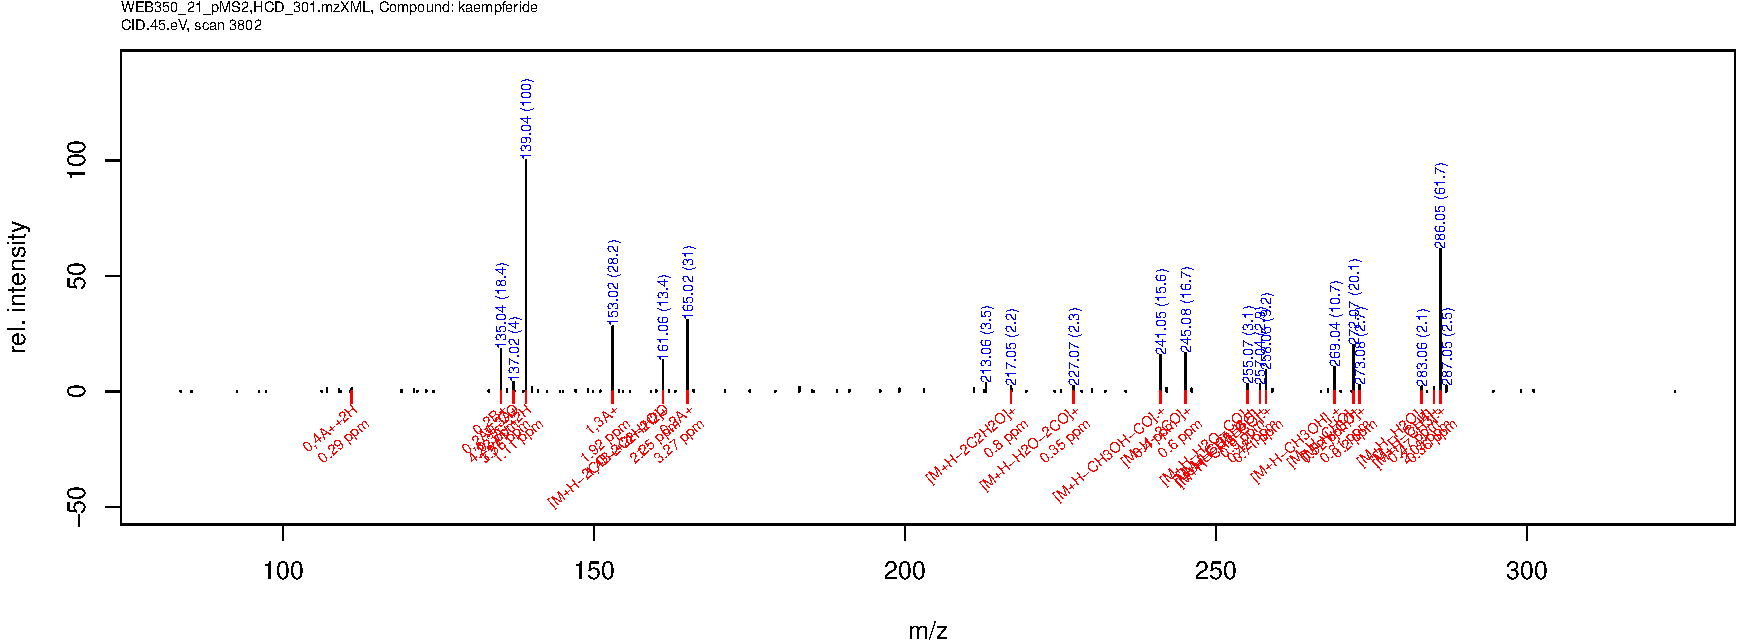
\includegraphics[width=\textwidth]{WEB350_files/figure-latex/unnamed-chunk-3-43}

\begin{table}[ht]
\centering
\begin{tabular}{rrrrl}
  \toprule
 & mz & int & ppm & fragment \\ 
  \midrule
1 & 111.04 & 1.3 & 0.29 & 0,4A++2H \\ 
  2 & 135.04 & 18.4 & 4.22 & 0,2B+ \\ 
  3 & 137.02 & 4.0 & 3.75 & 0,2A+-CO \\ 
  4 & 137.02 & 4.0 & 1.56 & 0,3A+ \\ 
  5 & 139.04 & 100.0 & 1.11 & 0,3A++2H \\ 
  6 & 153.02 & 28.2 & 1.92 & 1,3A+ \\ 
  7 & 161.06 & 13.4 & 2.25 & 1,4B++2H-H2O \\ 
  8 & 161.06 & 13.4 & 1.50 & [M+H-2CO-2C2H2O]+ \\ 
  9 & 165.02 & 31.0 & 3.27 & 0,2A+ \\ 
  10 & 213.06 & 3.5 & 0.03 & [M+H-CH3OH-2CO].+ \\ 
  11 & 217.05 & 2.2 & 0.80 & [M+H-2C2H2O]+ \\ 
  12 & 227.07 & 2.3 & 0.35 & [M+H-H2O-2CO]+ \\ 
  13 & 241.05 & 15.6 & 0.40 & [M+H-CH3OH-CO].+ \\ 
  14 & 245.08 & 16.7 & 0.60 & [M+H-2CO]+ \\ 
  15 & 255.07 & 3.1 & 0.90 & [M+H-H2O-CO]+ \\ 
  16 & 257.04 & 2.9 & 0.42 & [M+H-CH4-CO]+ \\ 
  17 & 258.05 & 9.2 & 0.71 & [M+H-CH3-CO].+ \\ 
  18 & 269.04 & 10.7 & 0.52 & [M+H-CH3OH].+ \\ 
  19 & 272.07 & 20.1 & 0.31 & [M+H-CHO].+ \\ 
  20 & 273.08 & 2.7 & 0.20 & [M+H-CO]+ \\ 
  21 & 283.06 & 2.1 & 0.47 & [M+H-H2O]+ \\ 
  22 & 285.04 & 2.0 & 2.03 & [M+H-CH4]+ \\ 
  23 & 286.05 & 61.7 & 0.36 & [M+H-CH3].+ \\ 
   \bottomrule
\end{tabular}
\end{table}

\clearpage\subsection{kaempferide.HCD.75eV}
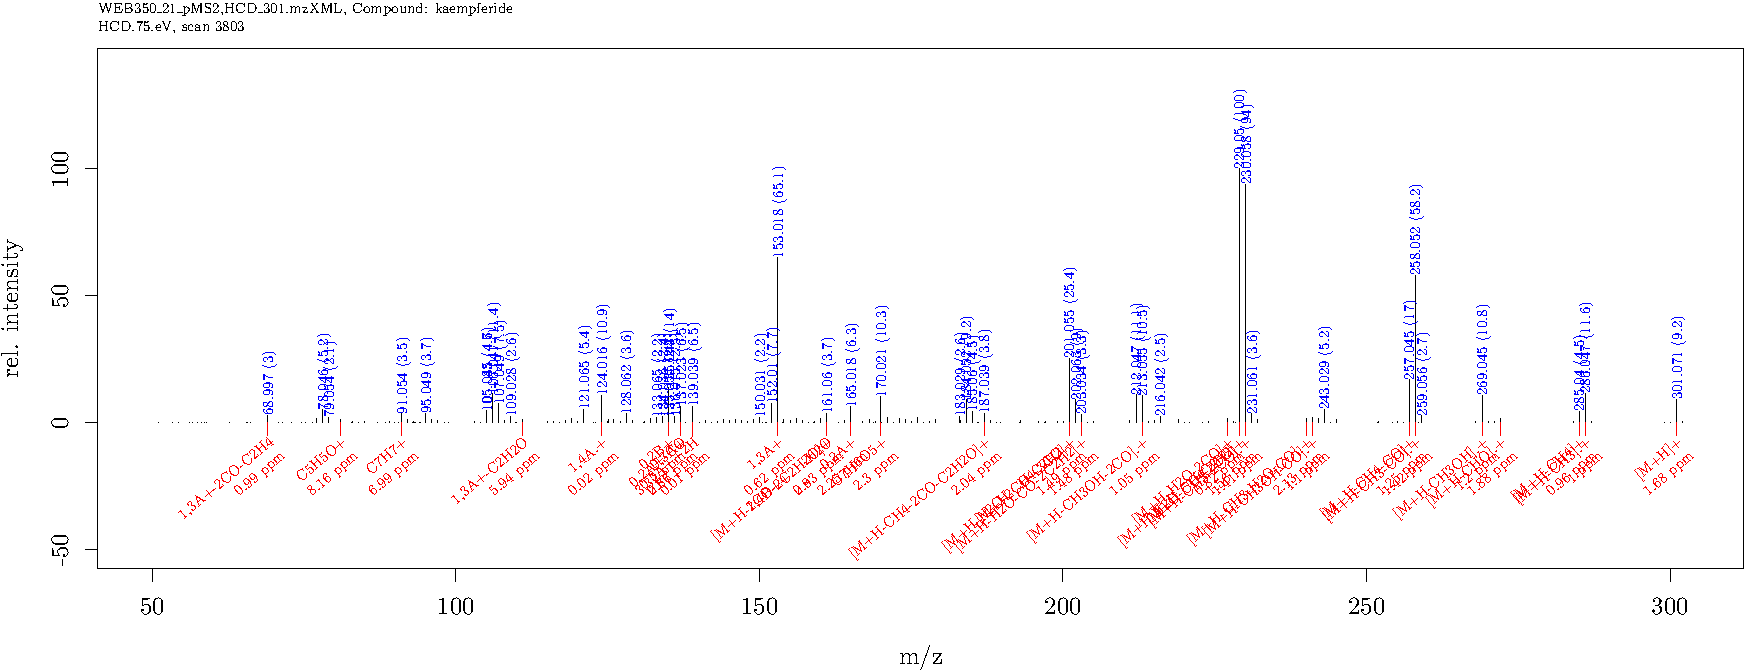
\includegraphics[width=\textwidth]{WEB350_files/figure-latex/unnamed-chunk-3-44}

\begin{table}[ht]
\centering
\begin{tabular}{rrrrl}
  \toprule
 & mz & int & ppm & fragment \\ 
  \midrule
1 & 69.00 & 3.0 & 0.99 & 1,3A+-2CO-C2H4 \\ 
  2 & 81.03 & 1.2 & 8.16 & C5H5O+ \\ 
  3 & 91.05 & 3.5 & 6.99 & C7H7+ \\ 
  4 & 111.01 & 1.2 & 5.94 & 1,3A+-C2H2O \\ 
  5 & 124.02 & 10.9 & 0.02 & 1,4A.+ \\ 
  6 & 135.04 & 14.0 & 3.32 & 0,2B+ \\ 
  7 & 137.02 & 6.5 & 2.86 & 0,2A+-CO \\ 
  8 & 137.02 & 6.5 & 0.67 & 0,3A+ \\ 
  9 & 139.04 & 6.5 & 0.01 & 0,3A++2H \\ 
  10 & 153.02 & 65.1 & 0.62 & 1,3A+ \\ 
  11 & 161.06 & 3.7 & 0.93 & 1,4B++2H-H2O \\ 
  12 & 161.06 & 3.7 & 2.83 & [M+H-2CO-2C2H2O]+ \\ 
  13 & 165.02 & 6.3 & 2.25 & 0,2A+ \\ 
  14 & 170.02 & 10.3 & 2.30 & C7H6O5+ \\ 
  15 & 173.06 & 1.9 & 2.28 & [M+H-CH4-4CO]+ \\ 
  16 & 187.04 & 3.8 & 2.04 & [M+H-CH4-2CO-C2H2O]+ \\ 
  17 & 201.05 & 25.4 & 1.49 & [M+H-CH4-3CO]+ \\ 
  18 & 201.05 & 25.4 & 1.49 & [M+H-H2O-2CO-C2H2]+ \\ 
  19 & 203.03 & 3.3 & 1.48 & [M+H-H2O-CO-2C2H2]+ \\ 
  20 & 213.05 & 10.5 & 1.05 & [M+H-CH3OH-2CO].+ \\ 
  21 & 227.07 & 1.6 & 0.82 & [M+H-H2O-2CO]+ \\ 
  22 & 229.05 & 100.0 & 1.56 & [M+H-CH4-2CO]+ \\ 
  23 & 229.05 & 100.0 & 1.56 & [M+H-H2O-CO-C2H2]+ \\ 
  24 & 230.06 & 94.0 & 1.41 & [M+H-CH3-2CO].+ \\ 
  25 & 240.04 & 1.8 & 2.13 & [M+H-CH3-H2O-CO].+ \\ 
  26 & 241.05 & 2.0 & 1.10 & [M+H-CH3OH-CO].+ \\ 
  27 & 257.04 & 17.0 & 1.25 & [M+H-CH4-CO]+ \\ 
  28 & 258.05 & 58.2 & 1.42 & [M+H-CH3-CO].+ \\ 
  29 & 269.04 & 10.8 & 1.20 & [M+H-CH3OH].+ \\ 
  30 & 272.07 & 1.8 & 1.88 & [M+H-CHO].+ \\ 
  31 & 285.04 & 4.5 & 0.96 & [M+H-CH4]+ \\ 
  32 & 286.05 & 11.6 & 1.00 & [M+H-CH3].+ \\ 
  33 & 301.07 & 9.2 & 1.68 & [M+H]+ \\ 
   \bottomrule
\end{tabular}
\end{table}

\clearpage\subsection{kaempferide.HCD.100eV}
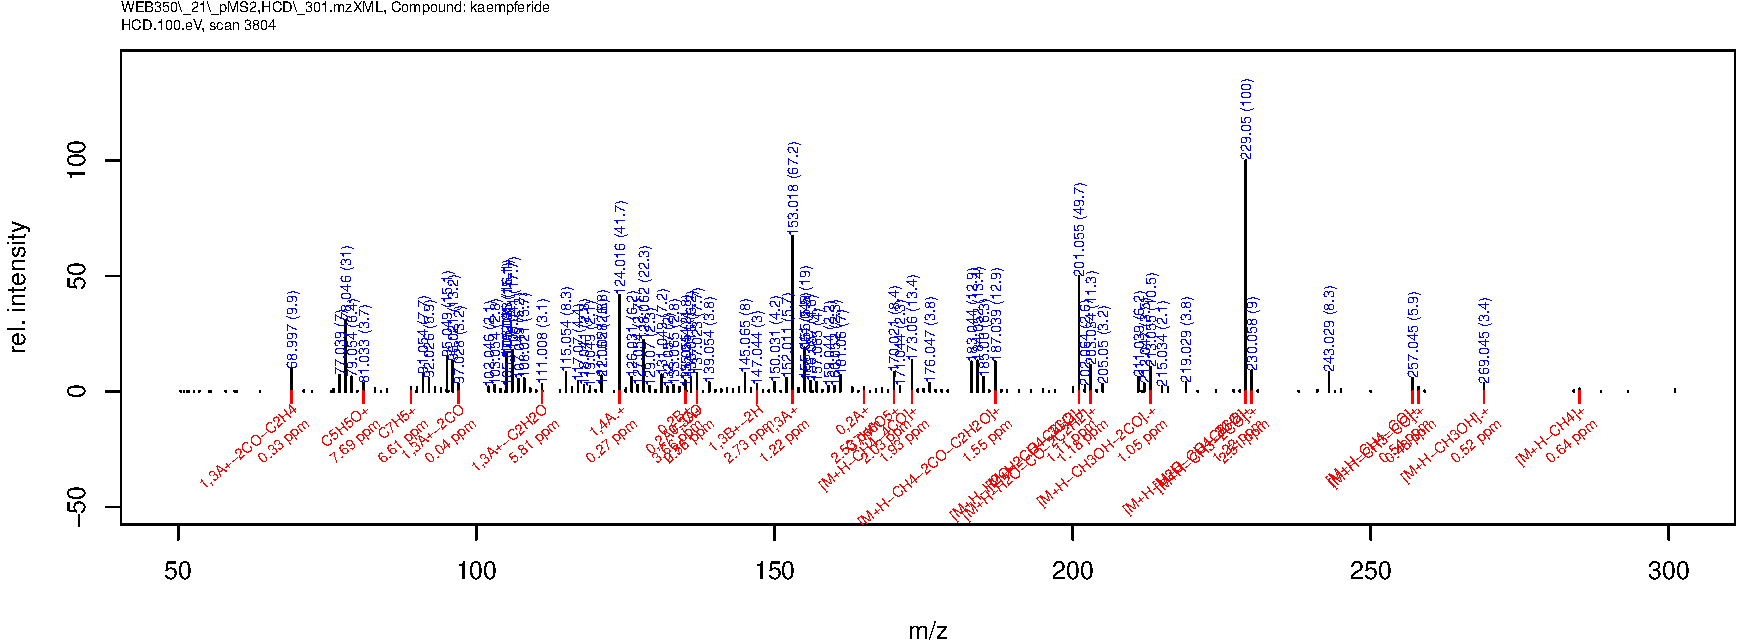
\includegraphics[width=\textwidth]{WEB350_files/figure-latex/unnamed-chunk-3-45}

\begin{table}[ht]
\centering
\begin{tabular}{rrrrl}
  \toprule
 & mz & int & ppm & fragment \\ 
  \midrule
1 & 69.00 & 9.9 & 0.33 & 1,3A+-2CO-C2H4 \\ 
  2 & 81.03 & 3.7 & 7.69 & C5H5O+ \\ 
  3 & 89.04 & 1.8 & 6.61 & C7H5+ \\ 
  4 & 97.03 & 3.2 & 0.04 & 1,3A+-2CO \\ 
  5 & 111.01 & 3.1 & 5.81 & 1,3A+-C2H2O \\ 
  6 & 124.02 & 41.7 & 0.27 & 1,4A.+ \\ 
  7 & 135.04 & 4.8 & 3.66 & 0,2B+ \\ 
  8 & 137.02 & 7.7 & 2.75 & 0,2A+-CO \\ 
  9 & 137.02 & 7.7 & 0.56 & 0,3A+ \\ 
  10 & 147.04 & 3.0 & 2.73 & 1,3B+-2H \\ 
  11 & 153.02 & 67.2 & 1.22 & 1,3A+ \\ 
  12 & 165.02 & 1.9 & 2.53 & 0,2A+ \\ 
  13 & 170.02 & 8.4 & 2.03 & C7H6O5+ \\ 
  14 & 173.06 & 13.4 & 1.93 & [M+H-CH4-4CO]+ \\ 
  15 & 187.04 & 12.9 & 1.55 & [M+H-CH4-2CO-C2H2O]+ \\ 
  16 & 201.05 & 49.7 & 1.11 & [M+H-CH4-3CO]+ \\ 
  17 & 201.05 & 49.7 & 1.11 & [M+H-H2O-2CO-C2H2]+ \\ 
  18 & 203.03 & 11.3 & 1.18 & [M+H-H2O-CO-2C2H2]+ \\ 
  19 & 213.05 & 10.5 & 1.05 & [M+H-CH3OH-2CO].+ \\ 
  20 & 229.05 & 100.0 & 1.22 & [M+H-CH4-2CO]+ \\ 
  21 & 229.05 & 100.0 & 1.22 & [M+H-H2O-CO-C2H2]+ \\ 
  22 & 230.06 & 9.0 & 2.51 & [M+H-CH3-2CO].+ \\ 
  23 & 257.04 & 5.9 & 0.54 & [M+H-CH4-CO]+ \\ 
  24 & 258.05 & 1.8 & 0.48 & [M+H-CH3-CO].+ \\ 
  25 & 269.04 & 3.4 & 0.52 & [M+H-CH3OH].+ \\ 
  26 & 285.04 & 1.2 & 0.64 & [M+H-CH4]+ \\ 
   \bottomrule
\end{tabular}
\end{table}

\clearpage

\setlength\tabcolsep{1.5pt}

\begin{sidewaystable}\caption{Fragment table for method \textit{CID.45}}{\scriptsize
\begin{tabular}{ll|ccccc|ccccc|ccccc}
  \toprule
 & \begin{sideways} fragment \end{sideways} & \begin{sideways} naringenin \end{sideways} & \begin{sideways} eriodictyol \end{sideways} & \begin{sideways} ponciretin \end{sideways} & \begin{sideways} hesperetin \end{sideways} & \begin{sideways} homoeriodictyol \end{sideways} & \begin{sideways} apigenin \end{sideways} & \begin{sideways} luteolin \end{sideways} & \begin{sideways} acacetin \end{sideways} & \begin{sideways} diosmetin \end{sideways} & \begin{sideways} chrysoeriol \end{sideways} & \begin{sideways} kaempferol \end{sideways} & \begin{sideways} quercetin \end{sideways} & \begin{sideways} myricetin \end{sideways} & \begin{sideways} kaempferide \end{sideways} & \begin{sideways} isorhamnetin \end{sideways} \\ 
  \midrule
1 & $\mathrm{[M{+}H]^+}$ &  &  &  &  &  & 271\,(2) &  &  &  &  &  &  &  &  &  \\ 
  2 & $\mathrm{[M{+}H{-}CH_{3}]^{\bullet+}}$ &  &  &  &  &  &  &  & 270\,(100) & 286\,(100) & 286\,(100) &  &  &  & 286\,(62) & 302\,(100) \\ 
  3 & $\mathrm{[M{+}H{-}CH_{4}]^+}$ &  &  &  &  &  &  &  &  &  &  &  &  &  & 285\,(2) &  \\ 
  4 & $\mathrm{[M{+}H{-}H_{2}O]^+}$ & 255\,(1) & 271\,(18) & 269\,(1) & 285\,(10) & 285\,(4) & 253\,(1) & 269\,(9) &  &  &  & 269\,(32) & 285\,(63) & 301\,(40) & 283\,(2) & 299\,(3) \\ 
  5 & $\mathrm{[M{+}H{-}CO]^+}$ &  &  &  &  &  & 243\,(7) & 259\,(9) &  &  &  & 259\,(24) & 275\,(14) & 291\,(6) & 273\,(3) &  \\ 
  6 & $\mathrm{[M{+}H{-}CHO]^{\bullet+}}$ &  &  &  &  &  & 242\,(14) & 258\,(47) &  &  &  & 258\,(46) & 274\,(20) & 290\,(22) & 272\,(20) & 288\,(3) \\ 
  7 & $\mathrm{[M{+}H{-}CH_{3}OH]^{\bullet+}}$ &  &  &  &  &  &  &  &  &  &  &  &  &  & 269\,(11) & 285\,(36) \\ 
  8 & $\mathrm{[M{+}H{-}2H_{2}O]^+}$ &  & 253\,(4) &  &  &  &  &  &  &  &  &  &  & 283\,(4) &  &  \\ 
  9 & $\mathrm{[M{+}H{-}C_{2}H_{2}O]^+}$ & 231\,(4) & 247\,(3) & 245\,(3) & 261\,(2) & 261\,(2) & 229\,(21) & 245\,(13) & 243\,(1) &  &  & 245\,(4) &  &  &  &  \\ 
  10 & $\mathrm{[M{+}H{-}CH_{3}{-}CO]^{\bullet+}}$ &  &  &  &  &  &  &  & 242\,(7) &  &  &  &  &  & 258\,(9) & 274\,(5) \\ 
  11 & $\mathrm{[M{+}H{-}CO_{2}]^+}$ &  &  &  &  &  &  &  &  &  &  & 243\,(5) &  &  &  &  \\ 
  12 & $\mathrm{[M{+}H{-}CH_{4}{-}CO]^+}$ &  &  &  &  &  &  &  &  &  &  &  &  &  & 257\,(3) &  \\ 
  13 & $\mathrm{[M{+}H{-}H_{2}O{-}CO]^+}$ &  &  &  &  &  & 225\,(13) & 241\,(13) &  &  &  & 241\,(99) & 257\,(100) & 273\,(100) & 255\,(3) & 271\,(5) \\ 
  14 & $\mathrm{[M{+}H{-}2CO]^+}$ &  &  &  &  &  &  & 231\,(2) &  &  &  & 231\,(40) & 247\,(37) & 263\,(25) & 245\,(17) & 261\,(8) \\ 
  15 & $\mathrm{[M{+}H{-}CH_{3}OH{-}CO]^{\bullet+}}$ &  &  &  &  &  &  & 227\,(3) &  &  &  &  &  &  & 241\,(16) & 257\,(8) \\ 
  16 & $\mathrm{[M{+}H{-}H_{2}O{-}2CO]^+}$ &  &  &  &  &  &  & 213\,(2) &  &  &  & 213\,(77) & 229\,(70) & 245\,(32) & 227\,(2) & 243\,(2) \\ 
  17 & $\mathrm{[M{+}H{-}2C_{2}H_{2}O]^+}$ & 189\,(5) & 205\,(3) & 203\,(4) & 219\,(2) & 219\,(1) & 187\,(3) & 203\,(4) &  &  &  & 203\,(7) & 219\,(4) & 235\,(4) & 217\,(2) &  \\ 
  18 & $\mathrm{[M{+}H{-}CH_{3}OH{-}2CO]^{\bullet+}}$ &  &  &  &  &  &  &  &  &  &  & 199\,(3) & 215\,(2) & 231\,(2) & 213\,(4) & 229\,(3) \\ 
  19 & $\mathrm{[M{+}H{-}2C_{2}H_{2}O{-}H_{2}O]^+}$ &  & 187\,(4) &  & 201\,(1) &  &  &  &  &  &  &  &  &  &  &  \\ 
  20 & $\mathrm{[M{+}H{-}CH_{4}{-}4CO]^+}$ &  & 161\,(2) &  &  &  &  &  &  &  &  &  &  &  &  &  \\ 
  21 & $\mathrm{[M{+}H{-}2CO{-}2C_{2}H_{2}O]^+}$ &  &  &  &  &  &  &  &  &  &  & 147\,(13) & 163\,(7) & 179\,(7) & 161\,(13) & 177\,(2) \\ 
  22 & $\mathrm{AC^+}$ & 179\,(4) & 179\,(20) & 179\,(5) & 179\,(28) & 179\,(30) &  &  &  &  &  &  & 191\,(1) &  &  &  \\ 
  23 & $\mathrm{0{,}2A^+}$ &  &  &  &  &  &  &  &  &  &  & 165\,(100) & 165\,(59) & 165\,(41) & 165\,(31) & 165\,(6) \\ 
  24 & $\mathrm{0{,}2A^+{-}CO}$ &  &  &  &  &  &  &  &  &  &  & 137\,(11) & 137\,(23) & 137\,(6) & 137\,(4) &  \\ 
  25 & $\mathrm{0{,}2B^+}$ &  &  &  &  &  & 121\,(6) & 137\,(7) &  &  &  & 121\,(36) & 137\,(23) & 153\,(35) & 135\,(18) & 151\,(2) \\ 
  26 & $\mathrm{0{,}3A^+}$ &  &  &  &  &  &  & 137\,(7) &  &  &  & 137\,(11) & 137\,(23) & 137\,(6) & 137\,(4) &  \\ 
  27 & $\mathrm{0{,}3A^+{+}2H}$ &  &  &  &  &  &  &  &  &  &  &  &  &  & 139\,(100) & 139\,(9) \\ 
  28 & $\mathrm{0{,}4A^+{+}2H}$ &  &  &  &  &  &  &  &  &  &  &  &  &  & 111\,(1) &  \\ 
  29 & $\mathrm{0{,}4B^+}$ &  &  &  &  &  & 163\,(6) & 179\,(7) &  &  &  &  &  &  &  &  \\ 
  30 & $\mathrm{0{,}4B^+{-}H_{2}O}$ &  &  &  &  &  & 145\,(13) &  &  &  &  &  &  &  &  &  \\ 
  31 & $\mathrm{1{,}3A^+}$ & 153\,(100) & 153\,(31) & 153\,(77) & 153\,(21) & 153\,(57) & 153\,(100) & 153\,(100) & 153\,(5) &  &  & 153\,(61) & 153\,(20) & 153\,(35) & 153\,(28) & 153\,(4) \\ 
  32 & $\mathrm{1{,}3A^+{-}C_{2}H_{2}O}$ &  &  &  &  &  &  &  &  &  &  & 111\,(19) & 111\,(7) & 111\,(4) &  &  \\ 
  33 & $\mathrm{1{,}3B^+}$ &  &  &  &  &  & 119\,(12) & 135\,(11) & 133\,(2) &  &  &  &  &  &  &  \\ 
  34 & $\mathrm{1{,}3B^+{-}2H}$ &  &  &  &  &  &  &  &  &  &  & 133\,(25) & 149\,(10) & 165\,(41) &  & 163\,(2) \\ 
  35 & $\mathrm{1{,}4A^+{+}2H}$ &  &  &  &  &  &  &  &  &  &  & 127\,(2) & 127\,(1) & 127\,(4) &  &  \\ 
  36 & $\mathrm{1{,}4B^+{-}2H}$ & 147\,(84) & 163\,(100) & 161\,(100) & 177\,(100) & 177\,(100) &  &  &  &  &  &  &  &  &  &  \\ 
  37 & $\mathrm{1{,}4B^+{+}2H{-}H_{2}O}$ &  &  &  &  &  &  &  &  &  &  & 147\,(13) &  &  & 161\,(13) &  \\ 
  38 & $\mathrm{1{,}4B^+{-}2H{-}H_{2}O}$ &  & 145\,(5) &  &  &  &  &  &  &  &  &  &  &  &  &  \\ 
  39 & $\mathrm{1{,}4B^+{-}2H{-}CO}$ & 119\,(3) & 135\,(1) & 133\,(4) &  &  &  &  &  &  &  &  &  &  &  &  \\ 
  40 & $\mathrm{C_{7}H_{7}^+}$ &  &  &  &  &  & 91\,(1) &  &  &  &  &  &  &  &  &  \\ 
   \bottomrule
\end{tabular}
}
\end{sidewaystable}

\qquad

\begin{sidewaystable}\caption{Fragment table for method \textit{HCD.75}}{\scriptsize
\begin{tabular}{ll|ccccc|ccccc|ccccc}
  \toprule
 & \begin{sideways} fragment \end{sideways} & \begin{sideways} naringenin \end{sideways} & \begin{sideways} eriodictyol \end{sideways} & \begin{sideways} ponciretin \end{sideways} & \begin{sideways} hesperetin \end{sideways} & \begin{sideways} homoeriodictyol \end{sideways} & \begin{sideways} apigenin \end{sideways} & \begin{sideways} luteolin \end{sideways} & \begin{sideways} acacetin \end{sideways} & \begin{sideways} diosmetin \end{sideways} & \begin{sideways} chrysoeriol \end{sideways} & \begin{sideways} kaempferol \end{sideways} & \begin{sideways} quercetin \end{sideways} & \begin{sideways} myricetin \end{sideways} & \begin{sideways} kaempferide \end{sideways} & \begin{sideways} isorhamnetin \end{sideways} \\ 
  \midrule
1 & $\mathrm{[M{+}H]^+}$ &  &  &  &  &  & 271\,(84) & 287\,(66) & 285\,(4) &  &  & 287\,(25) & 303\,(8) & 319\,(1) & 301\,(9) &  \\ 
  2 & $\mathrm{[M{+}H{-}CH_{3}]^{\bullet+}}$ &  &  &  &  &  &  &  & 270\,(9) & 286\,(20) & 286\,(18) &  &  &  & 286\,(12) & 302\,(6) \\ 
  3 & $\mathrm{[M{+}H{-}CH_{4}]^+}$ &  &  &  & 287\,(1) &  &  &  &  &  &  &  &  &  & 285\,(5) & 301\,(3) \\ 
  4 & $\mathrm{[M{+}H{-}H_{2}O]^+}$ &  &  &  &  &  & 253\,(3) & 269\,(6) &  &  &  & 269\,(2) & 285\,(6) & 301\,(1) &  &  \\ 
  5 & $\mathrm{[M{+}H{-}CO]^+}$ &  &  &  &  &  & 243\,(7) &  &  &  &  & 259\,(3) &  &  &  &  \\ 
  6 & $\mathrm{[M{+}H{-}CHO]^{\bullet+}}$ &  &  &  &  &  & 242\,(1) & 258\,(3) &  &  &  & 258\,(10) & 274\,(4) &  & 272\,(2) &  \\ 
  7 & $\mathrm{[M{+}H{-}CH_{3}OH]^{\bullet+}}$ &  &  &  &  &  &  &  &  &  &  &  &  &  & 269\,(11) & 285\,(11) \\ 
  8 & $\mathrm{[M{+}H{-}C_{2}H_{2}O]^+}$ &  &  &  &  &  & 229\,(4) &  &  &  &  &  &  &  &  &  \\ 
  9 & $\mathrm{[M{+}H{-}CH_{3}{-}CO]^{\bullet+}}$ &  &  &  &  &  &  &  & 242\,(100) & 258\,(100) & 258\,(100) &  &  &  & 258\,(58) & 274\,(6) \\ 
  10 & $\mathrm{[M{+}H{-}CH_{4}{-}CO]^+}$ &  &  &  &  &  &  &  & 241\,(1) & 257\,(7) & 257\,(7) &  &  &  & 257\,(17) & 273\,(13) \\ 
  11 & $\mathrm{[M{+}H{-}H_{2}O{-}CO]^+}$ &  &  &  &  &  & 225\,(4) & 241\,(16) &  &  &  & 241\,(5) & 257\,(13) & 273\,(6) &  &  \\ 
  12 & $\mathrm{[M{+}H{-}2CO]^+}$ &  &  &  &  &  &  &  &  &  &  & 231\,(5) & 247\,(2) &  &  &  \\ 
  13 & $\mathrm{[M{+}H{-}CH_{3}OH{-}CO]^{\bullet+}}$ &  &  &  &  &  &  &  &  &  &  &  &  &  & 241\,(2) & 257\,(7) \\ 
  14 & $\mathrm{[M{+}H{-}CH_{3}{-}H_{2}O{-}CO]^{\bullet+}}$ &  &  &  &  &  &  &  &  &  &  &  &  &  & 240\,(2) & 256\,(2) \\ 
  15 & $\mathrm{[M{+}H{-}CH_{3}{-}2CO]^{\bullet+}}$ &  &  &  &  &  &  &  &  &  &  & 216\,(2) & 232\,(2) &  & 230\,(94) & 246\,(9) \\ 
  16 & $\mathrm{[M{+}H{-}H_{2}O{-}CO{-}C_{2}H_{2}]^+}$ &  &  &  &  &  &  &  &  & 229\,(12) & 229\,(13) &  &  &  & 229\,(100) & 245\,(42) \\ 
  17 & $\mathrm{[M{+}H{-}CH_{4}{-}2CO]^+}$ &  &  &  &  &  &  &  &  & 229\,(12) & 229\,(13) &  &  &  & 229\,(100) & 245\,(42) \\ 
  18 & $\mathrm{[M{+}H{-}H_{2}O{-}2CO]^+}$ &  &  &  &  &  & 197\,(4) & 213\,(7) &  &  &  & 213\,(20) & 229\,(49) & 245\,(22) & 227\,(2) &  \\ 
  19 & $\mathrm{[M{+}H{-}3CO]^+}$ &  &  &  &  &  &  &  &  &  &  & 203\,(2) &  & 235\,(2) &  &  \\ 
  20 & $\mathrm{[M{+}H{-}2C_{2}H_{2}O]^+}$ &  &  &  &  &  & 187\,(2) & 203\,(2) &  &  &  &  & 219\,(1) &  &  &  \\ 
  21 & $\mathrm{[M{+}H{-}CH_{3}OH{-}2CO]^{\bullet+}}$ &  &  &  &  &  &  & 199\,(1) &  &  &  &  &  & 231\,(1) & 213\,(11) & 229\,(33) \\ 
  22 & $\mathrm{[M{+}H{-}H_{2}O{-}CO{-}2C_{2}H_{2}]^+}$ &  &  &  &  &  &  &  &  &  &  &  &  &  & 203\,(3) & 219\,(7) \\ 
  23 & $\mathrm{[M{+}H{-}H_{2}O{-}2CO{-}C_{2}H_{2}]^+}$ &  &  &  &  &  &  &  &  &  &  &  & 203\,(3) & 219\,(8) & 201\,(25) & 217\,(41) \\ 
  24 & $\mathrm{[M{+}H{-}CH_{4}{-}3CO]^+}$ &  &  &  &  &  &  &  &  &  &  &  & 203\,(3) & 219\,(8) & 201\,(25) & 217\,(41) \\ 
  25 & $\mathrm{[M{+}H{-}CH_{4}{-}2CO{-}C_{2}H_{2}O]^+}$ &  &  &  &  &  &  &  &  &  &  &  &  &  & 187\,(4) & 203\,(18) \\ 
  26 & $\mathrm{[M{+}H{-}CH_{4}{-}4CO]^+}$ &  &  &  &  &  &  &  &  &  &  &  &  & 191\,(2) & 173\,(2) & 189\,(4) \\ 
  27 & $\mathrm{[M{+}H{-}2CO{-}2C_{2}H_{2}O]^+}$ &  &  &  &  &  & 131\,(2) & 147\,(1) &  &  &  & 147\,(9) & 163\,(7) & 179\,(9) & 161\,(4) &  \\ 
  28 & $\mathrm{AC^+}$ &  & 179\,(1) &  & 179\,(2) & 179\,(2) &  &  &  &  &  &  & 191\,(2) & 191\,(2) &  & 191\,(1) \\ 
  29 & $\mathrm{0{,}2A^+}$ &  &  &  &  &  &  &  &  &  &  & 165\,(11) & 165\,(9) & 165\,(6) & 165\,(6) & 165\,(1) \\ 
  30 & $\mathrm{0{,}2A^+{-}CO}$ &  &  &  &  &  &  &  &  &  &  & 137\,(14) & 137\,(47) & 137\,(15) & 137\,(7) & 137\,(4) \\ 
  31 & $\mathrm{0{,}2B^+}$ &  &  &  &  &  & 121\,(16) & 137\,(12) &  &  &  &  & 137\,(47) & 153\,(100) & 135\,(14) & 151\,(2) \\ 
  32 & $\mathrm{0{,}3A^+}$ &  &  &  &  &  &  & 137\,(12) &  &  &  & 137\,(14) & 137\,(47) & 137\,(15) & 137\,(7) & 137\,(4) \\ 
  33 & $\mathrm{0{,}3A^+{+}2H}$ &  &  &  &  &  &  &  &  &  &  &  &  & 139\,(3) & 139\,(7) & 139\,(1) \\ 
  34 & $\mathrm{0{,}4A^+{+}2H}$ &  &  &  &  & 111\,(2) &  &  &  &  &  &  &  &  &  &  \\ 
  35 & $\mathrm{0{,}4B^+}$ &  &  &  &  &  & 163\,(8) & 179\,(3) &  &  &  &  &  &  &  &  \\ 
  36 & $\mathrm{0{,}4B^+{-}H_{2}O}$ &  &  &  &  &  & 145\,(17) & 161\,(16) &  &  &  &  &  &  &  &  \\ 
  37 & $\mathrm{1{,}3A^+}$ & 153\,(100) & 153\,(100) & 153\,(100) & 153\,(100) & 153\,(100) & 153\,(100) & 153\,(100) & 153\,(11) & 153\,(8) & 153\,(8) &  & 153\,(100) & 153\,(100) & 153\,(65) & 153\,(100) \\ 
  38 & $\mathrm{1{,}3A^+{-}CO}$ &  &  &  &  &  & 125\,(1) & 125\,(2) &  &  &  &  &  & 125\,(3) &  &  \\ 
  39 & $\mathrm{1{,}3A^+{-}C_{2}H_{2}O}$ &  & 111\,(2) & 111\,(1) & 111\,(1) &  & 111\,(2) & 111\,(2) &  &  &  & 111\,(5) & 111\,(6) & 111\,(6) & 111\,(1) &  \\ 
  40 & $\mathrm{1{,}3A^+{-}2CO}$ & 97\,(3) & 97\,(4) & 97\,(3) & 97\,(4) & 97\,(4) & 97\,(2) & 97\,(2) &  &  &  & 97\,(2) & 97\,(2) & 97\,(3) &  &  \\ 
  41 & $\mathrm{1{,}3A^+{-}2CO{-}C_{2}H_{4}}$ & 69\,(2) & 69\,(2) & 69\,(2) & 69\,(2) & 69\,(2) & 69\,(4) & 69\,(5) &  &  &  & 69\,(7) & 69\,(8) & 69\,(8) & 69\,(3) & 69\,(1) \\ 
  42 & $\mathrm{1{,}3B^+}$ &  &  &  &  &  & 119\,(49) & 135\,(40) & 133\,(3) &  &  &  &  &  &  &  \\ 
  43 & $\mathrm{1{,}3B^+{-}2H}$ &  &  &  &  &  &  &  &  &  &  & 133\,(3) & 149\,(3) & 165\,(6) &  & 163\,(1) \\ 
  44 & $\mathrm{1{,}4A^+{+}2H}$ &  &  &  &  &  &  & 127\,(1) &  &  &  & 127\,(1) & 127\,(3) & 127\,(2) &  &  \\ 
  45 & $\mathrm{1{,}4A^{\bullet+}}$ &  &  &  &  &  &  &  &  &  &  &  &  & 124\,(2) & 124\,(11) & 124\,(3) \\ 
  46 & $\mathrm{1{,}4A^+}$ &  &  &  &  &  & 125\,(1) & 125\,(2) &  &  &  &  &  & 125\,(3) &  &  \\ 
  47 & $\mathrm{1{,}4B^+{+}2H}$ &  &  &  &  &  &  &  &  &  &  &  & 145\,(2) & 161\,(2) &  &  \\ 
  48 & $\mathrm{1{,}4B^+{-}2H}$ & 147\,(15) & 163\,(10) & 161\,(10) & 177\,(4) & 177\,(2) &  &  &  &  &  &  &  &  &  &  \\ 
  49 & $\mathrm{1{,}4B^+{+}2H{-}H_{2}O}$ &  &  &  &  &  &  &  &  &  &  & 147\,(9) &  &  & 161\,(4) &  \\ 
  50 & $\mathrm{1{,}4B^+{-}2H{-}H_{2}O}$ &  & 145\,(7) &  &  &  &  &  &  &  &  &  &  &  &  &  \\ 
  51 & $\mathrm{1{,}4B^+{-}2H{-}CO}$ & 119\,(32) & 135\,(29) & 133\,(36) & 149\,(15) & 149\,(11) &  &  &  &  &  &  &  &  &  &  \\ 
  52 & $\mathrm{1{,}4B^+{-}2H{-}CO{-}CH_{3}}$ &  &  & 118\,(11) & 134\,(11) & 134\,(7) &  &  &  &  &  &  &  &  &  &  \\ 
  53 & $\mathrm{1{,}4B^+{-}2H{-}CO{-}CH_{2}O}$ &  &  & 103\,(6) &  &  &  &  &  &  &  &  &  &  &  &  \\ 
  54 & $\mathrm{1{,}4B^+{-}2H{-}2CO}$ & 91\,(24) &  &  &  &  &  &  &  &  &  &  &  &  &  &  \\ 
  55 & $\mathrm{1{,}4B^+{-}2H{-}2CO{-}CH_{3}}$ &  &  & 90\,(3) &  &  &  &  &  &  &  &  &  &  &  &  \\ 
  56 & $\mathrm{1{,}4B^+{-}2H{-}C_{2}H_{2}O{-}H_{2}O}$ &  &  &  & 117\,(15) & 117\,(32) &  &  &  &  &  &  &  &  &  &  \\ 
  57 & $\mathrm{1{,}4B^+{-}2H{-}H_{2}O{-}CO}$ &  & 117\,(18) &  &  &  &  &  &  &  &  &  &  &  &  &  \\ 
  58 & $\mathrm{C_{7}H_{6}O_{5}^+}$ &  &  &  &  &  &  &  &  &  &  &  &  & 170\,(1) & 170\,(10) & 170\,(2) \\ 
  59 & $\mathrm{C_{7}H_{7}^+}$ & 91\,(24) &  & 91\,(1) & 91\,(3) & 91\,(2) & 91\,(26) &  &  &  &  & 91\,(2) & 91\,(2) & 91\,(2) & 91\,(4) &  \\ 
  60 & $\mathrm{C_{7}H_{5}^+}$ &  & 89\,(23) &  & 89\,(29) & 89\,(24) &  & 89\,(17) &  &  &  &  &  &  &  &  \\ 
  61 & $\mathrm{C_{5}H_{5}O^+}$ &  &  &  &  &  & 81\,(1) & 81\,(2) &  &  &  & 81\,(3) & 81\,(8) & 81\,(5) & 81\,(1) & 81\,(1) \\ 
   \bottomrule
\end{tabular}
}
\end{sidewaystable}

\qquad

\begin{sidewaystable}\caption{Fragment table for method \textit{HCD.100}}{\scriptsize
\begin{tabular}{ll|ccccc|ccccc|ccccc}
  \toprule
 & \begin{sideways} fragment \end{sideways} & \begin{sideways} naringenin \end{sideways} & \begin{sideways} eriodictyol \end{sideways} & \begin{sideways} ponciretin \end{sideways} & \begin{sideways} hesperetin \end{sideways} & \begin{sideways} homoeriodictyol \end{sideways} & \begin{sideways} apigenin \end{sideways} & \begin{sideways} luteolin \end{sideways} & \begin{sideways} acacetin \end{sideways} & \begin{sideways} diosmetin \end{sideways} & \begin{sideways} chrysoeriol \end{sideways} & \begin{sideways} kaempferol \end{sideways} & \begin{sideways} quercetin \end{sideways} & \begin{sideways} myricetin \end{sideways} & \begin{sideways} kaempferide \end{sideways} & \begin{sideways} isorhamnetin \end{sideways} \\ 
  \midrule
1 & $\mathrm{[M{+}H]^+}$ &  &  &  &  &  & 271\,(2) & 287\,(2) &  &  &  &  &  &  &  &  \\ 
  2 & $\mathrm{[M{+}H{-}CH_{4}]^+}$ &  &  &  &  &  &  &  &  &  &  &  &  &  & 285\,(1) &  \\ 
  3 & $\mathrm{[M{+}H{-}H_{2}O]^+}$ &  &  &  &  &  &  &  &  &  &  & 269\,(2) & 285\,(3) &  &  &  \\ 
  4 & $\mathrm{[M{+}H{-}CO]^+}$ &  &  &  &  &  & 243\,(2) &  &  &  &  &  &  &  &  &  \\ 
  5 & $\mathrm{[M{+}H{-}CHO]^{\bullet+}}$ &  &  &  &  &  & 242\,(2) & 258\,(2) &  &  &  &  &  &  &  &  \\ 
  6 & $\mathrm{[M{+}H{-}CH_{3}OH]^{\bullet+}}$ &  &  &  &  &  &  &  &  &  &  &  &  &  & 269\,(3) & 285\,(3) \\ 
  7 & $\mathrm{[M{+}H{-}CH_{3}{-}CO]^{\bullet+}}$ &  &  &  &  &  &  &  & 242\,(49) & 258\,(49) & 258\,(46) &  &  &  & 258\,(2) &  \\ 
  8 & $\mathrm{[M{+}H{-}CH_{4}{-}CO]^+}$ &  &  &  &  &  &  &  & 241\,(7) & 257\,(38) & 257\,(37) &  &  &  & 257\,(6) & 273\,(2) \\ 
  9 & $\mathrm{[M{+}H{-}H_{2}O{-}CO]^+}$ &  &  &  &  &  &  & 241\,(4) &  &  &  & 241\,(1) & 257\,(2) &  &  &  \\ 
  10 & $\mathrm{[M{+}H{-}CH_{3}OH{-}CO]^{\bullet+}}$ &  &  &  &  &  &  &  &  &  &  &  &  &  &  & 257\,(2) \\ 
  11 & $\mathrm{[M{+}H{-}CH_{3}{-}2CO]^{\bullet+}}$ &  &  &  &  &  &  & 216\,(1) &  &  &  & 216\,(2) &  &  & 230\,(9) &  \\ 
  12 & $\mathrm{[M{+}H{-}H_{2}O{-}CO{-}C_{2}H_{2}]^+}$ &  &  &  &  &  &  &  & 213\,(6) & 229\,(75) & 229\,(76) &  &  &  & 229\,(100) & 245\,(34) \\ 
  13 & $\mathrm{[M{+}H{-}CH_{4}{-}2CO]^+}$ &  &  &  &  &  &  &  & 213\,(6) & 229\,(75) & 229\,(76) &  &  &  & 229\,(100) & 245\,(34) \\ 
  14 & $\mathrm{[M{+}H{-}H_{2}O{-}2CO]^+}$ &  &  &  &  &  & 197\,(3) & 213\,(4) &  &  &  & 213\,(12) & 229\,(16) & 245\,(6) &  &  \\ 
  15 & $\mathrm{[M{+}H{-}2C_{2}H_{2}O]^+}$ &  &  &  &  &  & 187\,(1) & 203\,(3) &  &  &  & 203\,(1) & 219\,(2) &  &  &  \\ 
  16 & $\mathrm{[M{+}H{-}CH_{3}OH{-}2CO]^{\bullet+}}$ &  &  &  &  &  &  &  &  & 213\,(4) & 213\,(4) &  &  &  & 213\,(10) & 229\,(15) \\ 
  17 & $\mathrm{[M{+}H{-}H_{2}O{-}CO{-}2C_{2}H_{2}]^+}$ &  &  &  &  &  &  &  &  & 203\,(29) & 203\,(31) &  &  &  & 203\,(11) & 219\,(13) \\ 
  18 & $\mathrm{[M{+}H{-}H_{2}O{-}2CO{-}C_{2}H_{2}]^+}$ &  &  &  &  &  &  & 187\,(2) & 185\,(1) & 201\,(7) & 201\,(6) & 187\,(2) & 203\,(10) & 219\,(21) & 201\,(50) & 217\,(56) \\ 
  19 & $\mathrm{[M{+}H{-}CH_{4}{-}3CO]^+}$ &  &  &  &  &  &  & 187\,(2) & 185\,(1) & 201\,(7) & 201\,(6) & 187\,(2) & 203\,(10) & 219\,(21) & 201\,(50) & 217\,(56) \\ 
  20 & $\mathrm{[M{+}H{-}2C_{2}H_{2}O{-}H_{2}O]^+}$ &  &  &  &  &  & 169\,(2) & 185\,(2) &  &  &  &  &  &  &  &  \\ 
  21 & $\mathrm{[M{+}H{-}CH_{4}{-}2CO{-}C_{2}H_{2}O]^+}$ &  &  &  &  &  &  &  &  & 187\,(6) & 187\,(5) &  &  &  & 187\,(13) & 203\,(37) \\ 
  22 & $\mathrm{[M{+}H{-}CH_{4}{-}4CO]^+}$ &  &  &  &  &  & 143\,(1) &  &  & 173\,(3) & 173\,(2) & 159\,(1) & 175\,(1) & 191\,(2) & 173\,(13) & 189\,(11) \\ 
  23 & $\mathrm{[M{+}H{-}2CO{-}2C_{2}H_{2}O]^+}$ &  &  &  &  &  & 131\,(5) & 147\,(3) &  & 161\,(4) & 161\,(5) & 147\,(8) & 163\,(5) & 179\,(9) &  &  \\ 
  24 & $\mathrm{AC^+}$ &  &  &  & 179\,(2) & 179\,(1) &  &  &  &  &  &  &  & 191\,(2) &  & 191\,(2) \\ 
  25 & $\mathrm{0{,}2A^+}$ &  &  &  &  &  &  &  &  &  &  & 165\,(2) & 165\,(3) & 165\,(4) & 165\,(2) & 165\,(1) \\ 
  26 & $\mathrm{0{,}2A^+{-}CO}$ &  &  &  &  &  &  &  &  &  &  & 137\,(12) & 137\,(38) & 137\,(32) & 137\,(8) & 137\,(13) \\ 
  27 & $\mathrm{0{,}2B^+}$ &  &  &  &  &  & 121\,(25) & 137\,(16) &  &  &  & 121\,(69) & 137\,(38) & 153\,(100) & 135\,(5) & 151\,(1) \\ 
  28 & $\mathrm{0{,}3A^+}$ &  &  &  & 137\,(3) & 137\,(2) &  & 137\,(16) &  & 137\,(1) & 137\,(2) & 137\,(12) & 137\,(38) & 137\,(32) & 137\,(8) & 137\,(13) \\ 
  29 & $\mathrm{0{,}3A^+{+}2H}$ &  &  &  &  &  &  &  &  &  &  &  &  & 139\,(3) &  &  \\ 
  30 & $\mathrm{0{,}4B^+}$ &  &  &  &  &  & 163\,(2) &  &  &  &  &  &  &  &  &  \\ 
  31 & $\mathrm{0{,}4B^+{-}H_{2}O}$ &  &  &  &  &  & 145\,(41) & 161\,(29) &  &  &  &  &  &  &  &  \\ 
  32 & $\mathrm{1{,}3A^+}$ & 153\,(69) & 153\,(50) & 153\,(100) & 153\,(63) & 153\,(58) & 153\,(84) & 153\,(87) & 153\,(100) & 153\,(100) & 153\,(100) & 153\,(100) & 153\,(100) & 153\,(100) & 153\,(67) & 153\,(100) \\ 
  33 & $\mathrm{1{,}3A^+{-}CO}$ & 125\,(1) &  & 125\,(1) & 125\,(1) &  & 125\,(3) & 125\,(2) &  &  &  & 125\,(2) & 125\,(1) & 125\,(5) &  &  \\ 
  34 & $\mathrm{1{,}3A^+{-}C_{2}H_{2}O}$ & 111\,(2) & 111\,(2) & 111\,(4) & 111\,(2) & 111\,(2) & 111\,(4) & 111\,(3) &  & 111\,(1) & 111\,(1) & 111\,(4) & 111\,(5) & 111\,(7) & 111\,(3) & 111\,(6) \\ 
  35 & $\mathrm{1{,}3A^+{-}2CO}$ & 97\,(10) & 97\,(8) & 97\,(15) & 97\,(9) & 97\,(9) & 97\,(9) & 97\,(9) & 97\,(1) & 97\,(2) & 97\,(2) & 97\,(9) & 97\,(10) & 97\,(14) & 97\,(3) & 97\,(3) \\ 
  36 & $\mathrm{1{,}3A^+{-}2CO{-}C_{2}H_{4}}$ & 69\,(9) & 69\,(8) & 69\,(13) & 69\,(9) & 69\,(8) & 69\,(24) & 69\,(22) & 69\,(1) & 69\,(2) & 69\,(2) & 69\,(33) & 69\,(31) & 69\,(29) & 69\,(10) & 69\,(8) \\ 
  37 & $\mathrm{1{,}3B^+}$ &  &  &  &  &  & 119\,(35) &  &  &  &  &  &  &  &  &  \\ 
  38 & $\mathrm{1{,}3B^+{-}2H}$ &  &  &  &  &  &  &  &  &  &  & 133\,(1) & 149\,(4) & 165\,(4) & 147\,(3) & 163\,(5) \\ 
  39 & $\mathrm{1{,}4A^+{+}2H}$ &  &  &  &  &  &  & 127\,(2) &  &  &  & 127\,(2) & 127\,(6) & 127\,(4) &  &  \\ 
  40 & $\mathrm{1{,}4A^{\bullet+}}$ &  &  &  &  &  &  & 124\,(2) & 124\,(4) & 124\,(4) & 124\,(5) & 124\,(1) & 124\,(3) & 124\,(15) & 124\,(42) & 124\,(14) \\ 
  41 & $\mathrm{1{,}4A^+}$ & 125\,(1) &  & 125\,(1) & 125\,(1) &  & 125\,(3) & 125\,(2) &  &  &  & 125\,(2) & 125\,(1) & 125\,(5) &  &  \\ 
  42 & $\mathrm{1{,}4B^+{+}2H}$ &  &  &  &  &  &  &  &  &  &  &  & 145\,(4) & 161\,(4) &  & 159\,(2) \\ 
  43 & $\mathrm{1{,}4B^+{-}2H}$ & 147\,(3) & 163\,(1) & 161\,(3) &  &  &  &  &  &  &  &  &  &  &  &  \\ 
  44 & $\mathrm{1{,}4B^+{+}2H{-}H_{2}O}$ &  &  &  &  &  &  &  &  &  &  & 147\,(8) &  &  &  &  \\ 
  45 & $\mathrm{1{,}4B^+{-}2H{-}H_{2}O}$ &  & 145\,(1) &  &  &  &  &  &  &  &  &  &  &  &  &  \\ 
  46 & $\mathrm{1{,}4B^+{-}2H{-}CO}$ & 119\,(34) & 135\,(16) & 133\,(36) & 149\,(5) & 149\,(3) &  &  &  &  &  &  &  &  &  &  \\ 
  47 & $\mathrm{1{,}4B^+{-}2H{-}CO{-}CH_{3}}$ &  &  & 118\,(57) & 134\,(20) & 134\,(13) &  &  &  &  &  &  &  &  &  &  \\ 
  48 & $\mathrm{1{,}4B^+{-}2H{-}CO{-}CH_{2}O}$ &  &  & 103\,(27) &  &  &  &  &  &  &  &  &  &  &  &  \\ 
  49 & $\mathrm{1{,}4B^+{-}2H{-}2CO}$ & 91\,(100) &  &  &  &  &  &  &  &  &  &  &  &  &  &  \\ 
  50 & $\mathrm{1{,}4B^+{-}2H{-}2CO{-}CH_{3}}$ &  &  & 90\,(49) &  &  &  &  &  &  &  &  &  &  &  &  \\ 
  51 & $\mathrm{1{,}4B^+{-}2H{-}C_{2}H_{2}O{-}H_{2}O}$ &  &  &  & 117\,(13) & 117\,(26) &  &  &  &  &  &  &  &  &  &  \\ 
  52 & $\mathrm{1{,}4B^+{-}2H{-}H_{2}O{-}CO}$ &  & 117\,(21) &  &  &  &  &  &  &  &  &  &  &  &  &  \\ 
  53 & $\mathrm{C_{7}H_{6}O_{5}^+}$ &  &  &  &  &  &  &  & 170\,(1) & 170\,(1) & 170\,(1) &  &  & 170\,(3) & 170\,(8) & 170\,(3) \\ 
  54 & $\mathrm{C_{7}H_{7}^+}$ & 91\,(100) &  & 91\,(5) & 91\,(7) & 91\,(5) &  &  &  &  &  &  &  &  &  &  \\ 
  55 & $\mathrm{C_{7}H_{5}^+}$ &  & 89\,(100) & 89\,(22) & 89\,(100) & 89\,(100) & 89\,(7) & 89\,(100) & 89\,(3) &  & 89\,(1) & 89\,(6) & 89\,(9) & 89\,(7) & 89\,(2) & 89\,(2) \\ 
  56 & $\mathrm{C_{5}H_{5}O^+}$ & 81\,(1) & 81\,(1) & 81\,(1) & 81\,(2) & 81\,(1) & 81\,(3) & 81\,(8) &  &  &  & 81\,(12) & 81\,(39) & 81\,(24) & 81\,(4) & 81\,(7) \\ 
   \bottomrule
\end{tabular}
}
\end{sidewaystable}

\qquad

\setlength\tabcolsep{1.5pt}

\begin{sidewaystable}\caption{Fragment table for type \textit{flavanon}}{\scriptsize
\begin{tabular}{ll|ccccc|ccccc|ccccc}
  \toprule
 & \begin{sideways} fragment \end{sideways} & \begin{sideways} naringenin\_CID.45 \end{sideways} & \begin{sideways} eriodictyol\_CID.45 \end{sideways} & \begin{sideways} ponciretin\_CID.45 \end{sideways} & \begin{sideways} hesperetin\_CID.45 \end{sideways} & \begin{sideways} homoeriodictyol\_CID.45 \end{sideways} & \begin{sideways} naringenin\_HCD.75 \end{sideways} & \begin{sideways} eriodictyol\_HCD.75 \end{sideways} & \begin{sideways} ponciretin\_HCD.75 \end{sideways} & \begin{sideways} hesperetin\_HCD.75 \end{sideways} & \begin{sideways} homoeriodictyol\_HCD.75 \end{sideways} & \begin{sideways} naringenin\_HCD.100 \end{sideways} & \begin{sideways} eriodictyol\_HCD.100 \end{sideways} & \begin{sideways} ponciretin\_HCD.100 \end{sideways} & \begin{sideways} hesperetin\_HCD.100 \end{sideways} & \begin{sideways} homoeriodictyol\_HCD.100 \end{sideways} \\ 
  \midrule
1 & $\mathrm{[M{+}H{-}CH_{4}]^+}$ &  &  &  &  &  &  &  &  & 287\,(1) &  &  &  &  &  &  \\ 
  2 & $\mathrm{[M{+}H{-}H_{2}O]^+}$ & 255\,(1) & 271\,(18) & 269\,(1) & 285\,(10) & 285\,(4) &  &  &  &  &  &  &  &  &  &  \\ 
  3 & $\mathrm{[M{+}H{-}2H_{2}O]^+}$ &  & 253\,(4) &  &  &  &  &  &  &  &  &  &  &  &  &  \\ 
  4 & $\mathrm{[M{+}H{-}C_{2}H_{2}O]^+}$ & 231\,(4) & 247\,(3) & 245\,(3) & 261\,(2) & 261\,(2) &  &  &  &  &  &  &  &  &  &  \\ 
  5 & $\mathrm{[M{+}H{-}2C_{2}H_{2}O]^+}$ & 189\,(5) & 205\,(3) & 203\,(4) & 219\,(2) & 219\,(1) &  &  &  &  &  &  &  &  &  &  \\ 
  6 & $\mathrm{[M{+}H{-}2C_{2}H_{2}O{-}H_{2}O]^+}$ &  & 187\,(4) &  & 201\,(1) &  &  &  &  &  &  &  &  &  &  &  \\ 
  7 & $\mathrm{[M{+}H{-}CH_{4}{-}4CO]^+}$ &  & 161\,(2) &  &  &  &  &  &  &  &  &  &  &  &  &  \\ 
  8 & $\mathrm{AC^+}$ & 179\,(4) & 179\,(20) & 179\,(5) & 179\,(28) & 179\,(30) &  & 179\,(1) &  & 179\,(2) & 179\,(2) &  &  &  & 179\,(2) & 179\,(1) \\ 
  9 & $\mathrm{0{,}3A^+}$ &  &  &  &  &  &  &  &  &  &  &  &  &  & 137\,(3) & 137\,(2) \\ 
  10 & $\mathrm{0{,}4A^+{+}2H}$ &  &  &  &  &  &  &  &  &  & 111\,(2) &  &  &  &  &  \\ 
  11 & $\mathrm{1{,}3A^+}$ & 153\,(100) & 153\,(31) & 153\,(77) & 153\,(21) & 153\,(57) & 153\,(100) & 153\,(100) & 153\,(100) & 153\,(100) & 153\,(100) & 153\,(69) & 153\,(50) & 153\,(100) & 153\,(63) & 153\,(58) \\ 
  12 & $\mathrm{1{,}3A^+{-}CO}$ &  &  &  &  &  &  &  &  &  &  & 125\,(1) &  & 125\,(1) & 125\,(1) &  \\ 
  13 & $\mathrm{1{,}3A^+{-}C_{2}H_{2}O}$ &  &  &  &  &  &  & 111\,(2) & 111\,(1) & 111\,(1) &  & 111\,(2) & 111\,(2) & 111\,(4) & 111\,(2) & 111\,(2) \\ 
  14 & $\mathrm{1{,}3A^+{-}2CO}$ &  &  &  &  &  & 97\,(3) & 97\,(4) & 97\,(3) & 97\,(4) & 97\,(4) & 97\,(10) & 97\,(8) & 97\,(15) & 97\,(9) & 97\,(9) \\ 
  15 & $\mathrm{1{,}3A^+{-}2CO{-}C_{2}H_{4}}$ &  &  &  &  &  & 69\,(2) & 69\,(2) & 69\,(2) & 69\,(2) & 69\,(2) & 69\,(9) & 69\,(8) & 69\,(13) & 69\,(9) & 69\,(8) \\ 
  16 & $\mathrm{1{,}4A^+}$ &  &  &  &  &  &  &  &  &  &  & 125\,(1) &  & 125\,(1) & 125\,(1) &  \\ 
  17 & $\mathrm{1{,}4B^+{-}2H}$ & 147\,(84) & 163\,(100) & 161\,(100) & 177\,(100) & 177\,(100) & 147\,(15) & 163\,(10) & 161\,(10) & 177\,(4) & 177\,(2) & 147\,(3) & 163\,(1) & 161\,(3) &  &  \\ 
  18 & $\mathrm{1{,}4B^+{-}2H{-}H_{2}O}$ &  & 145\,(5) &  &  &  &  & 145\,(7) &  &  &  &  & 145\,(1) &  &  &  \\ 
  19 & $\mathrm{1{,}4B^+{-}2H{-}CO}$ & 119\,(3) & 135\,(1) & 133\,(4) &  &  & 119\,(32) & 135\,(29) & 133\,(36) & 149\,(15) & 149\,(11) & 119\,(34) & 135\,(16) & 133\,(36) & 149\,(5) & 149\,(3) \\ 
  20 & $\mathrm{1{,}4B^+{-}2H{-}CO{-}CH_{3}}$ &  &  &  &  &  &  &  & 118\,(11) & 134\,(11) & 134\,(7) &  &  & 118\,(57) & 134\,(20) & 134\,(13) \\ 
  21 & $\mathrm{1{,}4B^+{-}2H{-}CO{-}CH_{2}O}$ &  &  &  &  &  &  &  & 103\,(6) &  &  &  &  & 103\,(27) &  &  \\ 
  22 & $\mathrm{1{,}4B^+{-}2H{-}2CO}$ &  &  &  &  &  & 91\,(24) &  &  &  &  & 91\,(100) &  &  &  &  \\ 
  23 & $\mathrm{1{,}4B^+{-}2H{-}2CO{-}CH_{3}}$ &  &  &  &  &  &  &  & 90\,(3) &  &  &  &  & 90\,(49) &  &  \\ 
  24 & $\mathrm{1{,}4B^+{-}2H{-}C_{2}H_{2}O{-}H_{2}O}$ &  &  &  &  &  &  &  &  & 117\,(15) & 117\,(32) &  &  &  & 117\,(13) & 117\,(26) \\ 
  25 & $\mathrm{1{,}4B^+{-}2H{-}H_{2}O{-}CO}$ &  &  &  &  &  &  & 117\,(18) &  &  &  &  & 117\,(21) &  &  &  \\ 
  26 & $\mathrm{C_{7}H_{7}^+}$ &  &  &  &  &  & 91\,(24) &  & 91\,(1) & 91\,(3) & 91\,(2) & 91\,(100) &  & 91\,(5) & 91\,(7) & 91\,(5) \\ 
  27 & $\mathrm{C_{7}H_{5}^+}$ &  &  &  &  &  &  & 89\,(23) &  & 89\,(29) & 89\,(24) &  & 89\,(100) & 89\,(22) & 89\,(100) & 89\,(100) \\ 
  28 & $\mathrm{C_{5}H_{5}O^+}$ &  &  &  &  &  &  &  &  &  &  & 81\,(1) & 81\,(1) & 81\,(1) & 81\,(2) & 81\,(1) \\ 
   \bottomrule
\end{tabular}
}
\end{sidewaystable}

\begin{sidewaystable}\caption{Fragment table for type \textit{flavone}}{\scriptsize
\begin{tabular}{ll|ccccc|ccccc|ccccc}
  \toprule
 & \begin{sideways} fragment \end{sideways} & \begin{sideways} apigenin\_CID.45 \end{sideways} & \begin{sideways} luteolin\_CID.45 \end{sideways} & \begin{sideways} acacetin\_CID.45 \end{sideways} & \begin{sideways} diosmetin\_CID.45 \end{sideways} & \begin{sideways} chrysoeriol\_CID.45 \end{sideways} & \begin{sideways} apigenin\_HCD.75 \end{sideways} & \begin{sideways} luteolin\_HCD.75 \end{sideways} & \begin{sideways} acacetin\_HCD.75 \end{sideways} & \begin{sideways} diosmetin\_HCD.75 \end{sideways} & \begin{sideways} chrysoeriol\_HCD.75 \end{sideways} & \begin{sideways} apigenin\_HCD.100 \end{sideways} & \begin{sideways} luteolin\_HCD.100 \end{sideways} & \begin{sideways} acacetin\_HCD.100 \end{sideways} & \begin{sideways} diosmetin\_HCD.100 \end{sideways} & \begin{sideways} chrysoeriol\_HCD.100 \end{sideways} \\ 
  \midrule
1 & $\mathrm{[M{+}H]^+}$ & 271\,(2) &  &  &  &  & 271\,(84) & 287\,(66) & 285\,(4) &  &  & 271\,(2) & 287\,(2) &  &  &  \\ 
  2 & $\mathrm{[M{+}H{-}CH_{3}]^{\bullet+}}$ &  &  & 270\,(100) & 286\,(100) & 286\,(100) &  &  & 270\,(9) & 286\,(20) & 286\,(18) &  &  &  &  &  \\ 
  3 & $\mathrm{[M{+}H{-}H_{2}O]^+}$ & 253\,(1) & 269\,(9) &  &  &  & 253\,(3) & 269\,(6) &  &  &  &  &  &  &  &  \\ 
  4 & $\mathrm{[M{+}H{-}CO]^+}$ & 243\,(7) & 259\,(9) &  &  &  & 243\,(7) &  &  &  &  & 243\,(2) &  &  &  &  \\ 
  5 & $\mathrm{[M{+}H{-}CHO]^{\bullet+}}$ & 242\,(14) & 258\,(47) &  &  &  & 242\,(1) & 258\,(3) &  &  &  & 242\,(2) & 258\,(2) &  &  &  \\ 
  6 & $\mathrm{[M{+}H{-}C_{2}H_{2}O]^+}$ & 229\,(21) & 245\,(13) & 243\,(1) &  &  & 229\,(4) &  &  &  &  &  &  &  &  &  \\ 
  7 & $\mathrm{[M{+}H{-}CH_{3}{-}CO]^{\bullet+}}$ &  &  & 242\,(7) &  &  &  &  & 242\,(100) & 258\,(100) & 258\,(100) &  &  & 242\,(49) & 258\,(49) & 258\,(46) \\ 
  8 & $\mathrm{[M{+}H{-}CH_{4}{-}CO]^+}$ &  &  &  &  &  &  &  & 241\,(1) & 257\,(7) & 257\,(7) &  &  & 241\,(7) & 257\,(38) & 257\,(37) \\ 
  9 & $\mathrm{[M{+}H{-}H_{2}O{-}CO]^+}$ & 225\,(13) & 241\,(13) &  &  &  & 225\,(4) & 241\,(16) &  &  &  &  & 241\,(4) &  &  &  \\ 
  10 & $\mathrm{[M{+}H{-}2CO]^+}$ &  & 231\,(2) &  &  &  &  &  &  &  &  &  &  &  &  &  \\ 
  11 & $\mathrm{[M{+}H{-}CH_{3}OH{-}CO]^{\bullet+}}$ &  & 227\,(3) &  &  &  &  &  &  &  &  &  &  &  &  &  \\ 
  12 & $\mathrm{[M{+}H{-}CH_{3}{-}2CO]^{\bullet+}}$ &  &  &  &  &  &  &  &  &  &  &  & 216\,(1) &  &  &  \\ 
  13 & $\mathrm{[M{+}H{-}H_{2}O{-}CO{-}C_{2}H_{2}]^+}$ &  &  &  &  &  &  &  &  & 229\,(12) & 229\,(13) &  &  & 213\,(6) & 229\,(75) & 229\,(76) \\ 
  14 & $\mathrm{[M{+}H{-}CH_{4}{-}2CO]^+}$ &  &  &  &  &  &  &  &  & 229\,(12) & 229\,(13) &  &  & 213\,(6) & 229\,(75) & 229\,(76) \\ 
  15 & $\mathrm{[M{+}H{-}H_{2}O{-}2CO]^+}$ &  & 213\,(2) &  &  &  & 197\,(4) & 213\,(7) &  &  &  & 197\,(3) & 213\,(4) &  &  &  \\ 
  16 & $\mathrm{[M{+}H{-}2C_{2}H_{2}O]^+}$ & 187\,(3) & 203\,(4) &  &  &  & 187\,(2) & 203\,(2) &  &  &  & 187\,(1) & 203\,(3) &  &  &  \\ 
  17 & $\mathrm{[M{+}H{-}CH_{3}OH{-}2CO]^{\bullet+}}$ &  &  &  &  &  &  & 199\,(1) &  &  &  &  &  &  & 213\,(4) & 213\,(4) \\ 
  18 & $\mathrm{[M{+}H{-}H_{2}O{-}CO{-}2C_{2}H_{2}]^+}$ &  &  &  &  &  &  &  &  &  &  &  &  &  & 203\,(29) & 203\,(31) \\ 
  19 & $\mathrm{[M{+}H{-}H_{2}O{-}2CO{-}C_{2}H_{2}]^+}$ &  &  &  &  &  &  &  &  &  &  &  & 187\,(2) & 185\,(1) & 201\,(7) & 201\,(6) \\ 
  20 & $\mathrm{[M{+}H{-}CH_{4}{-}3CO]^+}$ &  &  &  &  &  &  &  &  &  &  &  & 187\,(2) & 185\,(1) & 201\,(7) & 201\,(6) \\ 
  21 & $\mathrm{[M{+}H{-}2C_{2}H_{2}O{-}H_{2}O]^+}$ &  &  &  &  &  &  &  &  &  &  & 169\,(2) & 185\,(2) &  &  &  \\ 
  22 & $\mathrm{[M{+}H{-}CH_{4}{-}2CO{-}C_{2}H_{2}O]^+}$ &  &  &  &  &  &  &  &  &  &  &  &  &  & 187\,(6) & 187\,(5) \\ 
  23 & $\mathrm{[M{+}H{-}CH_{4}{-}4CO]^+}$ &  &  &  &  &  &  &  &  &  &  & 143\,(1) &  &  & 173\,(3) & 173\,(2) \\ 
  24 & $\mathrm{[M{+}H{-}2CO{-}2C_{2}H_{2}O]^+}$ &  &  &  &  &  & 131\,(2) & 147\,(1) &  &  &  & 131\,(5) & 147\,(3) &  & 161\,(4) & 161\,(5) \\ 
  25 & $\mathrm{0{,}2B^+}$ & 121\,(6) & 137\,(7) &  &  &  & 121\,(16) & 137\,(12) &  &  &  & 121\,(25) & 137\,(16) &  &  &  \\ 
  26 & $\mathrm{0{,}3A^+}$ &  & 137\,(7) &  &  &  &  & 137\,(12) &  &  &  &  & 137\,(16) &  & 137\,(1) & 137\,(2) \\ 
  27 & $\mathrm{0{,}4B^+}$ & 163\,(6) & 179\,(7) &  &  &  & 163\,(8) & 179\,(3) &  &  &  & 163\,(2) &  &  &  &  \\ 
  28 & $\mathrm{0{,}4B^+{-}H_{2}O}$ & 145\,(13) &  &  &  &  & 145\,(17) & 161\,(16) &  &  &  & 145\,(41) & 161\,(29) &  &  &  \\ 
  29 & $\mathrm{1{,}3A^+}$ & 153\,(100) & 153\,(100) & 153\,(5) &  &  & 153\,(100) & 153\,(100) & 153\,(11) & 153\,(8) & 153\,(8) & 153\,(84) & 153\,(87) & 153\,(100) & 153\,(100) & 153\,(100) \\ 
  30 & $\mathrm{1{,}3A^+{-}CO}$ &  &  &  &  &  & 125\,(1) & 125\,(2) &  &  &  & 125\,(3) & 125\,(2) &  &  &  \\ 
  31 & $\mathrm{1{,}3A^+{-}C_{2}H_{2}O}$ &  &  &  &  &  & 111\,(2) & 111\,(2) &  &  &  & 111\,(4) & 111\,(3) &  & 111\,(1) & 111\,(1) \\ 
  32 & $\mathrm{1{,}3A^+{-}2CO}$ &  &  &  &  &  & 97\,(2) & 97\,(2) &  &  &  & 97\,(9) & 97\,(9) & 97\,(1) & 97\,(2) & 97\,(2) \\ 
  33 & $\mathrm{1{,}3A^+{-}2CO{-}C_{2}H_{4}}$ &  &  &  &  &  & 69\,(4) & 69\,(5) &  &  &  & 69\,(24) & 69\,(22) & 69\,(1) & 69\,(2) & 69\,(2) \\ 
  34 & $\mathrm{1{,}3B^+}$ & 119\,(12) & 135\,(11) & 133\,(2) &  &  & 119\,(49) & 135\,(40) & 133\,(3) &  &  & 119\,(35) &  &  &  &  \\ 
  35 & $\mathrm{1{,}4A^+{+}2H}$ &  &  &  &  &  &  & 127\,(1) &  &  &  &  & 127\,(2) &  &  &  \\ 
  36 & $\mathrm{1{,}4A^{\bullet+}}$ &  &  &  &  &  &  &  &  &  &  &  & 124\,(2) & 124\,(4) & 124\,(4) & 124\,(5) \\ 
  37 & $\mathrm{1{,}4A^+}$ &  &  &  &  &  & 125\,(1) & 125\,(2) &  &  &  & 125\,(3) & 125\,(2) &  &  &  \\ 
  38 & $\mathrm{C_{7}H_{6}O_{5}^+}$ &  &  &  &  &  &  &  &  &  &  &  &  & 170\,(1) & 170\,(1) & 170\,(1) \\ 
  39 & $\mathrm{C_{7}H_{7}^+}$ & 91\,(1) &  &  &  &  & 91\,(26) &  &  &  &  &  &  &  &  &  \\ 
  40 & $\mathrm{C_{7}H_{5}^+}$ &  &  &  &  &  &  & 89\,(17) &  &  &  & 89\,(7) & 89\,(100) & 89\,(3) &  & 89\,(1) \\ 
  41 & $\mathrm{C_{5}H_{5}O^+}$ &  &  &  &  &  & 81\,(1) & 81\,(2) &  &  &  & 81\,(3) & 81\,(8) &  &  &  \\ 
   \bottomrule
\end{tabular}
}
\end{sidewaystable}

\begin{sidewaystable}\caption{Fragment table for type \textit{flavonole}}{\scriptsize
\begin{tabular}{ll|ccccc|ccccc|ccccc}
  \toprule
 & \begin{sideways} fragment \end{sideways} & \begin{sideways} kaempferol\_CID.45 \end{sideways} & \begin{sideways} quercetin\_CID.45 \end{sideways} & \begin{sideways} myricetin\_CID.45 \end{sideways} & \begin{sideways} kaempferide\_CID.45 \end{sideways} & \begin{sideways} isorhamnetin\_CID.45 \end{sideways} & \begin{sideways} kaempferol\_HCD.75 \end{sideways} & \begin{sideways} quercetin\_HCD.75 \end{sideways} & \begin{sideways} myricetin\_HCD.75 \end{sideways} & \begin{sideways} kaempferide\_HCD.75 \end{sideways} & \begin{sideways} isorhamnetin\_HCD.75 \end{sideways} & \begin{sideways} kaempferol\_HCD.100 \end{sideways} & \begin{sideways} quercetin\_HCD.100 \end{sideways} & \begin{sideways} myricetin\_HCD.100 \end{sideways} & \begin{sideways} kaempferide\_HCD.100 \end{sideways} & \begin{sideways} isorhamnetin\_HCD.100 \end{sideways} \\ 
  \midrule
1 & $\mathrm{[M{+}H]^+}$ &  &  &  &  &  & 287\,(25) & 303\,(8) & 319\,(1) & 301\,(9) &  &  &  &  &  &  \\ 
  2 & $\mathrm{[M{+}H{-}CH_{3}]^{\bullet+}}$ &  &  &  & 286\,(62) & 302\,(100) &  &  &  & 286\,(12) & 302\,(6) &  &  &  &  &  \\ 
  3 & $\mathrm{[M{+}H{-}CH_{4}]^+}$ &  &  &  & 285\,(2) &  &  &  &  & 285\,(5) & 301\,(3) &  &  &  & 285\,(1) &  \\ 
  4 & $\mathrm{[M{+}H{-}H_{2}O]^+}$ & 269\,(32) & 285\,(63) & 301\,(40) & 283\,(2) & 299\,(3) & 269\,(2) & 285\,(6) & 301\,(1) &  &  & 269\,(2) & 285\,(3) &  &  &  \\ 
  5 & $\mathrm{[M{+}H{-}CO]^+}$ & 259\,(24) & 275\,(14) & 291\,(6) & 273\,(3) &  & 259\,(3) &  &  &  &  &  &  &  &  &  \\ 
  6 & $\mathrm{[M{+}H{-}CHO]^{\bullet+}}$ & 258\,(46) & 274\,(20) & 290\,(22) & 272\,(20) & 288\,(3) & 258\,(10) & 274\,(4) &  & 272\,(2) &  &  &  &  &  &  \\ 
  7 & $\mathrm{[M{+}H{-}CH_{3}OH]^{\bullet+}}$ &  &  &  & 269\,(11) & 285\,(36) &  &  &  & 269\,(11) & 285\,(11) &  &  &  & 269\,(3) & 285\,(3) \\ 
  8 & $\mathrm{[M{+}H{-}2H_{2}O]^+}$ &  &  & 283\,(4) &  &  &  &  &  &  &  &  &  &  &  &  \\ 
  9 & $\mathrm{[M{+}H{-}C_{2}H_{2}O]^+}$ & 245\,(4) &  &  &  &  &  &  &  &  &  &  &  &  &  &  \\ 
  10 & $\mathrm{[M{+}H{-}CH_{3}{-}CO]^{\bullet+}}$ &  &  &  & 258\,(9) & 274\,(5) &  &  &  & 258\,(58) & 274\,(6) &  &  &  & 258\,(2) &  \\ 
  11 & $\mathrm{[M{+}H{-}CO_{2}]^+}$ & 243\,(5) &  &  &  &  &  &  &  &  &  &  &  &  &  &  \\ 
  12 & $\mathrm{[M{+}H{-}CH_{4}{-}CO]^+}$ &  &  &  & 257\,(3) &  &  &  &  & 257\,(17) & 273\,(13) &  &  &  & 257\,(6) & 273\,(2) \\ 
  13 & $\mathrm{[M{+}H{-}H_{2}O{-}CO]^+}$ & 241\,(99) & 257\,(100) & 273\,(100) & 255\,(3) & 271\,(5) & 241\,(5) & 257\,(13) & 273\,(6) &  &  & 241\,(1) & 257\,(2) &  &  &  \\ 
  14 & $\mathrm{[M{+}H{-}2CO]^+}$ & 231\,(40) & 247\,(37) & 263\,(25) & 245\,(17) & 261\,(8) & 231\,(5) & 247\,(2) &  &  &  &  &  &  &  &  \\ 
  15 & $\mathrm{[M{+}H{-}CH_{3}OH{-}CO]^{\bullet+}}$ &  &  &  & 241\,(16) & 257\,(8) &  &  &  & 241\,(2) & 257\,(7) &  &  &  &  & 257\,(2) \\ 
  16 & $\mathrm{[M{+}H{-}CH_{3}{-}H_{2}O{-}CO]^{\bullet+}}$ &  &  &  &  &  &  &  &  & 240\,(2) & 256\,(2) &  &  &  &  &  \\ 
  17 & $\mathrm{[M{+}H{-}CH_{3}{-}2CO]^{\bullet+}}$ &  &  &  &  &  & 216\,(2) & 232\,(2) &  & 230\,(94) & 246\,(9) & 216\,(2) &  &  & 230\,(9) &  \\ 
  18 & $\mathrm{[M{+}H{-}H_{2}O{-}CO{-}C_{2}H_{2}]^+}$ &  &  &  &  &  &  &  &  & 229\,(100) & 245\,(42) &  &  &  & 229\,(100) & 245\,(34) \\ 
  19 & $\mathrm{[M{+}H{-}CH_{4}{-}2CO]^+}$ &  &  &  &  &  &  &  &  & 229\,(100) & 245\,(42) &  &  &  & 229\,(100) & 245\,(34) \\ 
  20 & $\mathrm{[M{+}H{-}H_{2}O{-}2CO]^+}$ & 213\,(77) & 229\,(70) & 245\,(32) & 227\,(2) & 243\,(2) & 213\,(20) & 229\,(49) & 245\,(22) & 227\,(2) &  & 213\,(12) & 229\,(16) & 245\,(6) &  &  \\ 
  21 & $\mathrm{[M{+}H{-}3CO]^+}$ &  &  &  &  &  & 203\,(2) &  & 235\,(2) &  &  &  &  &  &  &  \\ 
  22 & $\mathrm{[M{+}H{-}2C_{2}H_{2}O]^+}$ & 203\,(7) & 219\,(4) & 235\,(4) & 217\,(2) &  &  & 219\,(1) &  &  &  & 203\,(1) & 219\,(2) &  &  &  \\ 
  23 & $\mathrm{[M{+}H{-}CH_{3}OH{-}2CO]^{\bullet+}}$ & 199\,(3) & 215\,(2) & 231\,(2) & 213\,(4) & 229\,(3) &  &  & 231\,(1) & 213\,(11) & 229\,(33) &  &  &  & 213\,(10) & 229\,(15) \\ 
  24 & $\mathrm{[M{+}H{-}H_{2}O{-}CO{-}2C_{2}H_{2}]^+}$ &  &  &  &  &  &  &  &  & 203\,(3) & 219\,(7) &  &  &  & 203\,(11) & 219\,(13) \\ 
  25 & $\mathrm{[M{+}H{-}H_{2}O{-}2CO{-}C_{2}H_{2}]^+}$ &  &  &  &  &  &  & 203\,(3) & 219\,(8) & 201\,(25) & 217\,(41) & 187\,(2) & 203\,(10) & 219\,(21) & 201\,(50) & 217\,(56) \\ 
  26 & $\mathrm{[M{+}H{-}CH_{4}{-}3CO]^+}$ &  &  &  &  &  &  & 203\,(3) & 219\,(8) & 201\,(25) & 217\,(41) & 187\,(2) & 203\,(10) & 219\,(21) & 201\,(50) & 217\,(56) \\ 
  27 & $\mathrm{[M{+}H{-}CH_{4}{-}2CO{-}C_{2}H_{2}O]^+}$ &  &  &  &  &  &  &  &  & 187\,(4) & 203\,(18) &  &  &  & 187\,(13) & 203\,(37) \\ 
  28 & $\mathrm{[M{+}H{-}CH_{4}{-}4CO]^+}$ &  &  &  &  &  &  &  & 191\,(2) & 173\,(2) & 189\,(4) & 159\,(1) & 175\,(1) & 191\,(2) & 173\,(13) & 189\,(11) \\ 
  29 & $\mathrm{[M{+}H{-}2CO{-}2C_{2}H_{2}O]^+}$ & 147\,(13) & 163\,(7) & 179\,(7) & 161\,(13) & 177\,(2) & 147\,(9) & 163\,(7) & 179\,(9) & 161\,(4) &  & 147\,(8) & 163\,(5) & 179\,(9) &  &  \\ 
  30 & $\mathrm{AC^+}$ &  & 191\,(1) &  &  &  &  & 191\,(2) & 191\,(2) &  & 191\,(1) &  &  & 191\,(2) &  & 191\,(2) \\ 
  31 & $\mathrm{0{,}2A^+}$ & 165\,(100) & 165\,(59) & 165\,(41) & 165\,(31) & 165\,(6) & 165\,(11) & 165\,(9) & 165\,(6) & 165\,(6) & 165\,(1) & 165\,(2) & 165\,(3) & 165\,(4) & 165\,(2) & 165\,(1) \\ 
  32 & $\mathrm{0{,}2A^+{-}CO}$ & 137\,(11) & 137\,(23) & 137\,(6) & 137\,(4) &  & 137\,(14) & 137\,(47) & 137\,(15) & 137\,(7) & 137\,(4) & 137\,(12) & 137\,(38) & 137\,(32) & 137\,(8) & 137\,(13) \\ 
  33 & $\mathrm{0{,}2B^+}$ & 121\,(36) & 137\,(23) & 153\,(35) & 135\,(18) & 151\,(2) &  & 137\,(47) & 153\,(100) & 135\,(14) & 151\,(2) & 121\,(69) & 137\,(38) & 153\,(100) & 135\,(5) & 151\,(1) \\ 
  34 & $\mathrm{0{,}3A^+}$ & 137\,(11) & 137\,(23) & 137\,(6) & 137\,(4) &  & 137\,(14) & 137\,(47) & 137\,(15) & 137\,(7) & 137\,(4) & 137\,(12) & 137\,(38) & 137\,(32) & 137\,(8) & 137\,(13) \\ 
  35 & $\mathrm{0{,}3A^+{+}2H}$ &  &  &  & 139\,(100) & 139\,(9) &  &  & 139\,(3) & 139\,(7) & 139\,(1) &  &  & 139\,(3) &  &  \\ 
  36 & $\mathrm{0{,}4A^+{+}2H}$ &  &  &  & 111\,(1) &  &  &  &  &  &  &  &  &  &  &  \\ 
  37 & $\mathrm{1{,}3A^+}$ & 153\,(61) & 153\,(20) & 153\,(35) & 153\,(28) & 153\,(4) &  & 153\,(100) & 153\,(100) & 153\,(65) & 153\,(100) & 153\,(100) & 153\,(100) & 153\,(100) & 153\,(67) & 153\,(100) \\ 
  38 & $\mathrm{1{,}3A^+{-}CO}$ &  &  &  &  &  &  &  & 125\,(3) &  &  & 125\,(2) & 125\,(1) & 125\,(5) &  &  \\ 
  39 & $\mathrm{1{,}3A^+{-}C_{2}H_{2}O}$ & 111\,(19) & 111\,(7) & 111\,(4) &  &  & 111\,(5) & 111\,(6) & 111\,(6) & 111\,(1) &  & 111\,(4) & 111\,(5) & 111\,(7) & 111\,(3) & 111\,(6) \\ 
  40 & $\mathrm{1{,}3A^+{-}2CO}$ &  &  &  &  &  & 97\,(2) & 97\,(2) & 97\,(3) &  &  & 97\,(9) & 97\,(10) & 97\,(14) & 97\,(3) & 97\,(3) \\ 
  41 & $\mathrm{1{,}3A^+{-}2CO{-}C_{2}H_{4}}$ &  &  &  &  &  & 69\,(7) & 69\,(8) & 69\,(8) & 69\,(3) & 69\,(1) & 69\,(33) & 69\,(31) & 69\,(29) & 69\,(10) & 69\,(8) \\ 
  42 & $\mathrm{1{,}3B^+{-}2H}$ & 133\,(25) & 149\,(10) & 165\,(41) &  & 163\,(2) & 133\,(3) & 149\,(3) & 165\,(6) &  & 163\,(1) & 133\,(1) & 149\,(4) & 165\,(4) & 147\,(3) & 163\,(5) \\ 
  43 & $\mathrm{1{,}4A^+{+}2H}$ & 127\,(2) & 127\,(1) & 127\,(4) &  &  & 127\,(1) & 127\,(3) & 127\,(2) &  &  & 127\,(2) & 127\,(6) & 127\,(4) &  &  \\ 
  44 & $\mathrm{1{,}4A^{\bullet+}}$ &  &  &  &  &  &  &  & 124\,(2) & 124\,(11) & 124\,(3) & 124\,(1) & 124\,(3) & 124\,(15) & 124\,(42) & 124\,(14) \\ 
  45 & $\mathrm{1{,}4A^+}$ &  &  &  &  &  &  &  & 125\,(3) &  &  & 125\,(2) & 125\,(1) & 125\,(5) &  &  \\ 
  46 & $\mathrm{1{,}4B^+{+}2H}$ &  &  &  &  &  &  & 145\,(2) & 161\,(2) &  &  &  & 145\,(4) & 161\,(4) &  & 159\,(2) \\ 
  47 & $\mathrm{1{,}4B^+{+}2H{-}H_{2}O}$ & 147\,(13) &  &  & 161\,(13) &  & 147\,(9) &  &  & 161\,(4) &  & 147\,(8) &  &  &  &  \\ 
  48 & $\mathrm{C_{7}H_{6}O_{5}^+}$ &  &  &  &  &  &  &  & 170\,(1) & 170\,(10) & 170\,(2) &  &  & 170\,(3) & 170\,(8) & 170\,(3) \\ 
  49 & $\mathrm{C_{7}H_{7}^+}$ &  &  &  &  &  & 91\,(2) & 91\,(2) & 91\,(2) & 91\,(4) &  &  &  &  &  &  \\ 
  50 & $\mathrm{C_{7}H_{5}^+}$ &  &  &  &  &  &  &  &  &  &  & 89\,(6) & 89\,(9) & 89\,(7) & 89\,(2) & 89\,(2) \\ 
  51 & $\mathrm{C_{5}H_{5}O^+}$ &  &  &  &  &  & 81\,(3) & 81\,(8) & 81\,(5) & 81\,(1) & 81\,(1) & 81\,(12) & 81\,(39) & 81\,(24) & 81\,(4) & 81\,(7) \\ 
   \bottomrule
\end{tabular}
}
\end{sidewaystable}

\end{document}
